
% report for cs89 final project

\documentclass{article}

\usepackage{subcaption}
\usepackage[export]{adjustbox}
\usepackage{fullpage}
\usepackage{listings}
\usepackage{graphicx}
\usepackage{caption}
\usepackage{natbib}
\usepackage{xcolor}
\usepackage{float}

\usepackage{hyperref}

\setlength{\parskip}{3mm}

% settings for code snippets 
\definecolor{mygray}{gray}{0.95}
\definecolor{mygreen}{rgb}{0, 0.75, 0}
\lstset{ %
  backgroundcolor=\color{mygray},
  basicstyle=\footnotesize,  
  breakatwhitespace=false,  
  captionpos=b,             
  commentstyle=\color{mygreen},
  escapeinside={\%*}{*)},      
  frame=single,                
  keepspaces=true,             
  keywordstyle=\color{blue},   
  language=C,
  morekeywords={*,...}, 
  numbers=none,         
  rulecolor=\color{black}, 
  showspaces=false,        
  showstringspaces=false,  
  showtabs=false,          
  stringstyle=\color{pink},
  tabsize=2,                
  title=\lstname            
}

\title{Learning the Structure of Local Neural Circuits in Mouse Ectorhinal Cortex}
\author{Scott Brookes and Derek Racine}
\date{May 19, 2014}

\begin{document}

\maketitle

%%%%%%%%%%%%%%%%%%%%%%%%%%%%%%%%% INTRODUCTION %%%%%%%%%%%%%%%%%%%%%%%%%%%%%%%%
\section{Introduction}
The brain is structured such that local networks of neurons can perform 
distinct, modular, tasks. For example, the ectorhinal cortex is known to 
receive the majority of its input from visual sensory areas and is involved 
in visual memory and object recognition. However, the network structure is 
not well understood. Training an animal to recognize certain images, such as 
through visual paired-associate learning, might also affect the network 
dynamics. In particular, one might hypothesize that this training could cause 
neurons to become tuned to images that the mouse has seen before, but not 
others. That is, the activity of neurons would be well correlated with 
stimuli used during training. Yet, this relationship hasn't been 
explored. \par 

Simplified neurons can be described as being in one of two states: resting or 
firing. When a neuron fires, calcium ions flow into it from the extracellular 
fluid. As such, fluorescence observed from calcium sensors can serve as a 
proxy for neural activity. \par

The recent discovery of an ultrasensitive family of fluorescent calcium 
sensors, GCaMP6, has caused an explosion in the availability of time-series 
data based on the use of this technique.\cite{chen13} Whereas previous 
recording methods were limited to only a few cells, fluorescent imaging 
techniques can measure the activity of an entire region of neurons 
simultaneously, as shown in Figure \ref{neurons}. This data offers 
an opportunity to learn the structure of local neural circuits through 
statistical methods. Indeed, previous work has addressed this problem by 
modeling fluorescent imaging data as a collection of coupled Hidden Markov 
chains, one for each neuron.\cite{mishchenko11} \par

\begin{figure}[h]
  \centering
  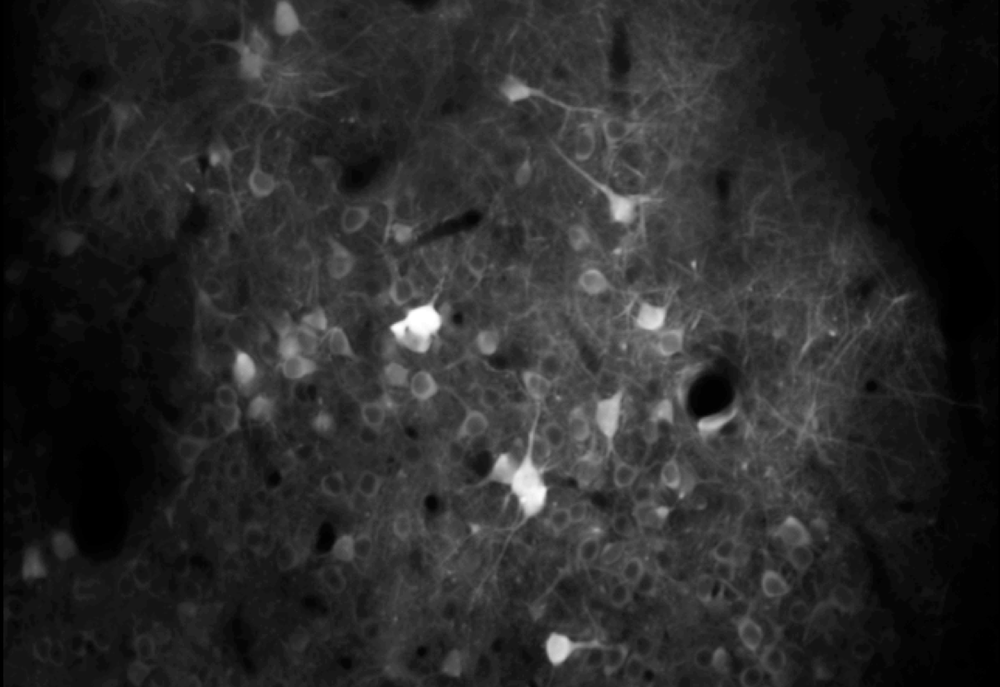
\includegraphics[width=0.5\textwidth]{neurons}
  \caption{A snapshot of neurons labeled with GCaMP6s within a region of the cortex.}
  \label{neurons}
\end{figure}

%%%%%%%%%%%%%%%%%%%%%%%%%%%%%%%%%   DATASET    %%%%%%%%%%%%%%%%%%%%%%%%%%%%%%%%
\section{Dataset}

\subsection{Description}

We have obtained data sets from the Max Planck Institute for Neurobiology 
corresponding to three recording sessions from the same mouse. Each recording 
session consists of multiple time series of fluorescent activity corresponding 
to the neurons within the imaged area. GCaMP6s, a slower decaying member of 
the GCaMP6 family, was used as the calcium sensor in these experiments. The 
first data set consists of activity of neurons in the primary visual cortex 
(V1) that are known to reliably respond to oriented gratings at a certain 
angle (see Figure \ref{fig:tuning}), which are presented to the mouse during 
the trial. An illustration of this setup is shown in Figure \ref{fig:setup}. 
This data will be a useful control for testing our structure learning method 
because we expect that there will be a strong correlation between neural 
activity and the display of specific stimuli. \par

\begin{figure}[ht]
  \centering

  \begin{subfigure}{0.45\textwidth}
    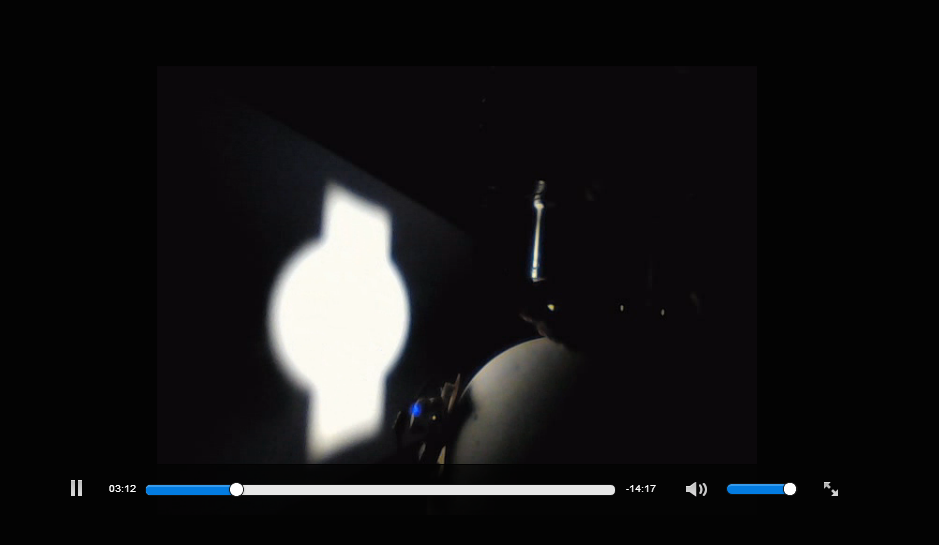
\includegraphics[width=\textwidth]{looming}
    \caption{Stimuli being Presented to the Mouse}
    \label{fig:setup}
  \end{subfigure}
  ~
  \begin{subfigure}{0.45\textwidth}
    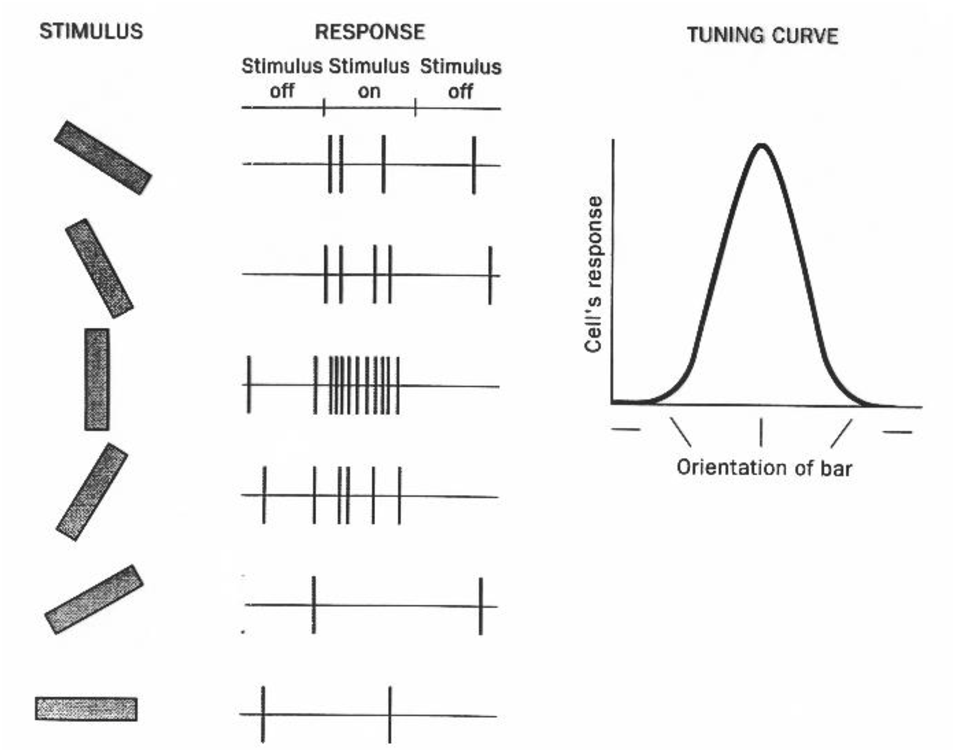
\includegraphics[width=\textwidth]{moving_gratings}
    \caption{Typical Response to Moving Gratings Stimuli}
    \label{fig:tuning}
  \end{subfigure}

  \caption{Showing the Mouse Stimuli and Measuring its Response}
\end{figure}

The remaining data sets track the activity of neurons in the ectorhinal cortex 
during periods of spontaneous activity and the display of novel stimuli. 
Inferring network structure for these time series will allow us to investigate 
the difference between the correlation neurons exhibit during spontaneous 
activity versus when a stimulus is present. \par

\subsection{Pre-Processing}
\label{sec:data}

Each of the neurons in a recording session is represented by a time series of 
noisy fluorescent activity data. Specifically, there are about 24,000 frames 
per neuron, coming from an eight hour recording session. Because the data is 
noisy, it needed to be preprocessed in order to be analyzed effectively.\par

First, we smoothed the data by replacing each point with the average of a 
sliding window (of size 20). The effects of smoothing the data are visualized 
in Figure \ref{fig:smoothing}. Figure \ref{fig:neural_activity} shows just how 
noisy the raw neural activity measurements are. Figure 
\ref{fig:smoothed_neural_activity} shows the effect of our smoothing algorithm
on the data. \par
 
\begin{figure}[ht]
  \centering
  
  \begin{subfigure}{0.45\textwidth}
    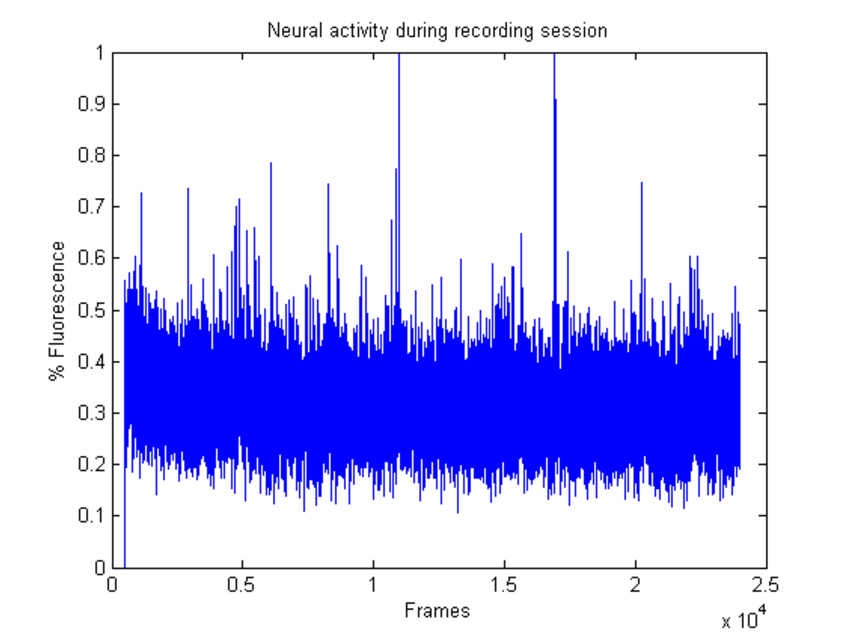
\includegraphics[width=\textwidth]{neural_activity}
    \caption{Raw Neural Activity over Time}
    \label{fig:neural_activity}
  \end{subfigure}
  ~
  \begin{subfigure}{0.45\textwidth}
    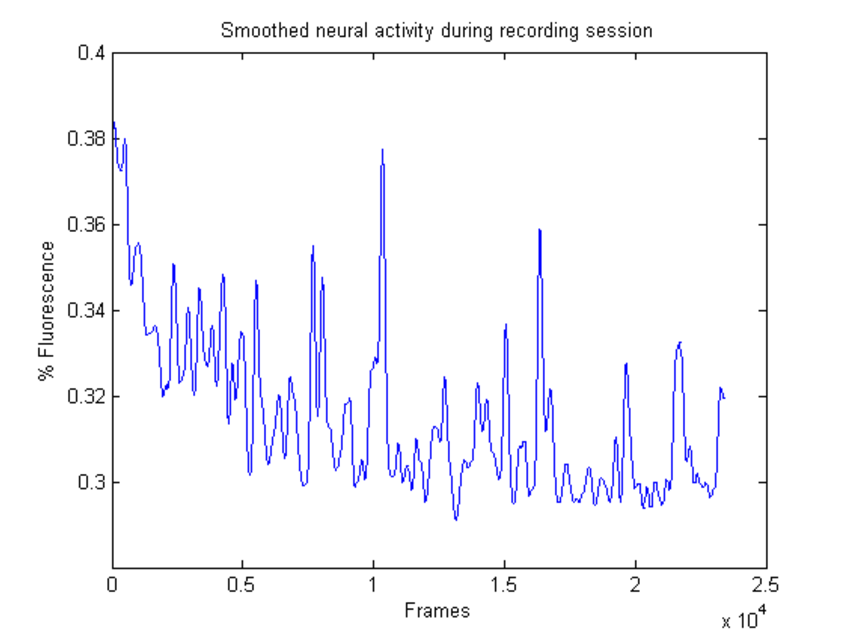
\includegraphics[width=\textwidth]{smooth_neural_activity}
    \caption{Smoothed Neural Activity over Time}
    \label{fig:smoothed_neural_activity}
  \end{subfigure}

  \caption{Smoothing Neural Activity}
  \label{fig:smoothing}
\end{figure}

In order to convert this continuous data into a binary format, we normalized 
it to be in the range $[0, 1]$ and identified spikes based on whether a value 
was larger than a predetermined constant (1.25) times the root mean square of 
a preceding window (of 750 frames). Spikes in the data were indicated as 1s 
whereas the lack thereof were represented by 0s. The spike detection process 
is illustrated in Figure \ref{fig:spikes}.

\begin{figure}[ht]
  \centering

  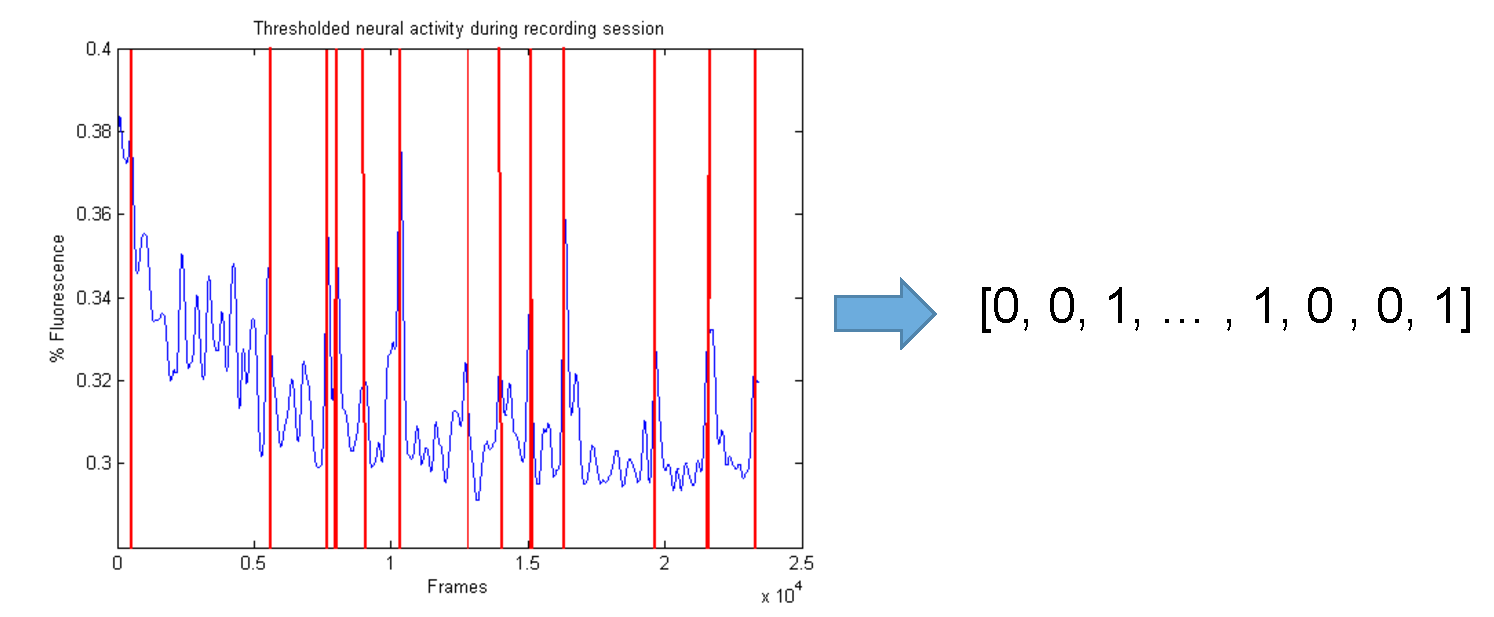
\includegraphics[width=0.9\textwidth]{detecting_spikes}
  \caption{Detecting Spikes in the Neural Activity}
  \label{fig:spikes}
\end{figure}

In order to deal with multiple presentations of the same stimuli throughout 
the recording session (10 of each) as well as sparse stimulus presentations 
(about 25 frames per stimulus presentation), we averaged the values for the 
frames during the presentation of the stimulus and some number of frames 
afterwards (until a new stimulus was shown) across the 10 instances of the 
same stimulus throughout the recording session. \par

%%%%%%%%%%%%%%%%%%%%%%%%%%%%%%%%%    METHOD    %%%%%%%%%%%%%%%%%%%%%%%%%%%%%%%%
\section{Method}

We modelled the local neural circuits as a Bayesian network and infered 
the edges from the correlations of the activity of individual neurons, which 
we treated as binary random variables --– firing or not firing. In order to 
learn the structure, we discretized our continuous series into buckets 
that each represent a single instance of the overall network. \par

We are using the GlobalMIT toolbox for learning the globaly optimal Dynamic 
Bayes Net structure.\cite{globalmit} The toolbox uses the recently introduced 
\emph{mutual information test (MIT)}. It is implemented in both 
Matlab\textsuperscript{\textregistered} and C++. \par

\subsection{The Mutual Information Test}

We will present just a brief overview of this method. For a full discussion of 
this algorithm, we direct an interested reader to.\cite{vinh11} \par

A potential network is scored by the total mutual information shared between 
each node and its parents, less a term that quatifies how statistically 
significant the shared information is. The full discussion shows that the 
first term, considering the total mutual information shared between each node 
and its parents, is equivalent to maximizing the log-likelihood criterion. 
As we know, however, learning a Bayes Net using maximum log-likelihood alone 
risks overfitting the data. In order to avoid this unnecessary complexity, the 
MIT method considers whether the information gained by adding a parent to a 
node is statistically significant. This effectively penalizes a complex 
model. \par

\subsection{Using the Toolkit}

Using the toolkit is rather simple. In order to illustrate the power of the 
toolkit, we give two toy examples that illustrate the output of the toolkit 
given some input. For the output shown in Figure \ref{toy1}, the input is 
a data matrix shown in Table \ref{tab:toy1} where that table has different 
timeslices as columns and different variables as rows. The same format is used
to display the data table shown in Table \ref{tab:toy2} used for the toy 2 
example shown in Figure \ref{toy2}. 

\begin{table}[h]
  \centering
  \begin{tabular}{c |  c | c| c|  c |c| c| c| c| c| c| c| c|c|c|c|c|c|c|c}
    \hline
    1 & 1 & 1 & 1 & 1 & 0 & 0 & 0 & 0 & 0 & 0 & 0 & 0 & 0 & 0 & 0 &0&0&0& 0 \\
    0 & 0 & 0 & 0 & 0 & 1 & 1 & 1 & 1 & 1 & 0 & 0 & 0 & 0 & 0 & 0 &0&0&0& 0 \\
    0 & 0 & 0 & 0 & 0 & 0 & 0 & 0 & 0 & 0 & 1 & 1 & 1 & 1 & 1 & 0 &0&0&0& 0 \\
    0 & 0 & 0& 0 & 0 & 0 & 0 & 0 & 0 & 0 & 0 & 0 & 0 & 0 & 0 & 1 &1&1&1& 1 \\
    \hline
  \end{tabular}
    \caption{Toy1 Dataset}
    \label{tab:toy1}

\end{table}

\begin{table}[h]
  \centering
  \begin{tabular}{c| c| c| c| c| c| c| c|c|c|c|c|c|c|c}
    \hline
    1 & 1 & 1 & 1 & 1 & 1 & 1 & 0 & 0 & 0 & 0 & 0 & 0 & 0 & 0 \\
    0 & 0 & 0 & 0 & 0 & 0 & 1 & 1 & 1 & 1 & 1 & 1 & 1 & 1 & 1 \\ 
    0 & 0 & 0 & 0 & 0 & 0 & 1 & 1 & 1 & 1 & 1 & 1 & 1 & 1 & 1 \\ 
    0 & 0 & 0 & 0 & 0 & 0 & 1 & 1 & 1 & 1 & 1 & 1 & 1 & 1 & 1 \\ 
    \hline
  \end{tabular}
    \caption{Toy2 Dataset}
    \label{tab:toy2}

\end{table}

\begin{figure}[h]
  \centering

  \begin{subfigure}{0.25\textwidth}
    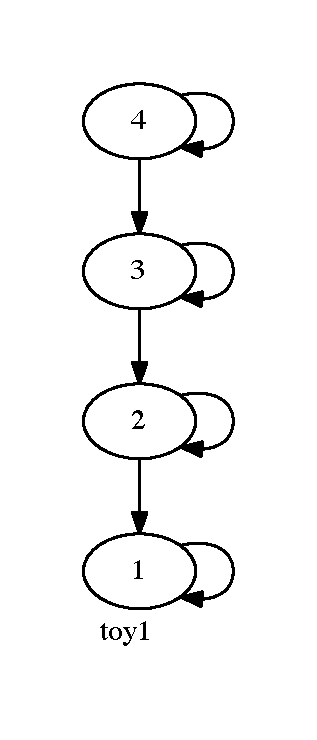
\includegraphics[width=\textwidth]{toy1}
    \subcaption{Toy1 Example Output}
    \label{toy1}
  \end{subfigure}
  ~
  \begin{subfigure}{0.5\textwidth}
    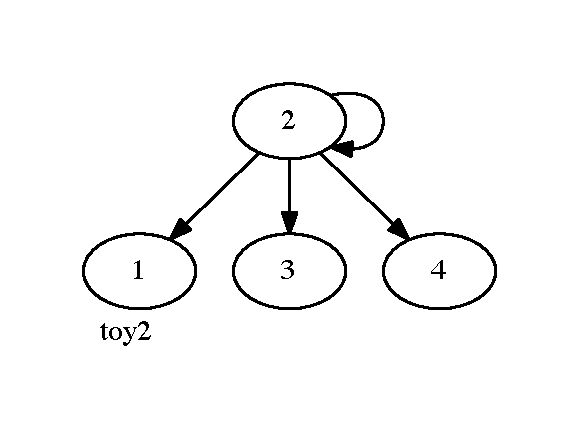
\includegraphics[width=\textwidth]{toy2}
    \subcaption{Toy2 Example Output}
    \label{toy2}
  \end{subfigure}

  \caption{Toy Example Outputs}
  \label{toys}
\end{figure}

\subsection{Implementation Considerations}

The toolkit takes a parameter $\alpha : 0 < \alpha \le 1$ that tunes the rigor 
to which the algorithm will try to fit the model. Lower $\alpha$'s allow for 
a lower degree of uncertainty, so a lower $\alpha$ generates a more accurate 
result but also requires a great deal more computation time. We wanted to use 
as low an $\alpha$ as possible, but due to the data sizes found that the 
lowest we could realistically go was 0.99. This actually turns out to be 
pretty good; the $\alpha$ values used to illustrate how to use the model in 
the toolkit's documentation are 0.95, 0.999, and 0.9999. This leaves us 
feeling satisfied with the $\alpha$ we were able to use.\par

In order to model the entire neural network that we are interested in, we  
needed to make provisions for minimizing the complexity. The 
paper\cite{globalmit} demonstrates a problem in which there are 20 variables 
and 2,000 observations. In the Matlab\textsuperscript{\textregistered} version 
of the toolkit this model takes more than a full day to be learned. Our 
dataset, naively, has as many as 100 variables with 24,000 observations. \par

In order to achieve practical computation times, we had to preform data 
preprocessing as discussed in section \ref{sec:data} of this paper 
including bucketing to get the number of observations down. In addition, the 
paper discusses that the C++ implementation of the toolkit takes only an hour 
to process this same example, leading us to compile and make use of the C++ 
implementation. This was more challenging than using just the tools on the 
Matlab\textsuperscript{\textregistered} side.\par 

Unfortunately, the toolkit made our initial progress very slow. We found that 
with most of permutations of data that we passed to the toolkit, it would 
crash due to memory errors. We compiled the C++ routine and were calling it 
from Matlab\textsuperscript{\textregistered} as per the suggestion in the 
toolkit's documentation, but runs were still taking over an hour and could 
simply die an hour into the computation. In order to solve this problem, we 
used GDB to determine where the crash was coming from.\par

\begin{figure}[h]
  \centering

  \begin{subfigure}{0.48\textwidth}
    {\lstinputlisting[caption=,language=C]{fail.c}}
    \caption{Bug in the toolbox} 
    \label{fig:bug}
  \end{subfigure}
  ~
  \begin{subfigure}{0.48\textwidth}
    {\lstinputlisting[caption=,language=C]{win.c}}
    \caption{Bug fix}
    \label{fig:bugfix}
  \end{subfigure}

\end{figure}

The bug, shown in Figure \ref{fig:bug}, was easy to fix (once found). The 
routine calculates $P^*$. Speaking loosely, this is the max number 
of parents that the algorithm is willing to assign to a node. Then, it 
allocates an array of size $P^*-1$. If $P^* == 0$, there you have your memory 
error. The fix was very simple, as shown in Figure \ref{fig:bugfix}. Since 
$P^* == 0$ implies that the node has no possible parents, we can simply skip 
the computation on that node and avoid the problematic allocation. \par

Although a trivial fix, finding this bug added a lot of time to our work. Once 
we found it, despite having already presented our project to the class, we 
were able to get some really interesting results as you can see in this 
paper.\par

%%%%%%%%%%%%%%%%%%%%%%%%%%%%%%%%%  EVALUATION  %%%%%%%%%%%%%%%%%%%%%%%%%%%%%%%%
\section{Results}
 
We expected that the structure we learned from the first data set will reflect 
the high correlation between neural activity and the presence of particular 
stimuli in V1. After we verified that this was indeed the case, we applied the 
same method to the other data sets in order to learn the network structure of 
the neural circuit in the ectorhinal cortex. \par

\begin{figure}[ht]
  \centering

  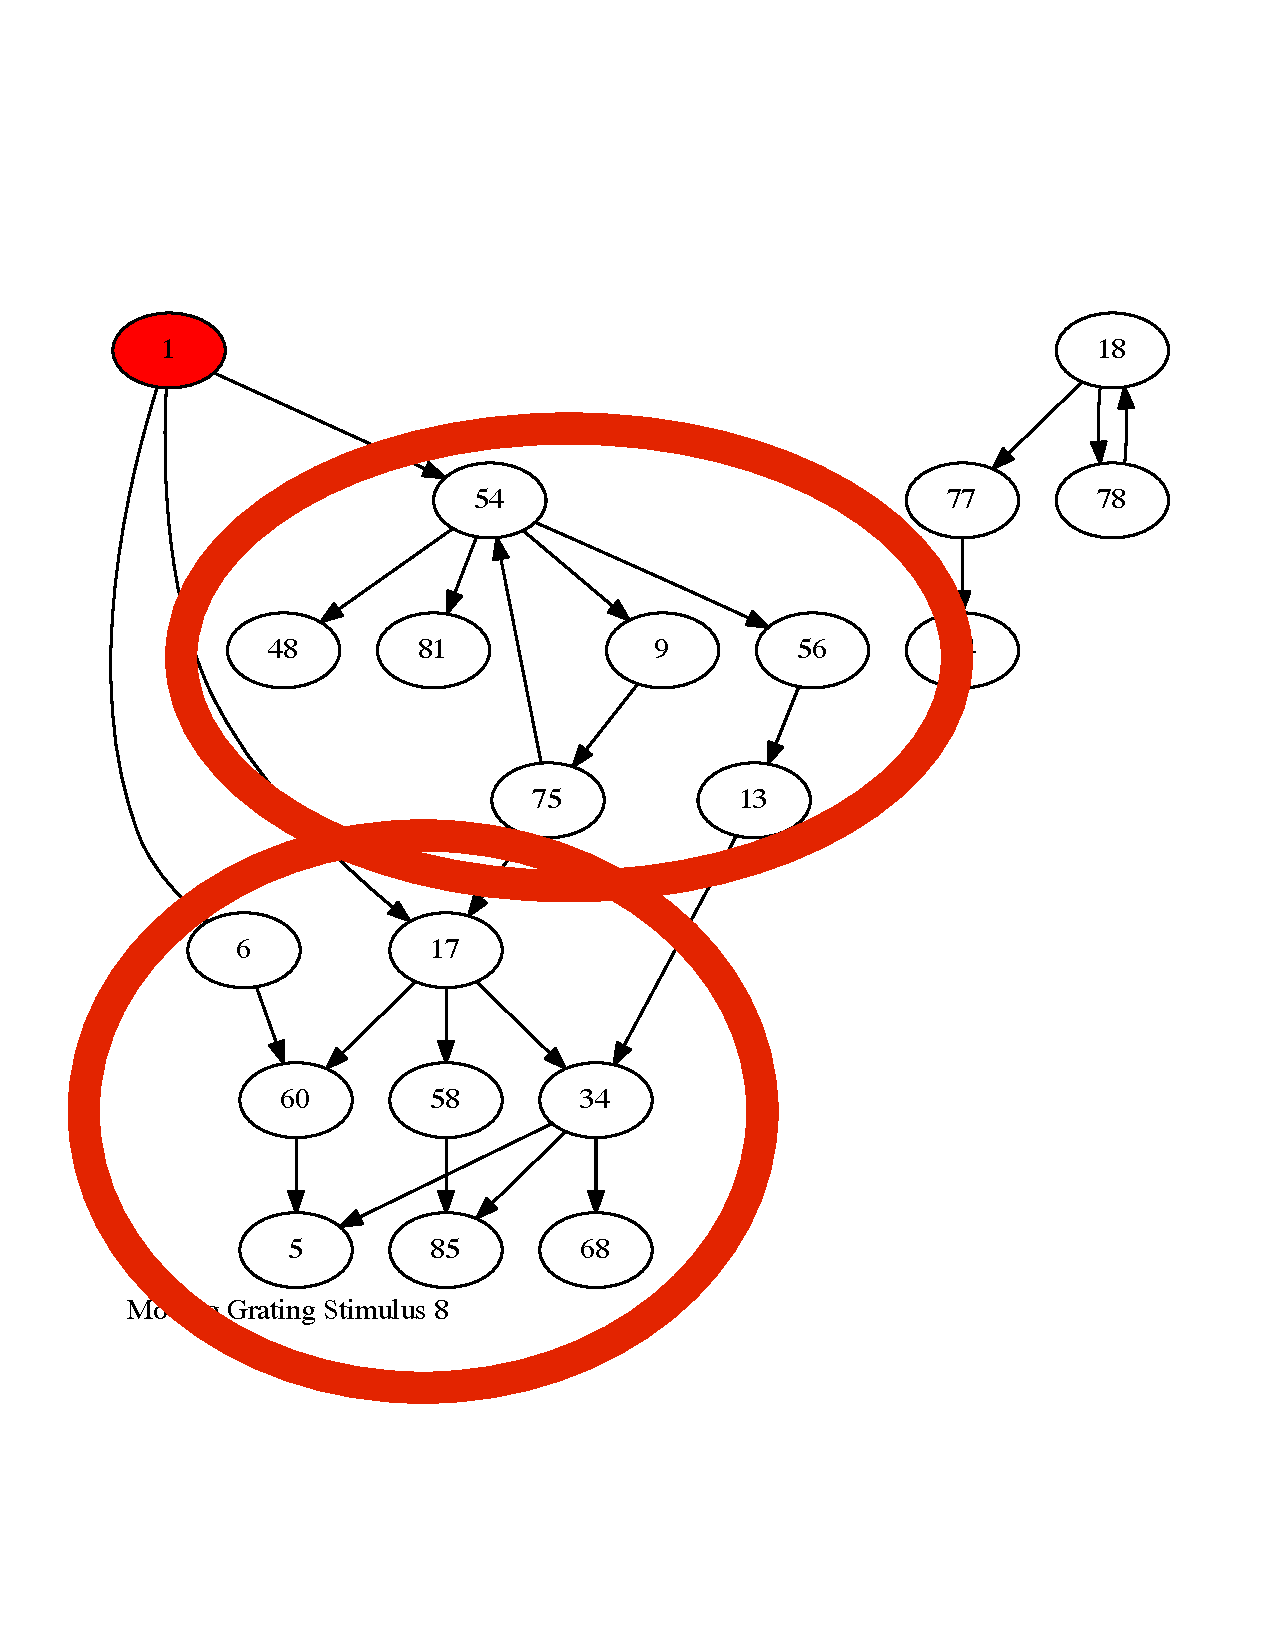
\includegraphics[width=0.5\textwidth]{v1_clusters}
  \caption{Clustering Revealed in the Primary Visual (V1) Cortex}
  \label{fig:v1_clusters}
\end{figure}

Our findings in the primary visual cortex support our expectations. Stimuli 
are found to have a large number of outgoing connections indicating their 
causal relationship to the activation of a set of neurons that are sensitive 
to their presentation. Table \ref{tab:degrees} also shows this in relation to 
the ectorhinal cortex. Additionally, neurons are clustered in separate groups 
as seen Figure \ref{fig:v1_clusters}. This is also indicated by a low network 
average clustering coefficient as shown in Table \ref{tab:v1_clusters}. This 
result makes intuitive sense given neurons that are similarly tuned are likely 
to be active together. \par 

\begin{table}[ht]
  \centering
  \footnotesize

  \begin{tabular}{l|c|c|c|c|c|c|c|c|l}
    \hline
    Moving Grating Stimulus & 1 & 2  & 3  & 4  & 5  & 6  & 7  & 8 \\
    Clustering Coefficient & 0.0079 & 0 & 0.0109 & 0.0099 & 0 & 0 & 0 & 0 \\
    \hline
                        & 9 & 10 & 11 & 12 & 13 & 14 & 15 & 16 & Average\\ 
     & 0.0022 & 0.0139 & 0.0115 & 0.0047 & 0.0118 & 0 & 0.0081 & 0 & 0.0051\\
    \hline
  \end{tabular}

  \caption{Clustering Coefficients for the Primary Visual Cortex with Moving Grating Stimuli}
  \label{tab:v1_clusters}
\end{table}

We also generated tuning curves for each of the neurons based on the 
correlation of their raw activity with the presence of stimuli. One such 
tuning curve is shown in Figure \ref{fig:v1_tuning}. Note that V1 neurons 
classically show two peaks like in the figure because they respond similarly 
to gratings of one angle as those rotated by 180 degrees (like 45 and 225 
degrees for example). From these tuning curves, we also generated measures of 
precision and recall to quantify the reliability of our discovered network 
structures, shown in Table \ref{tab:precision_recall}. Specifically, we test 
that neurons which are found to be tuned to certain stimuli are also children 
of stimuli nodes in our graph. While the results are not spectacular, they are 
also not entirely unexpected, as we lose a significant amount of information 
in converting continuous signals to binary. Overall, these findings validate 
our methodology and suggest that further analyses of less well-understood 
areas of the brain can be made reliably. \par

\begin{figure}[ht] 
  \centering
  
  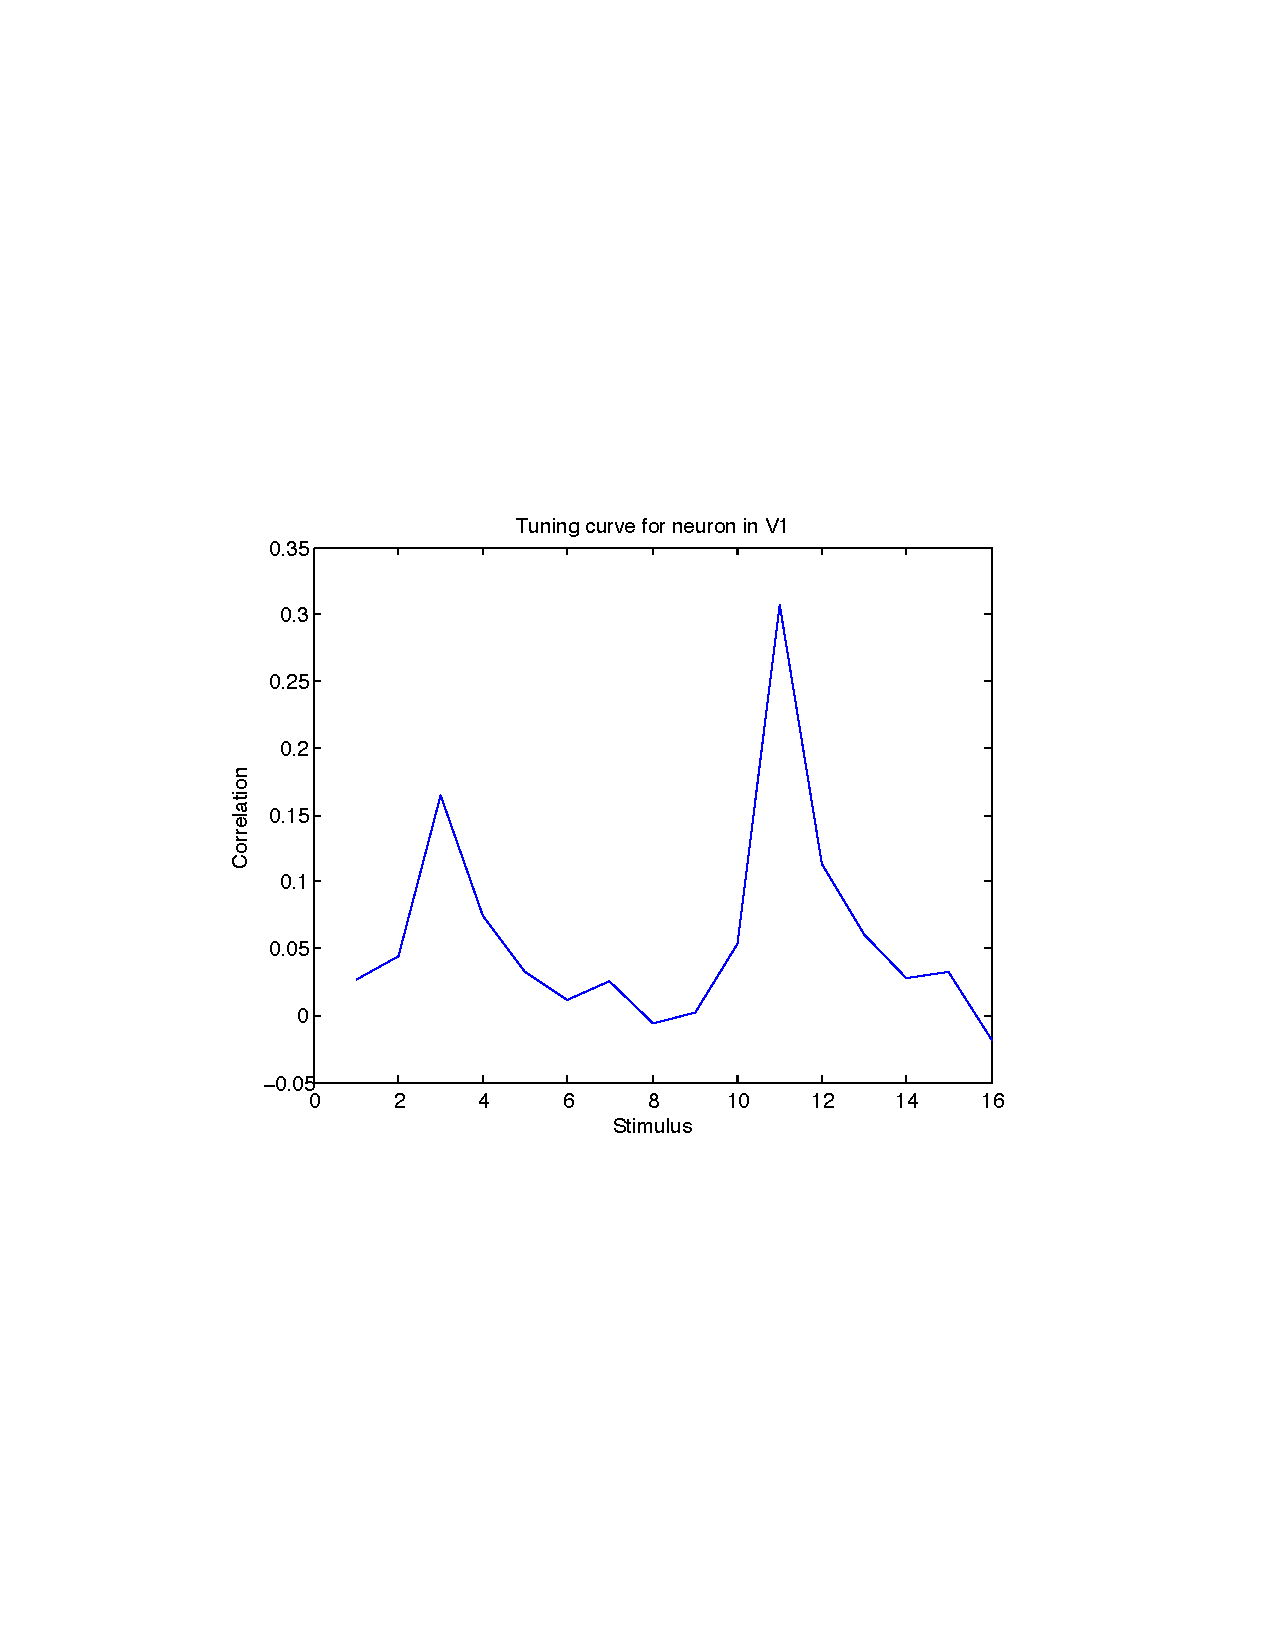
\includegraphics[width=0.5\textwidth]{V1NeuronTuningCurve}
  \caption{Our Measured Tuning Curve for the Moving Gratings}
  \label{fig:v1_tuning}
\end{figure}

\begin{table}[ht]
  \centering
  \footnotesize
  
  \begin{tabular}{l|c|c|c|c|c|c|c|c|c|c|c|c|c|c|c|c}
    \hline
    Stimulus  & 1 & 2 & 3 & 4      & 5      & 6 & 7      & 8      & 9 & 10 & 11     & 12 & 13     & 14 & 15     & 16   \\
    Precision & 0 & 0 & 0 & 0.25   & 0.2    & 0 & 0.25   & 0.3333 & 0 & 0  & 0.3333 & 0  & 0.1429 & 0  & 0.3333 & 0.25 \\
    Recall    & 0 & 0 & 0 & 0.0769 & 0.0769 & 0 & 0.1429 & 0.2    & 0 & 0  & 0.2    & 0  & 0.1111 & 0  & 0.3333 & 0.5  \\
    \hline 
  \end{tabular}

  \caption{Precision and Recall Values for Looming Object Stimuli}
  \label{tab:precision_recall}
\end{table}

Our analysis of the ectorhinal cortex yielded results that were similarly in 
line with our expectations. Specifically, we hypothesized that the ectorhinal 
cortex would respond to the presentation of looming object stimuli because it 
is known to be involved in visual memory and object recognition. Indeed, this 
is what we found: in comparison to the spontaneous activity of the same 
neurons in this area, the network average clustering coefficients (shown in 
Table \ref{tab:ecto_clusters}) for the graphs constructed when looming object 
stimuli were presented were lower, indicating more separation between neurons. 
Qualitatively, this result can be seen in the network structures, as shown in 
Figure \ref{fig:ecto_clusters}. Note that the networks learned from 
spontaneous activity also depict stimuli, as a control for comparison with 
when looming objects were actually presented. That said, treating each 
stimulus as an independent observation of the network structure, the 
difference between the clustering coefficients was not statistically 
significant in a two-tailed t-test ($p$ = 0.3047). \par

\begin{figure}[H]
  \centering

  \begin{subfigure}{0.3\textwidth}
    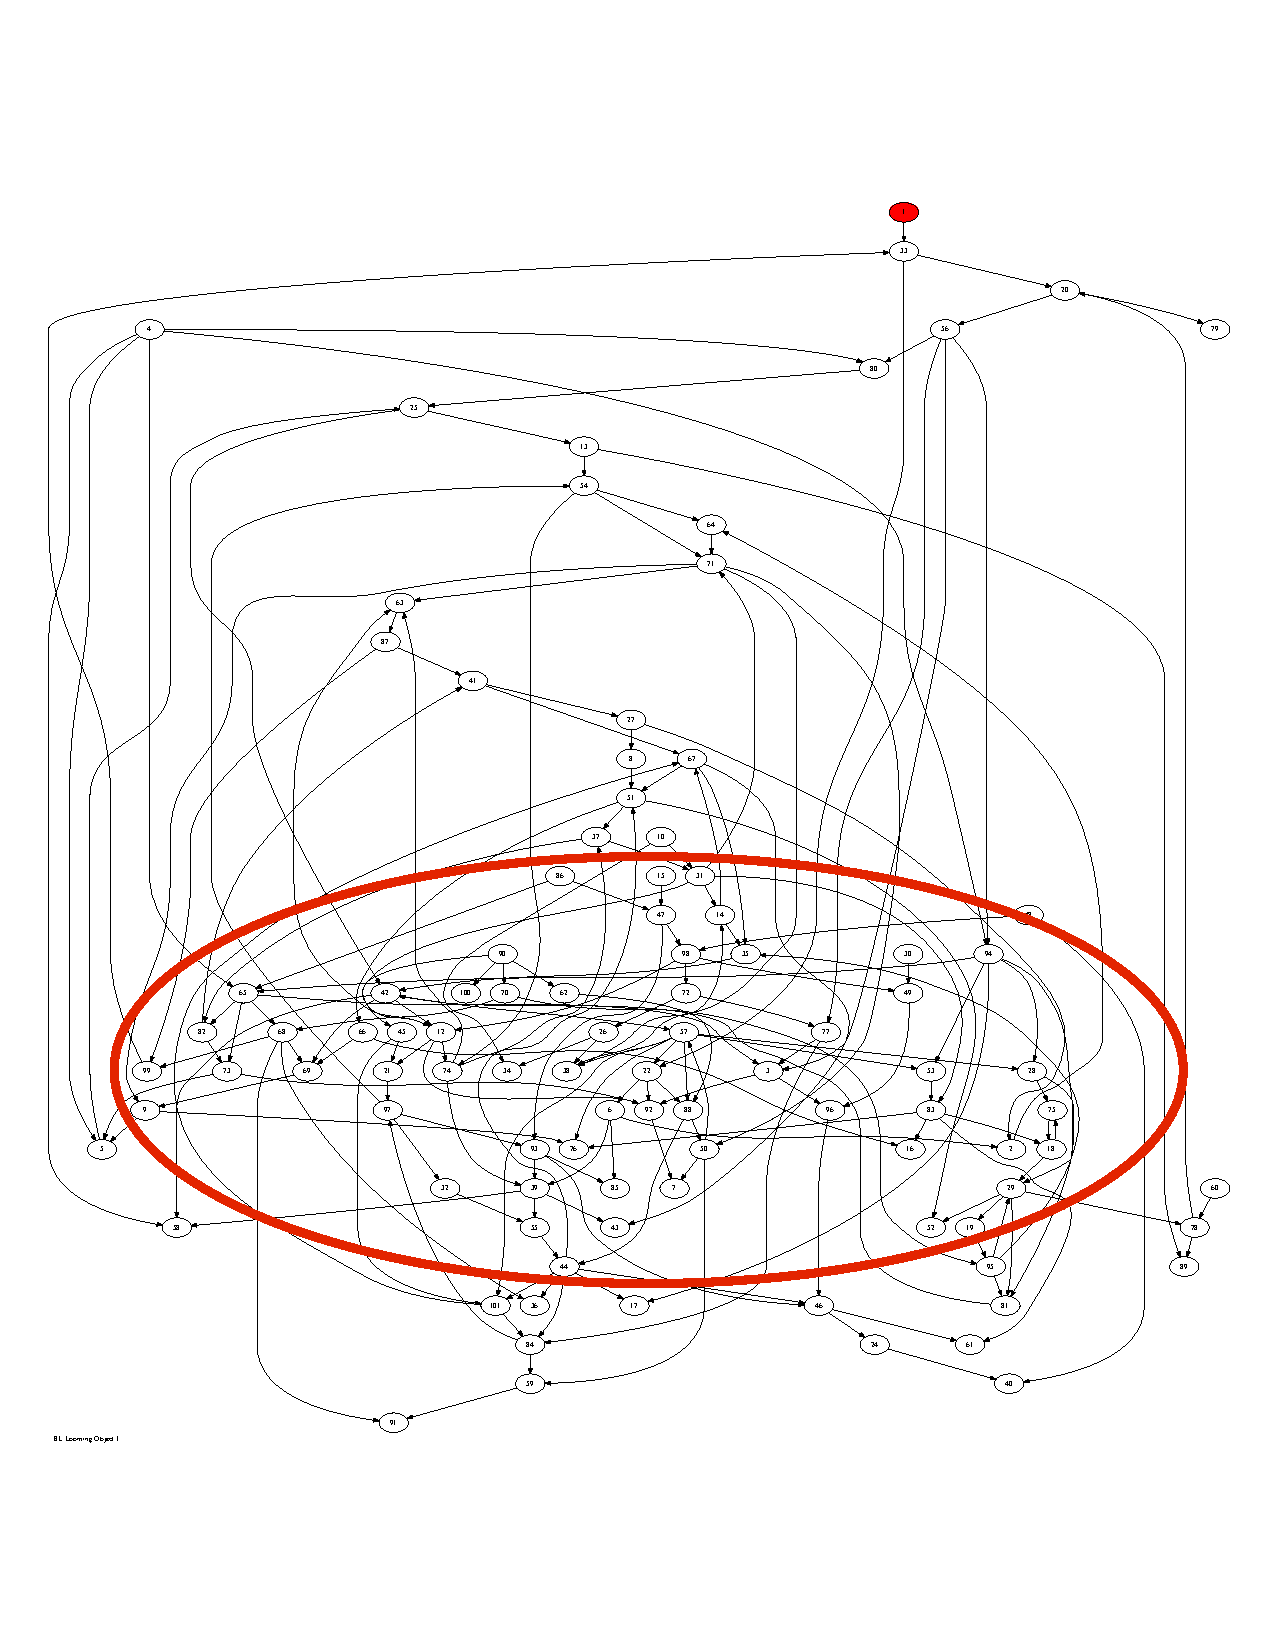
\includegraphics[width=\textwidth]{spont_act_cluster}
    \caption{Spontaneous Activity --- No Clustering}
    \label{fig:spont_clusters}
  \end{subfigure}
  ~
  \begin{subfigure}{0.3\textwidth}
    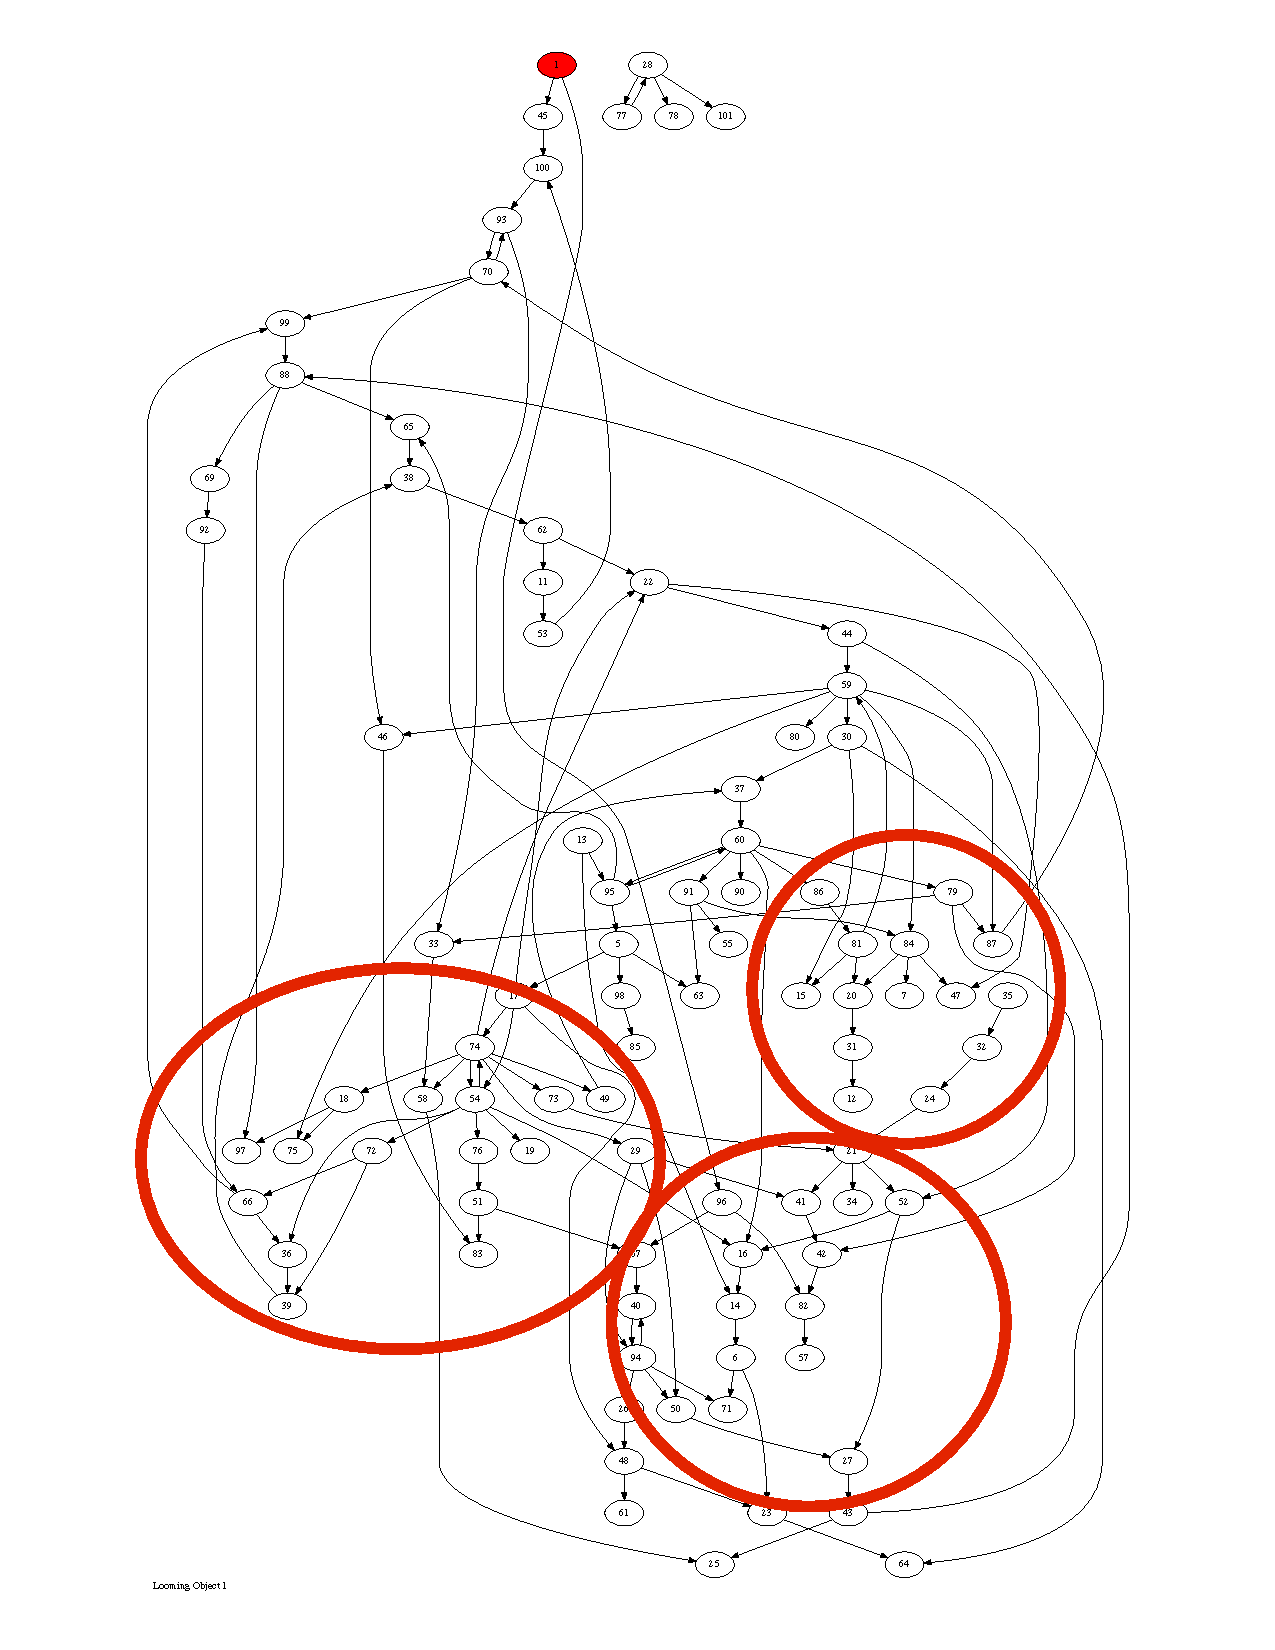
\includegraphics[width=\textwidth]{loom_obj_clusters}
    \caption{Looming Object --- Clear Clustering}
    \label{fig:loom_clusters}
  \end{subfigure}

  \caption{Clustering in the Ectorhinal Cortex}
  \label{fig:ecto_clusters}
\end{figure}

\begin{table}[ht]
  \centering
  \footnotesize

  \begin{tabular}{l|c|c|c|c|c|c|c|c|l}
    \hline
    Stimulus         & 1 & 2 & 3 & 4 & 5 & 6 & 7 & 8 & \\ 
    CC with   & 0.0057 & 0.0203 & 0.0322&0.0205&0.0062&0.0195&0.0233&0 & \\
    CC without&0.0215&0.0174&0.0124&0.0104&0.0027&0.011&0.0097&0.0124 & \\
    \hline
    & 9 & 10 & 11 & 12 & 13 & 14 & 15 & 16 & Average \\
    & 0.01&0.0118&0.0143&0.01&0.0158&0&0.0033&0.0042&0.0123\\
    & 0.0226&0.019&0.0384&0.037&0.0136&0.0332&0.0323&0.0163&0.0194\\
    \hline
  \end{tabular}

  \caption{Clustering Coefficients (CC) for the Ectorhinal Cortex with and without Looming Object Stimuli}
  \label{tab:ecto_clusters}
\end{table}

An analysis of the tuning curves from neurons in these two conditions reveals 
that the presence of stimuli also leads to more organized activity, shown in 
Figure \ref{fig:ecto_tuning_curves}. In support of this claim, the average 
outdegree of stimuli in the networks produced from spontaneous activity was 
only 3.1875, compared to 3.8125 for graphs learned from recordings during 
which looming objects were presented, as shown in Table \ref{tab:degrees}.\par

\begin{figure}[ht]
  \centering
  
  \begin{subfigure}{0.45\textwidth}
    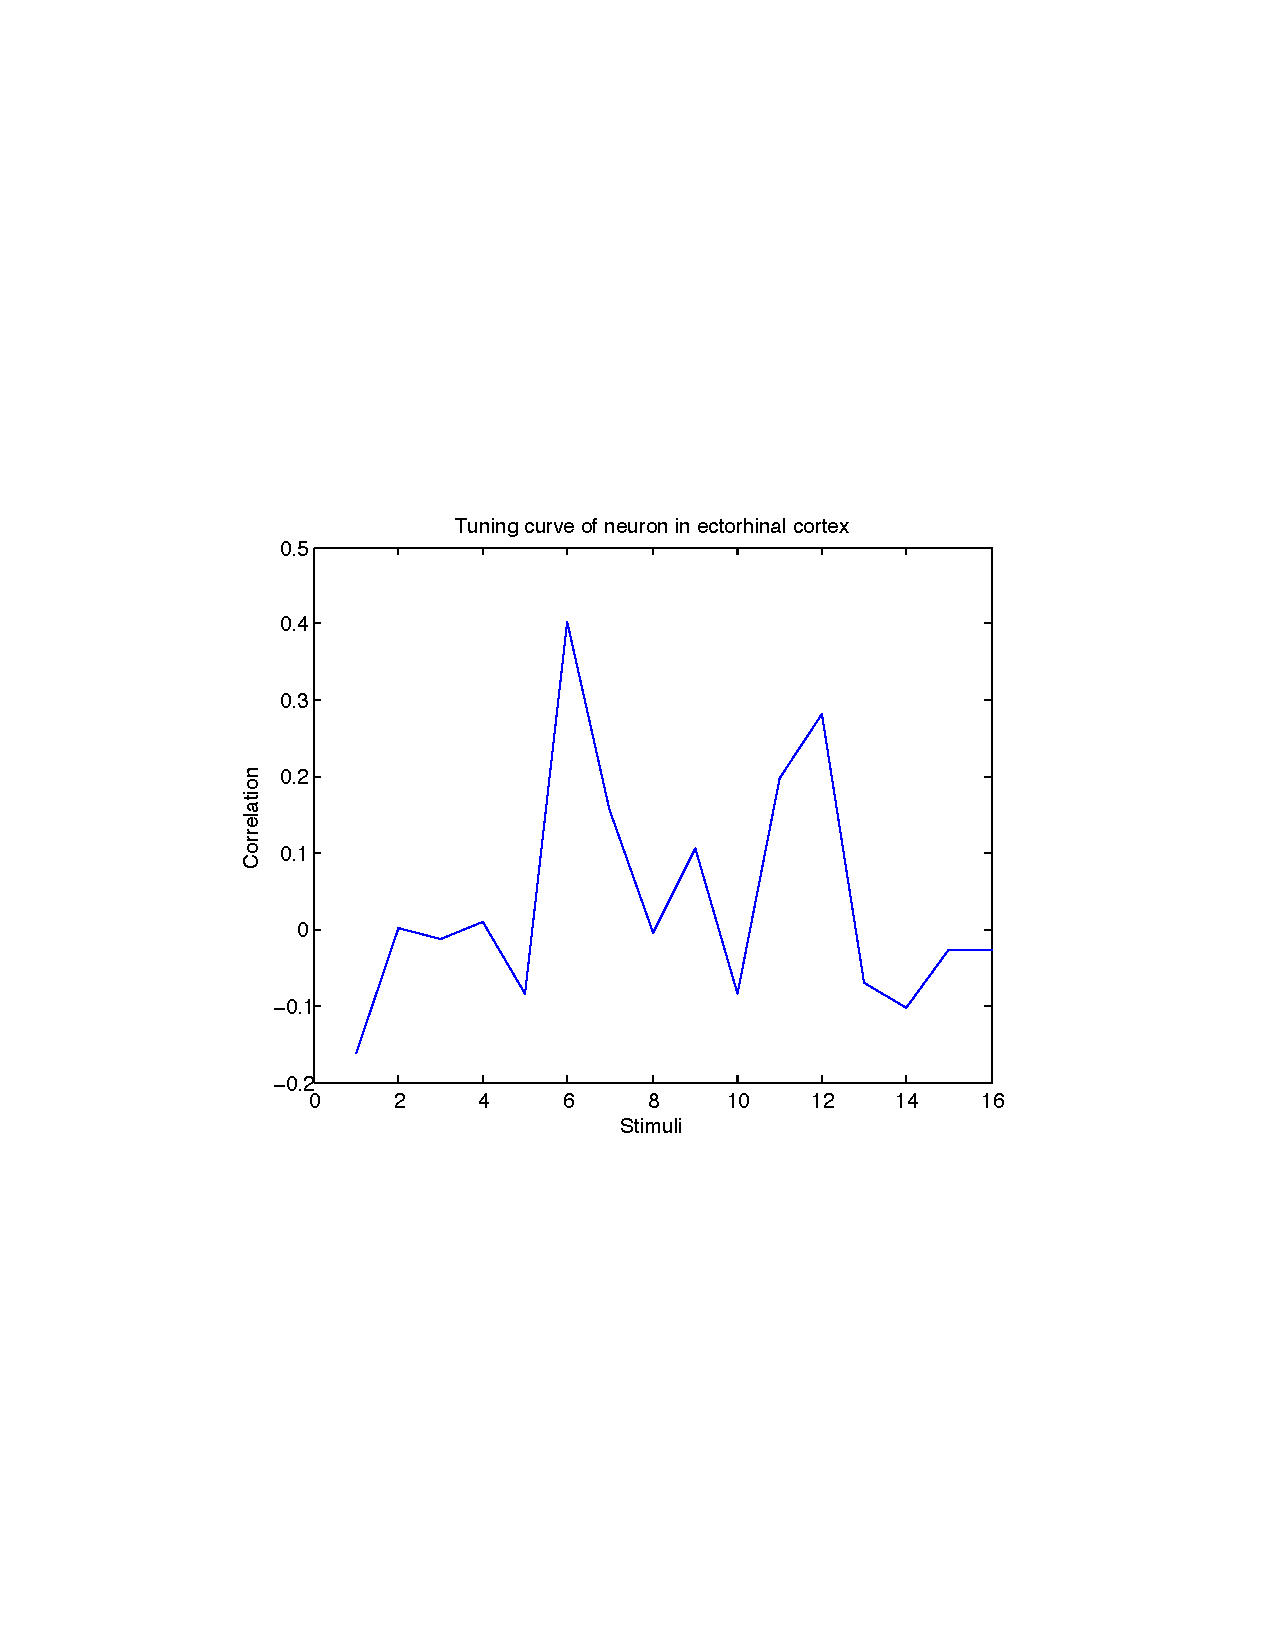
\includegraphics[width=\textwidth]{ECNeuronTuningCurve_LoomObj}
    \caption{With Stimuli}
    \label{fig:loom_obj_tuning}
  \end{subfigure}
  ~
  \begin{subfigure}{0.45\textwidth}
    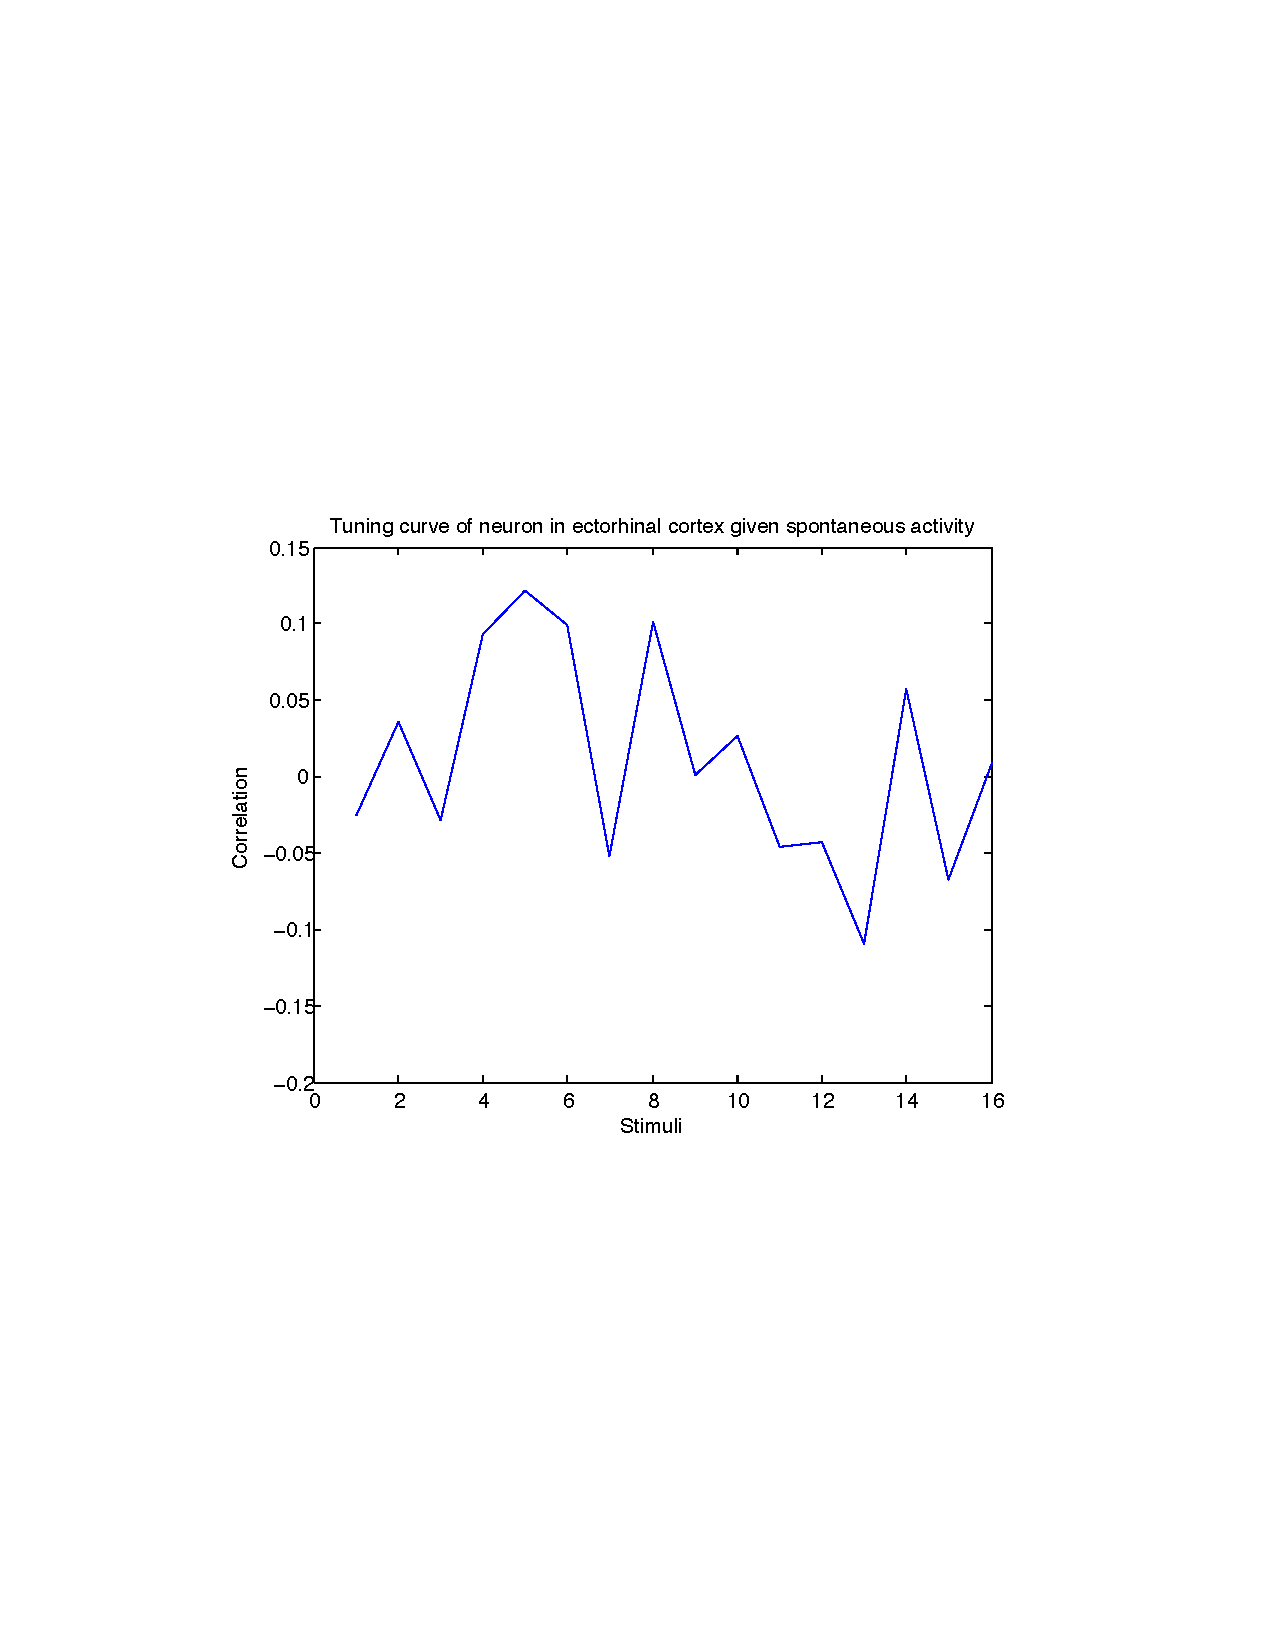
\includegraphics[width=\textwidth]{ECNeuronTuningCurve_Spont}
    \caption{Spontaneous Activity}
    \label{fig:spont_tuning}
  \end{subfigure}

  \caption{Tuning Curves from the Ectorhinal Cortex}
  \label{fig:ecto_tuning_curves}
\end{figure}

\begin{table}
  \centering

  \begin{tabular}{l|l}
    \hline
    Region           & Average Out Degree \\
    \hline
    Primary Visual   & 4.125              \\
    \hline 
    EC - Stimulus    & 3.8125             \\
    \hline
    EC - No Stimulus & 3.1875             \\ 
    \hline
  \end{tabular}

  \caption{Average Out Degree of Source Node in the Primary Visual and Ectorhinal (EC) Cortexes}
  \label{tab:degrees}
\end{table}

Overall, these results support our prediction that neurons in the ectorhinal 
cortex would exhibit more organized activity when the mouse is presented with 
looming object stimuli. For this reason, we do consider our project to be a 
successful look into the neural clustering in the ectorhinal cortex.\par


%%%%%%%%%%%%%%%%%%%%%%%%%%%%%%%%%  FUTURE WORK %%%%%%%%%%%%%%%%%%%%%%%%%%%%%%%%
\section{Future Work}

With more time, we would suggest a few different ways to take this work even 
further.\par

First, we could tune the hyperparameter $\alpha$. This parameter encodes the 
degree to which the algorithm is going to penalize complexity. We chose a 
parameter based primarily on runtime. It is possible that a more closely tuned 
$\alpha$ could lead to better results. \par

Additionally, we would have liked to get our hands on a dataset from a third 
recording session in the ectorhinal cortex. The two that we processed were 
spontaneous activity and during the presentation of novel stimuli. We think 
that it would be interesting to examine the response of the same neurons 
during the presentation of learned stimuli. As explained in our introduction, 
we could hypothesize that the neurons would become tuned as stimuli are 
learned. We think that our work could be the starting point for exploring that 
hypothesis. \par

In order to make our problem tractable, we made some simplifying assumptions. 
For example, we treated the neurons as firing or not firing. In reality, the 
connections between neurons is not binary. In the future, we think that trying 
to infer edge weights in addition to network structure could provide even more 
valuable insight into the connectivity of these neural networks. \par

Finally, we propose work completely different from what we've done. We think 
that it could be interesting to use a hidden markov model to attempt to 
infer the presence of a specific stimulus given only the neural response 
data from the mouse. Although applications seem far-fetched now, we can 
imagine a world in which using just the activity in the brain to reproduce 
what the eyes are seeing could be very useful. Even know, it would be very 
cool. \par

\section{Conclusion}

Overall, we are pleased with the work that we did on this project. We were 
able to use the power of probabalistic graphical models to draw very 
interesting conclusions about the structure of local neural circuits in mouse 
ectorhinal cortex. We consider this project a success; we found interesting 
results while solidifying our understanding of topics that we studied in the 
course. Although there is a lot of room for future work, we think that our 
progress in this area was somewhat novel and a good start towards 
understanding neural circuits in mouse ectorhinal cortex. \par

\bibliographystyle{plain}
\bibliography{bibliography}

\newpage
\appendix
\section{Visualizing our Results}

Here, we are including graphical representations of our results. All of these 
graphs have been processed after they were output by the GlobalMIT algorithm. 
We removed incoming edges from the source node. Unfortunately, we had no way 
to incorporate the a priori knowledge that no neuron can have a causal 
influence on the stimulus, so we had to modify our model after the fact to 
encode this knowledge. We also colored the source node red for the sake of 
clarity. \par

Graphs labeled ``Moving Grating Stimulus'' correspond to measurements in the 
primary visual cortex (V1) in response to gratings at specific orientations 
being presented to the mouse. These were our baseline --- we knew what we 
expected to see from this data, so we used it to validate the performance of 
our methodology. Stimuli 1 through 16 correspond to gratings at different 
angles. \par

Graphs labeled ``BL Looming Object'' correspond to measurements in the 
ectorhinal cortex without the prescence of a stimulus, random activity. These 
allowed for us to measure the effect of a looming object stimulus on the 
neural activity in the region compared to random activity. \par

Graphs labeled ``Looming Object'' correspond to measurements in the ectorhinal 
cortex during the presentation of novel stimuli. This was the dataset that we 
were most interested in exploring. Stimuli 1 through 16 correspond to stimuli  
of different shapes. \par

%%%%%%%%%%%%%%%%%%%%%%%%%%%%%%%%%%% MOVING GRATING STIMULI %%%%%%%%%%%%%%%%%%%%

\newpage
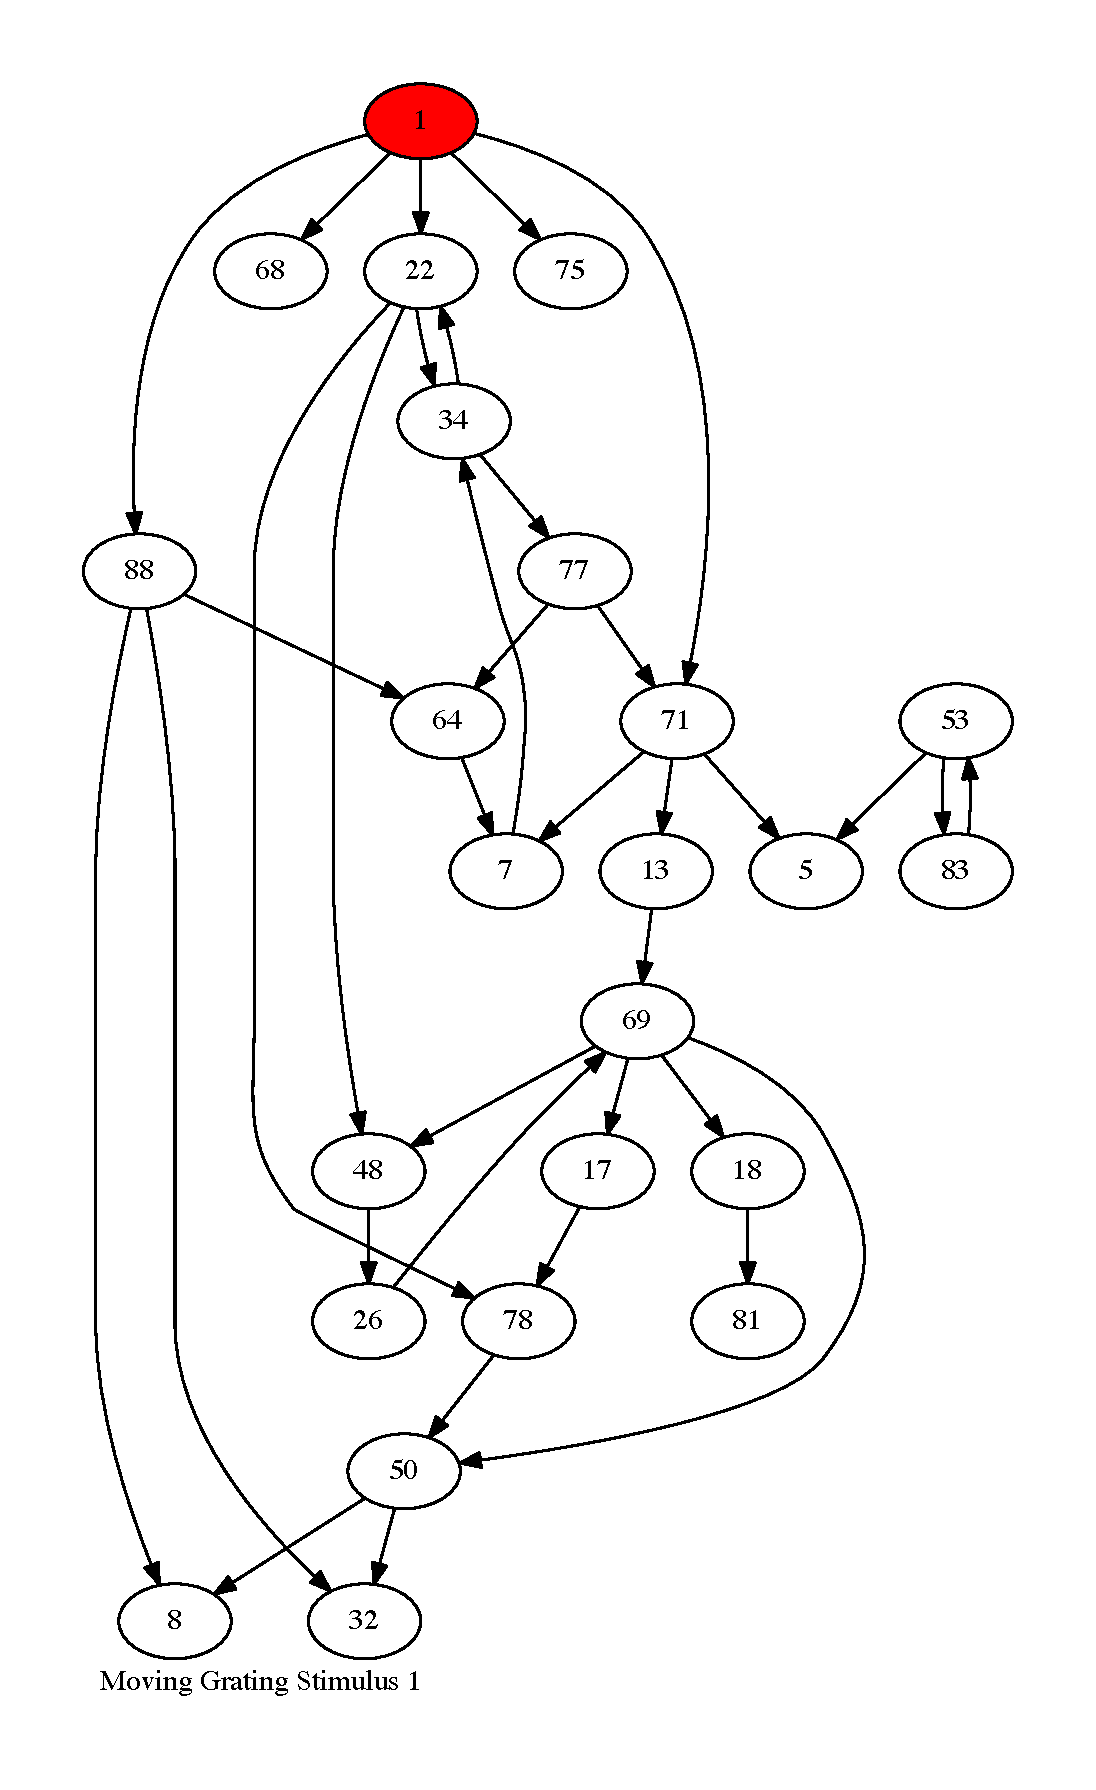
\includegraphics[max height=\textheight,max width=\textwidth]{stim_mov_grat/stim1_pp.pdf}

\newpage
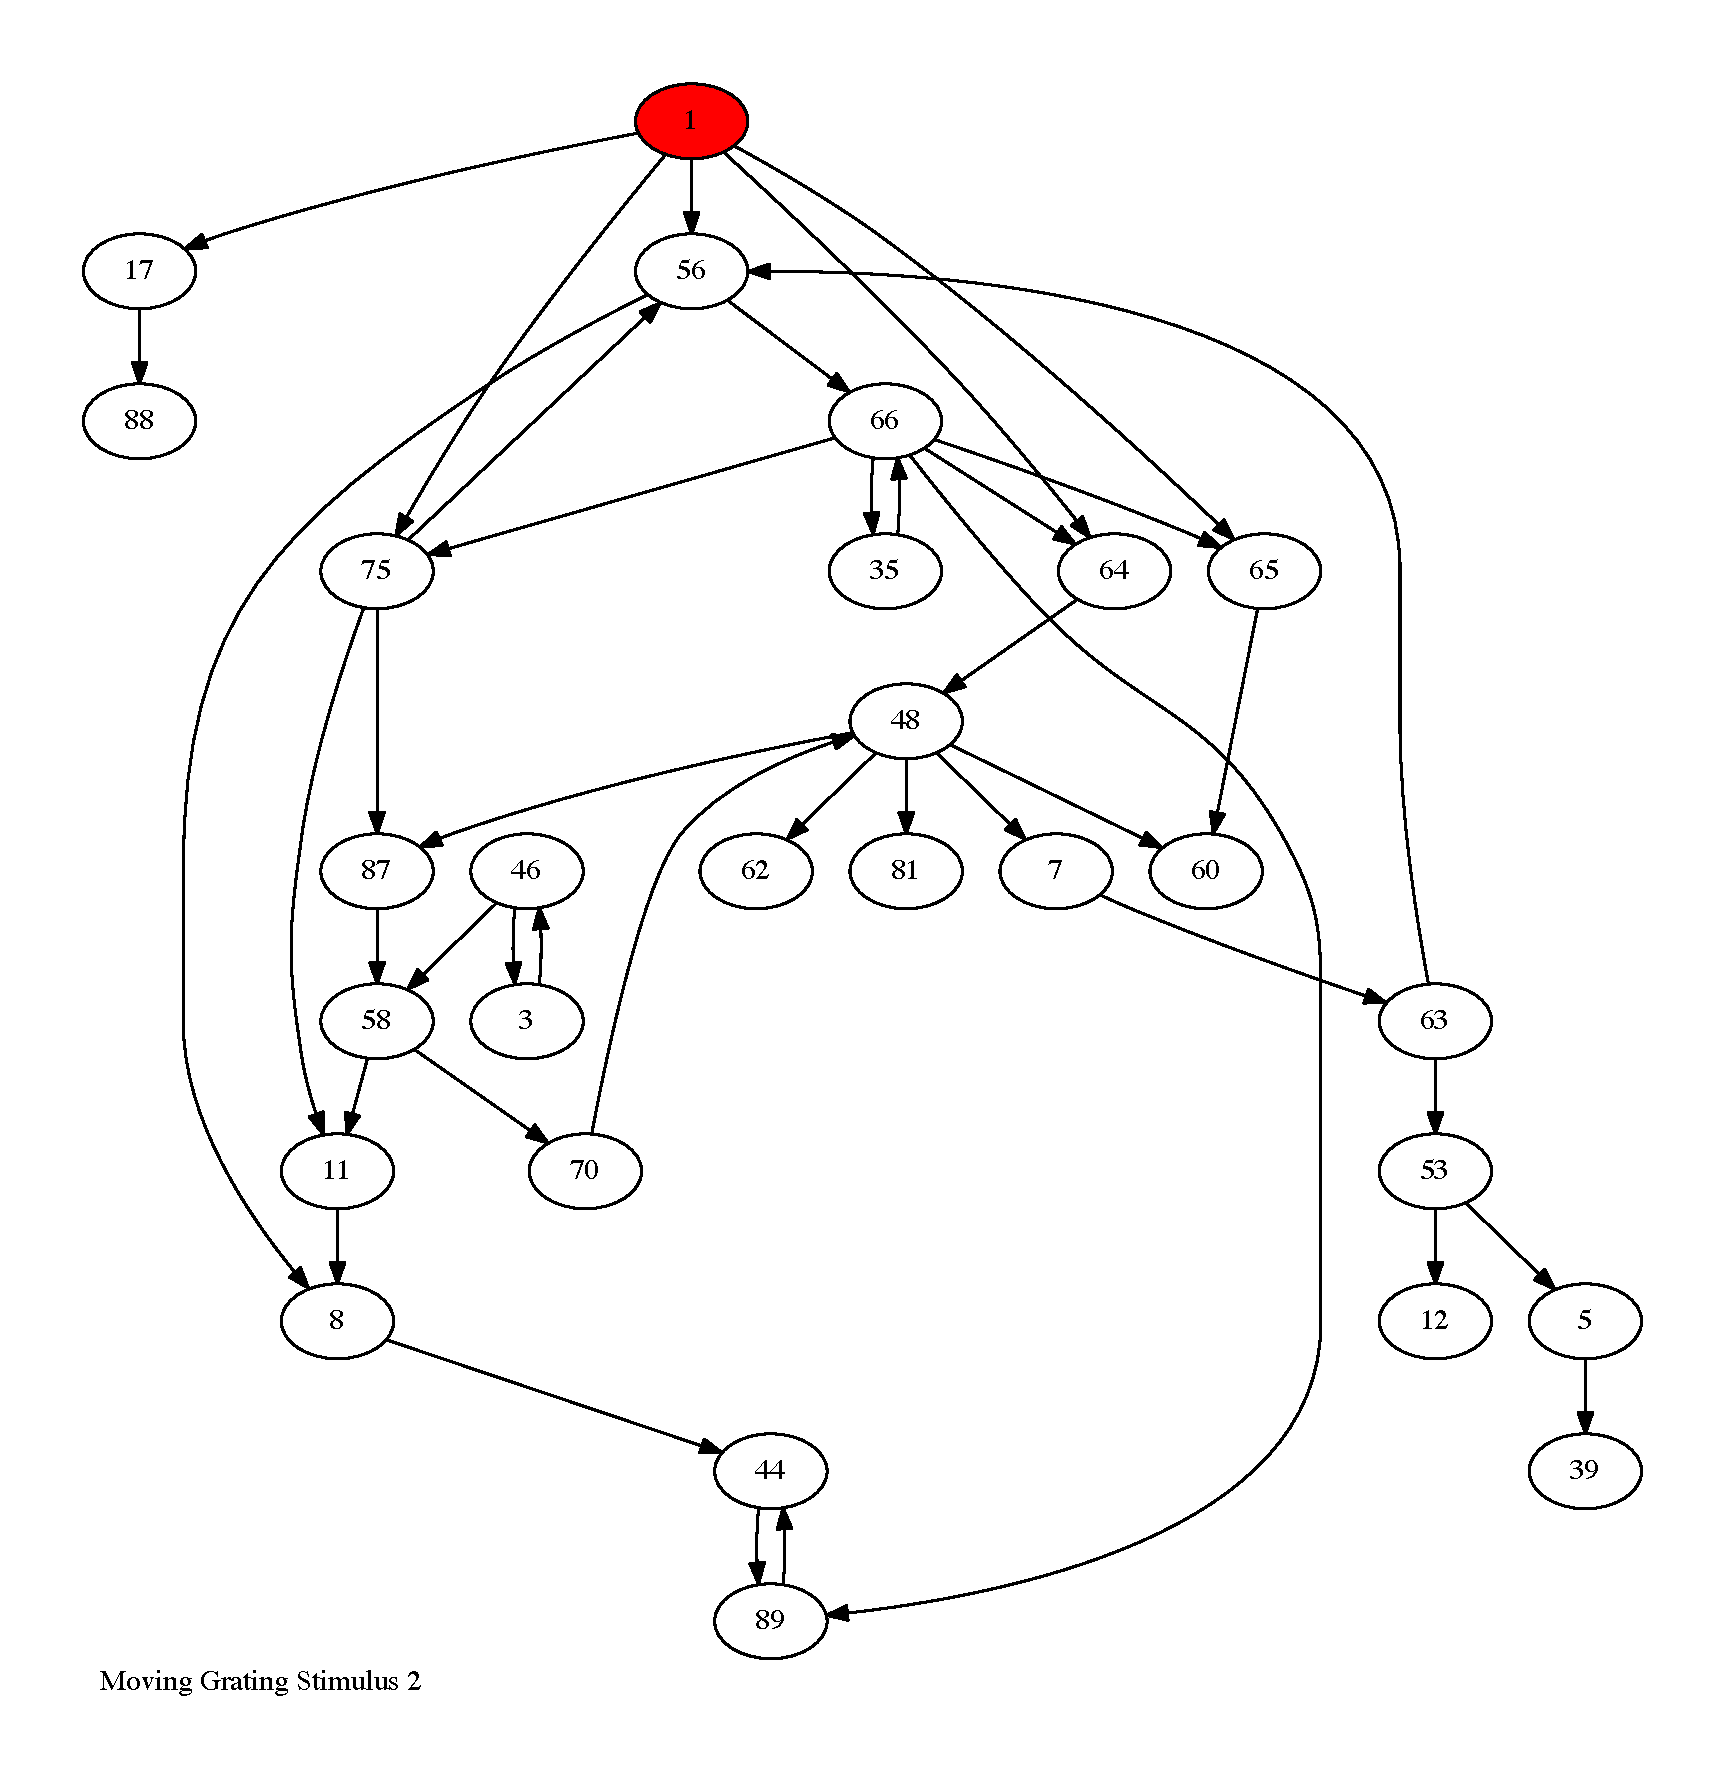
\includegraphics[max height=\textheight,max width=\textwidth]{stim_mov_grat/stim2_pp.pdf}

\newpage
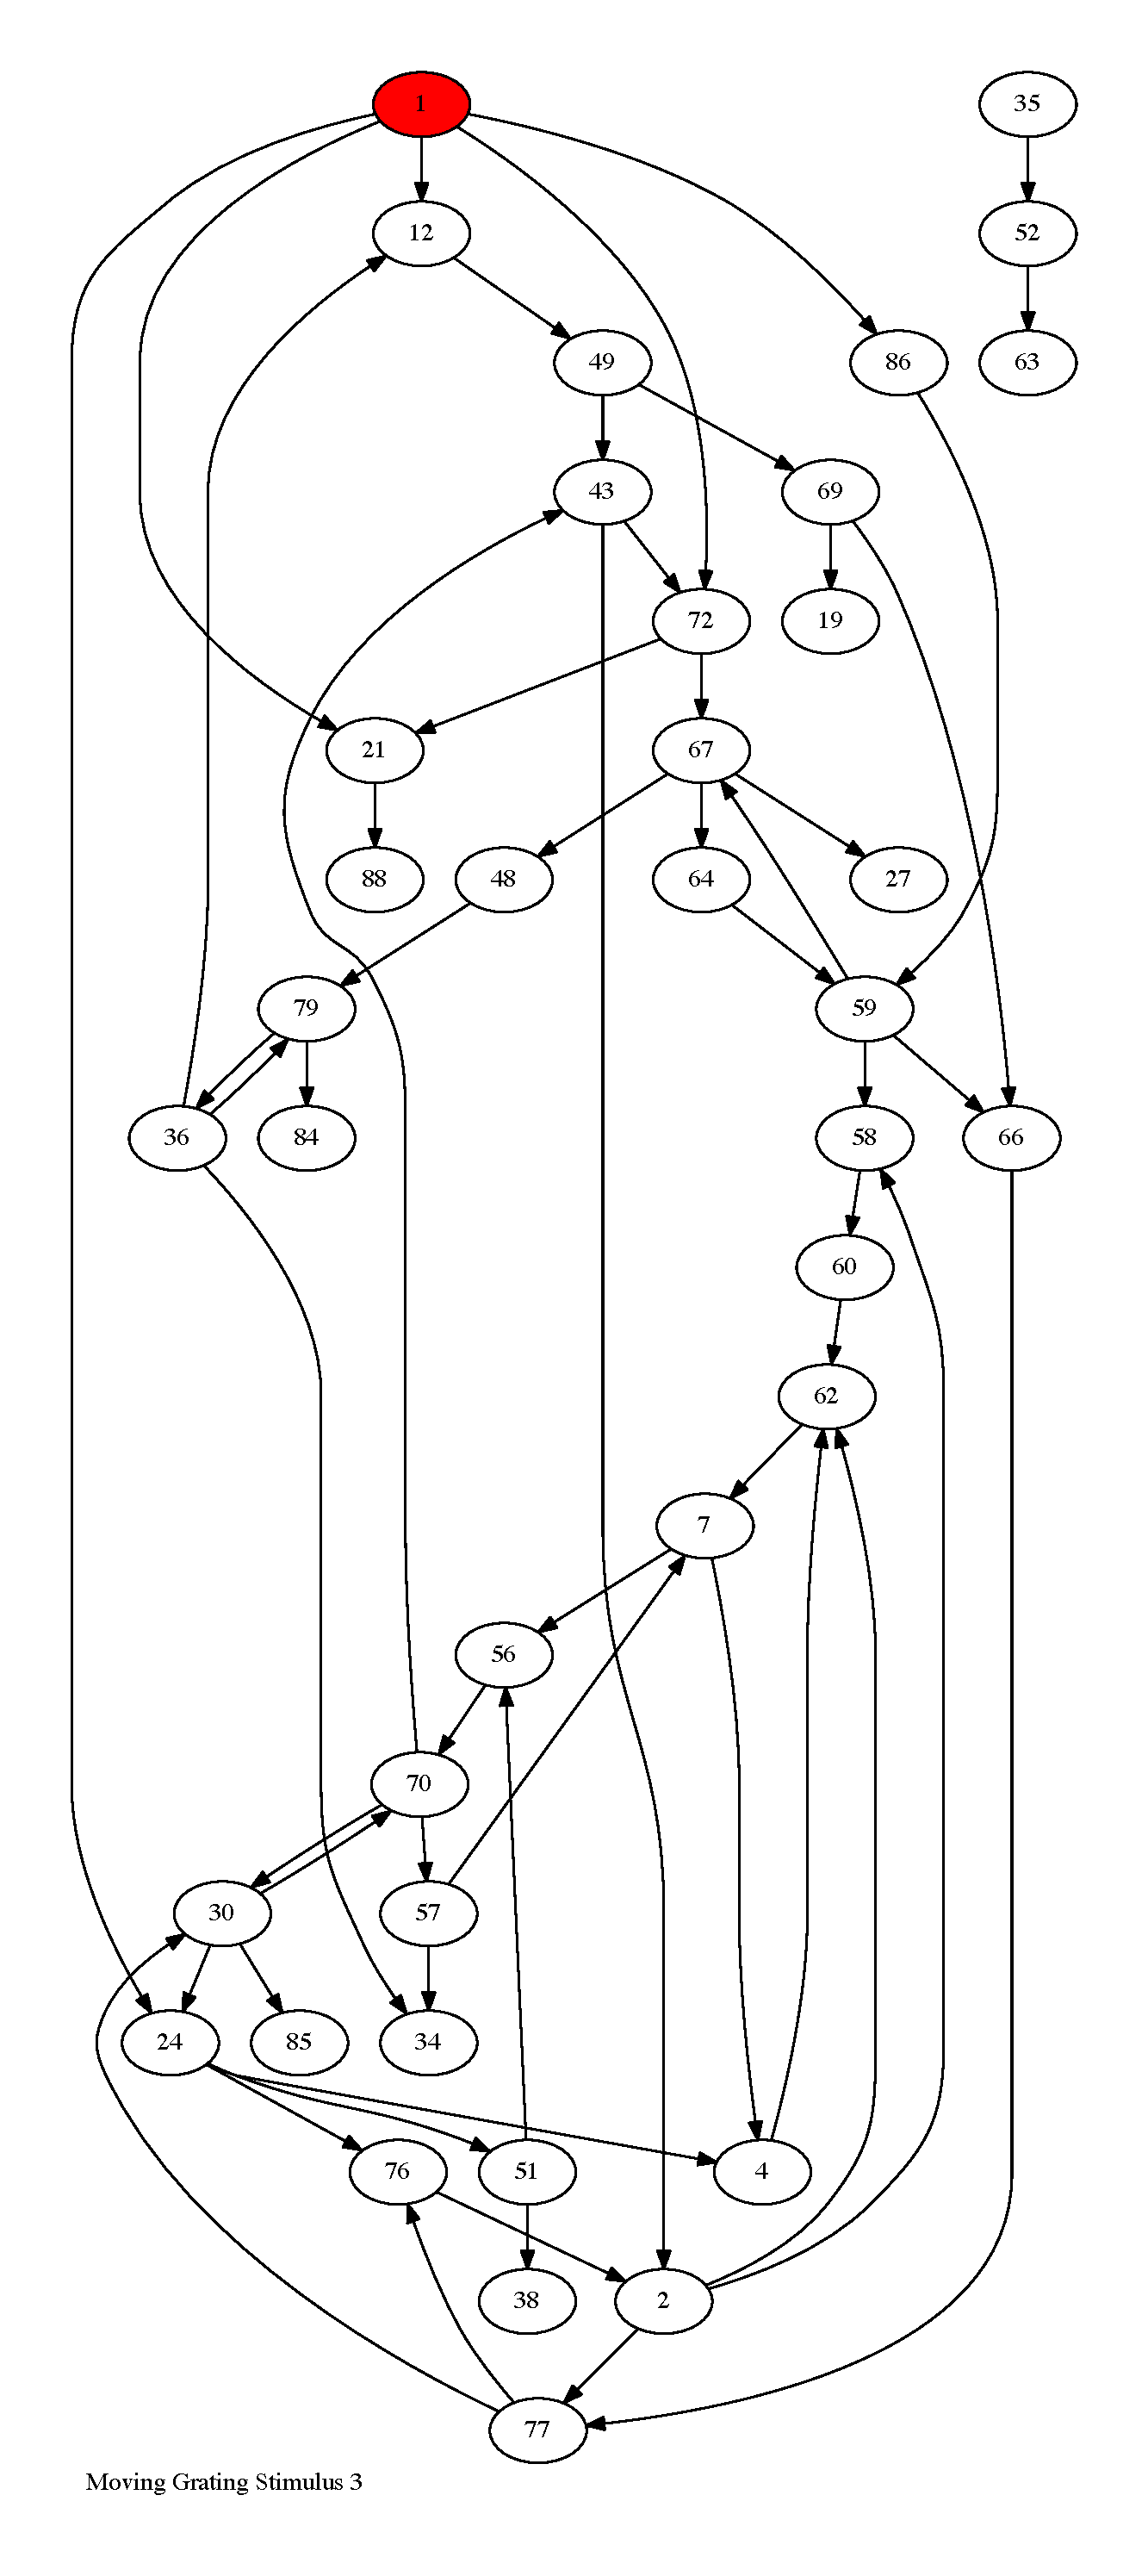
\includegraphics[max height=\textheight,max width=\textwidth]{stim_mov_grat/stim3_pp.pdf}

\newpage
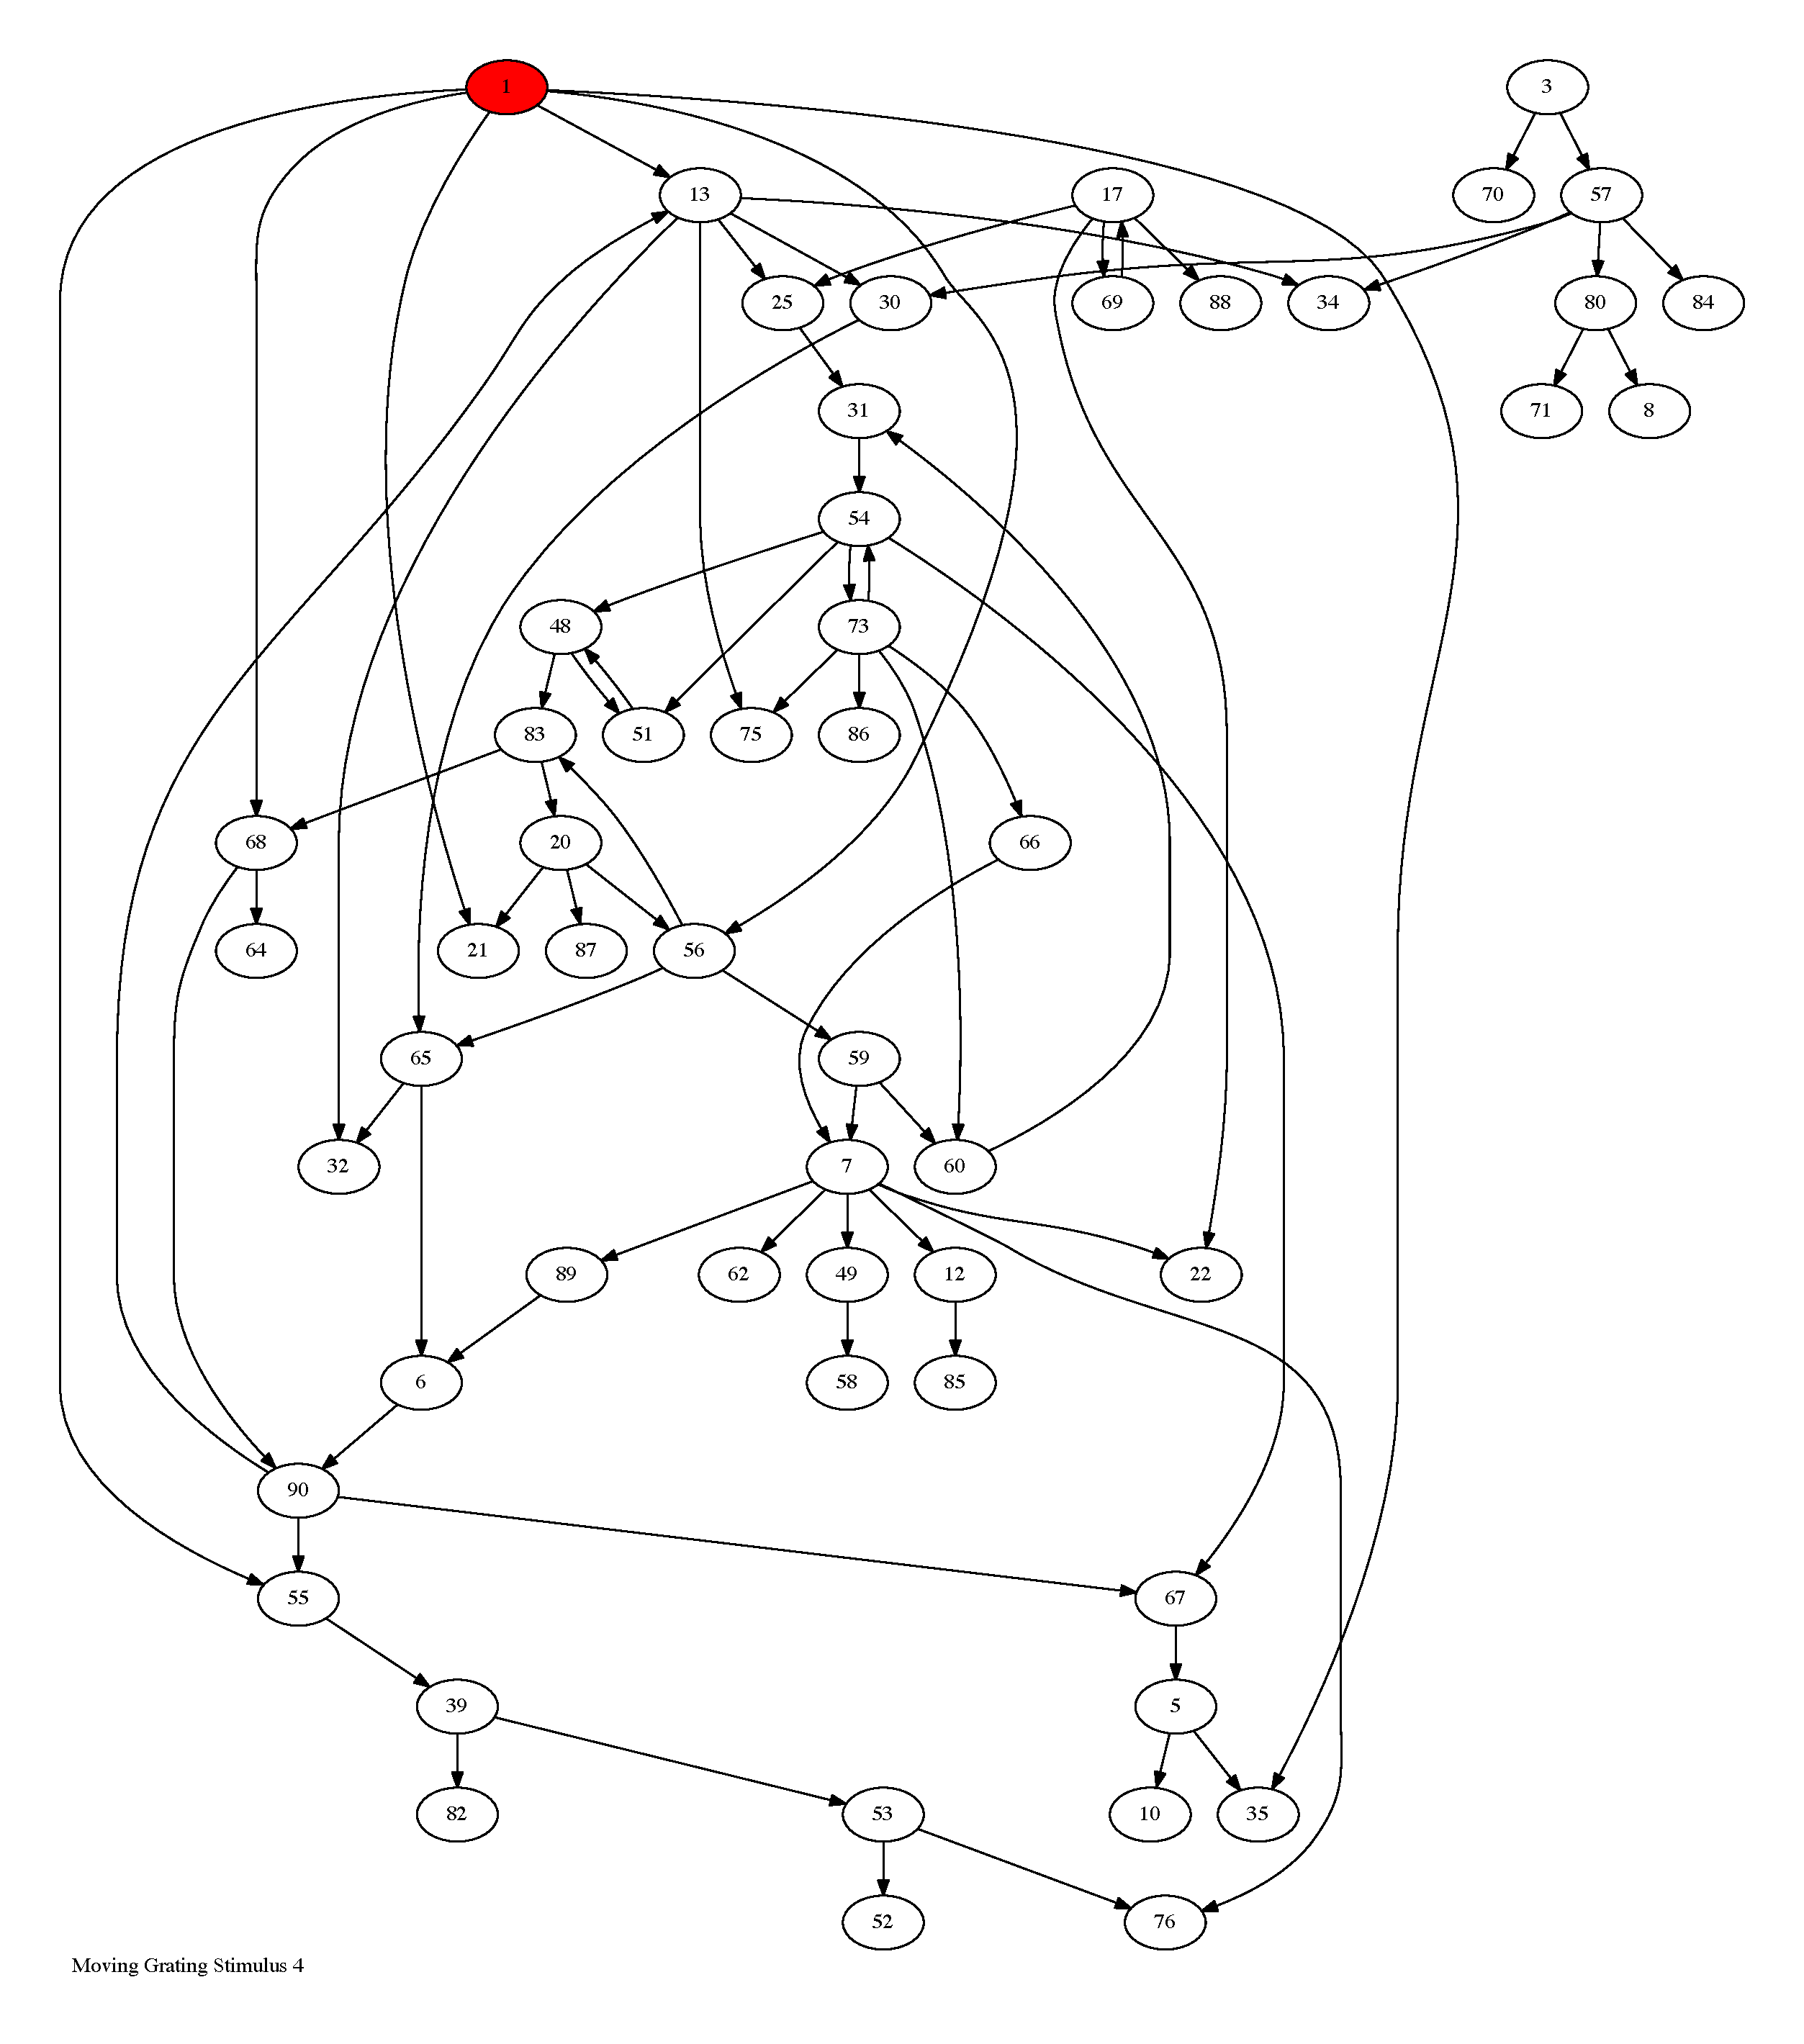
\includegraphics[max height=\textheight,max width=\textwidth]{stim_mov_grat/stim4_pp.pdf}

\newpage
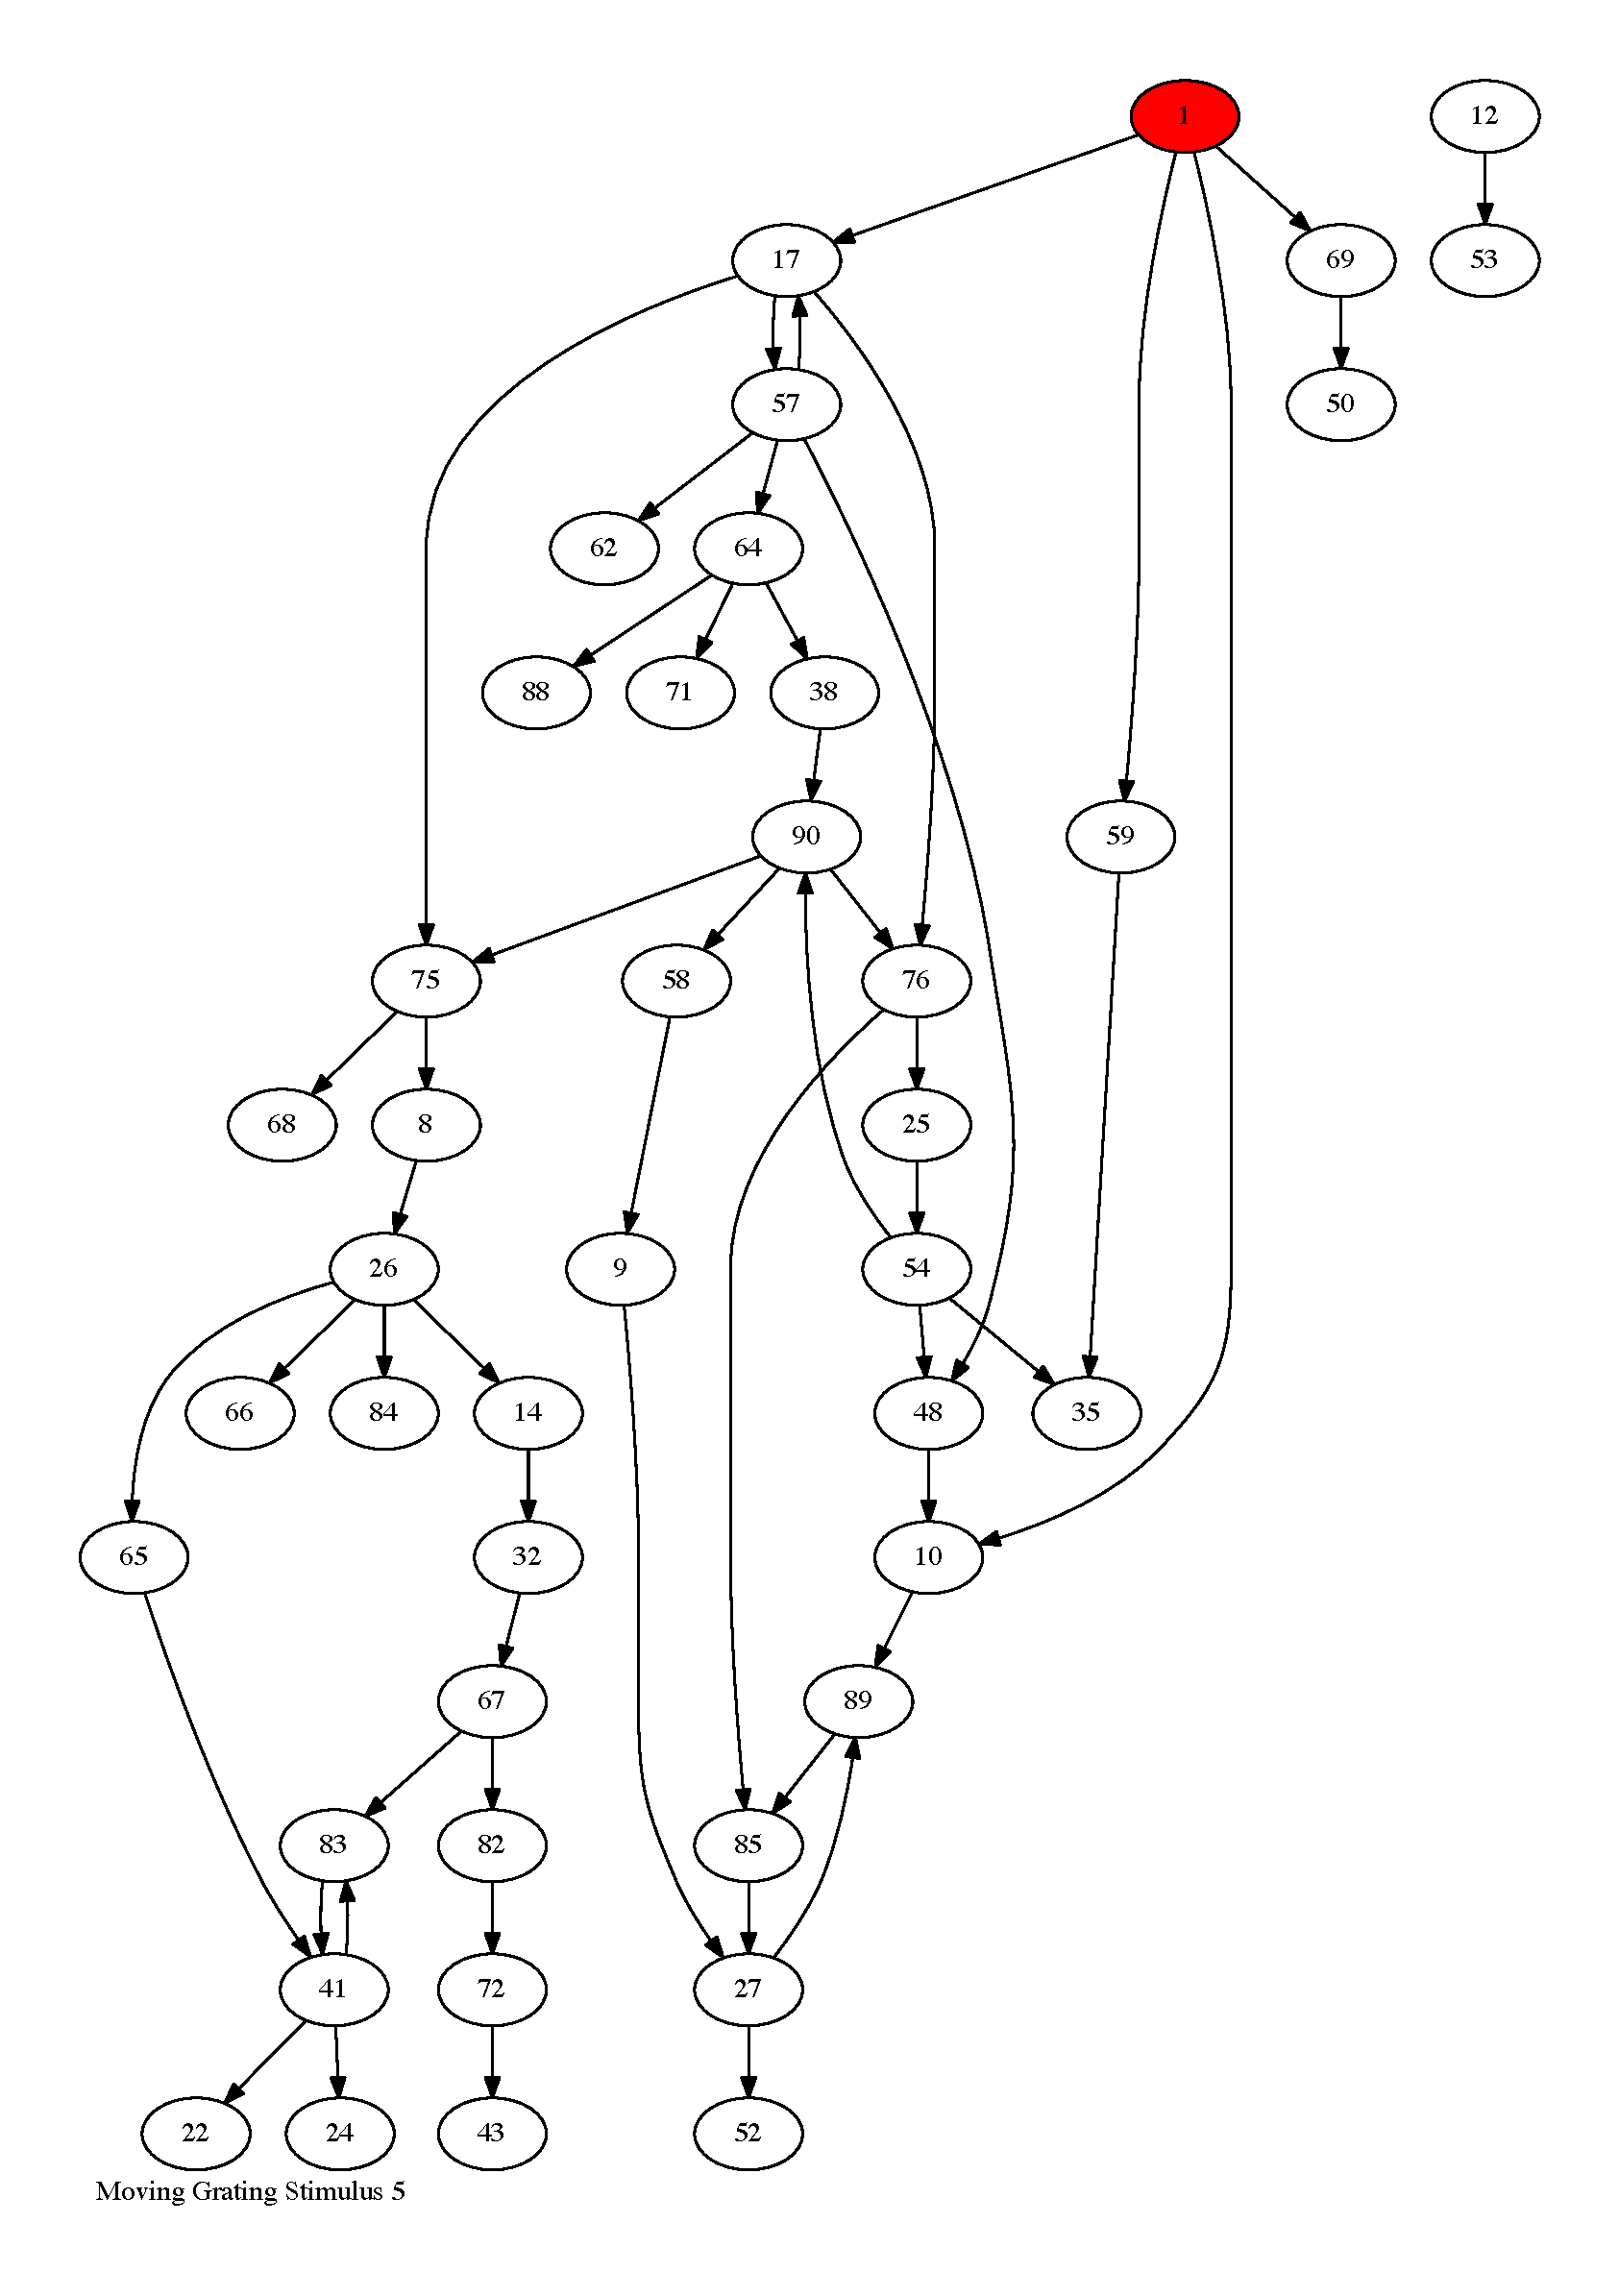
\includegraphics[max height=\textheight,max width=\textwidth]{stim_mov_grat/stim5_pp.pdf}

\newpage
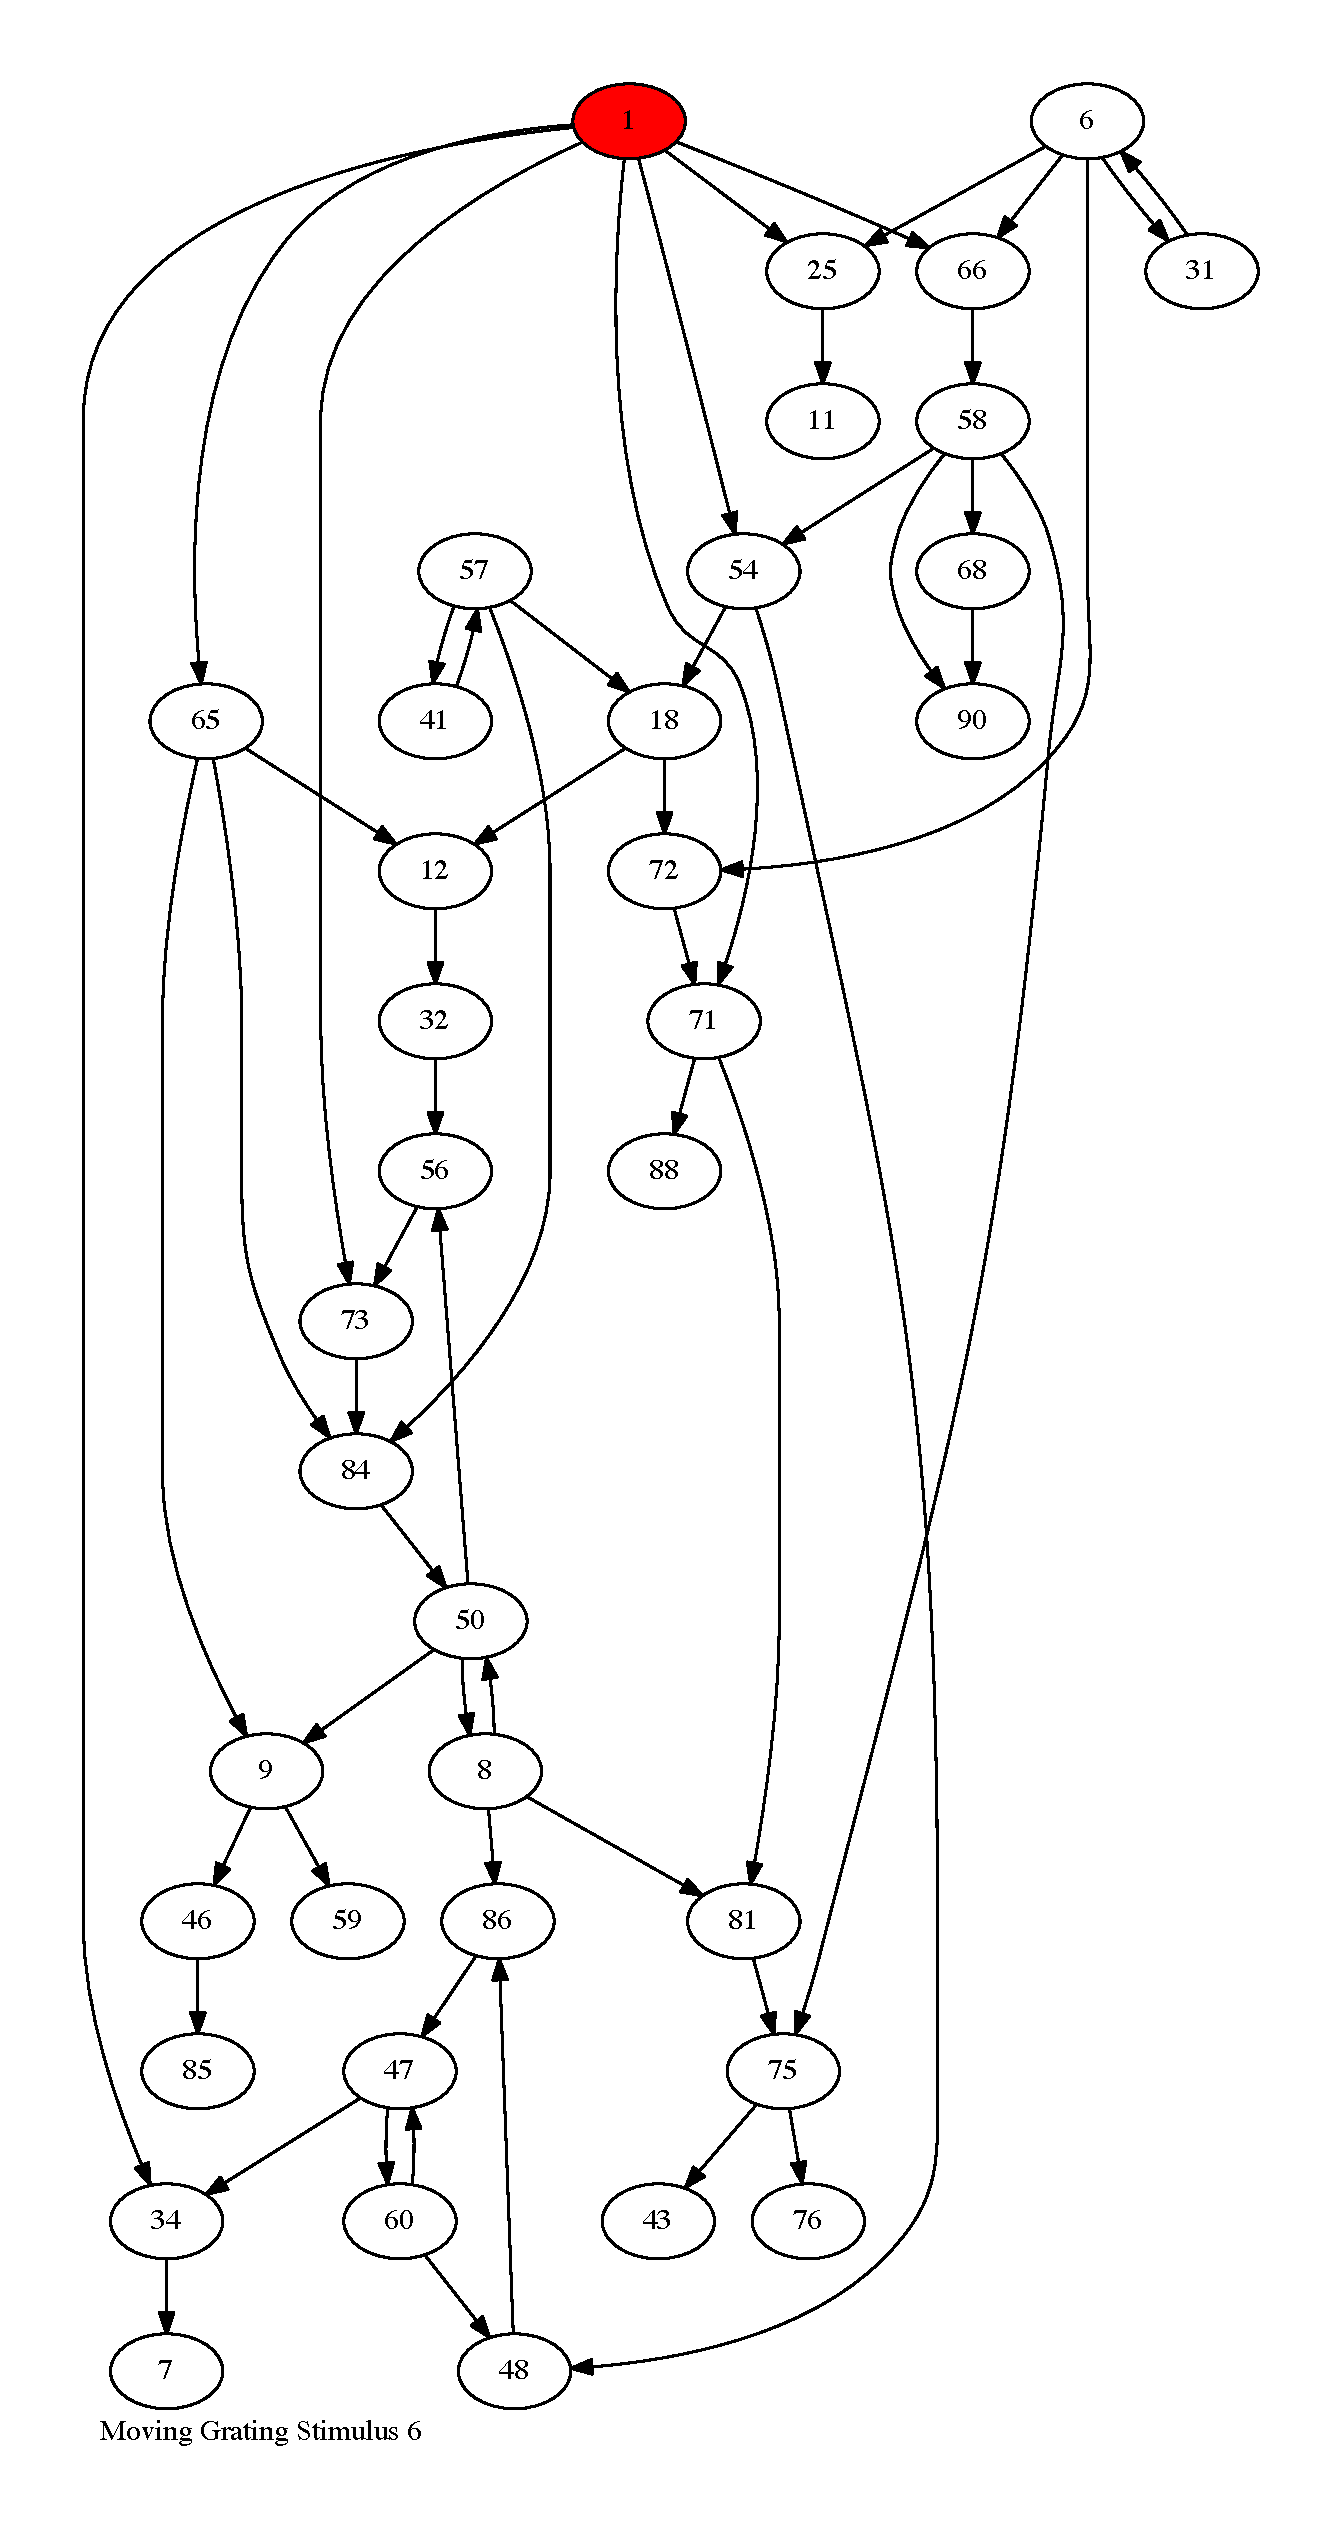
\includegraphics[max height=\textheight,max width=\textwidth]{stim_mov_grat/stim6_pp.pdf}

\newpage
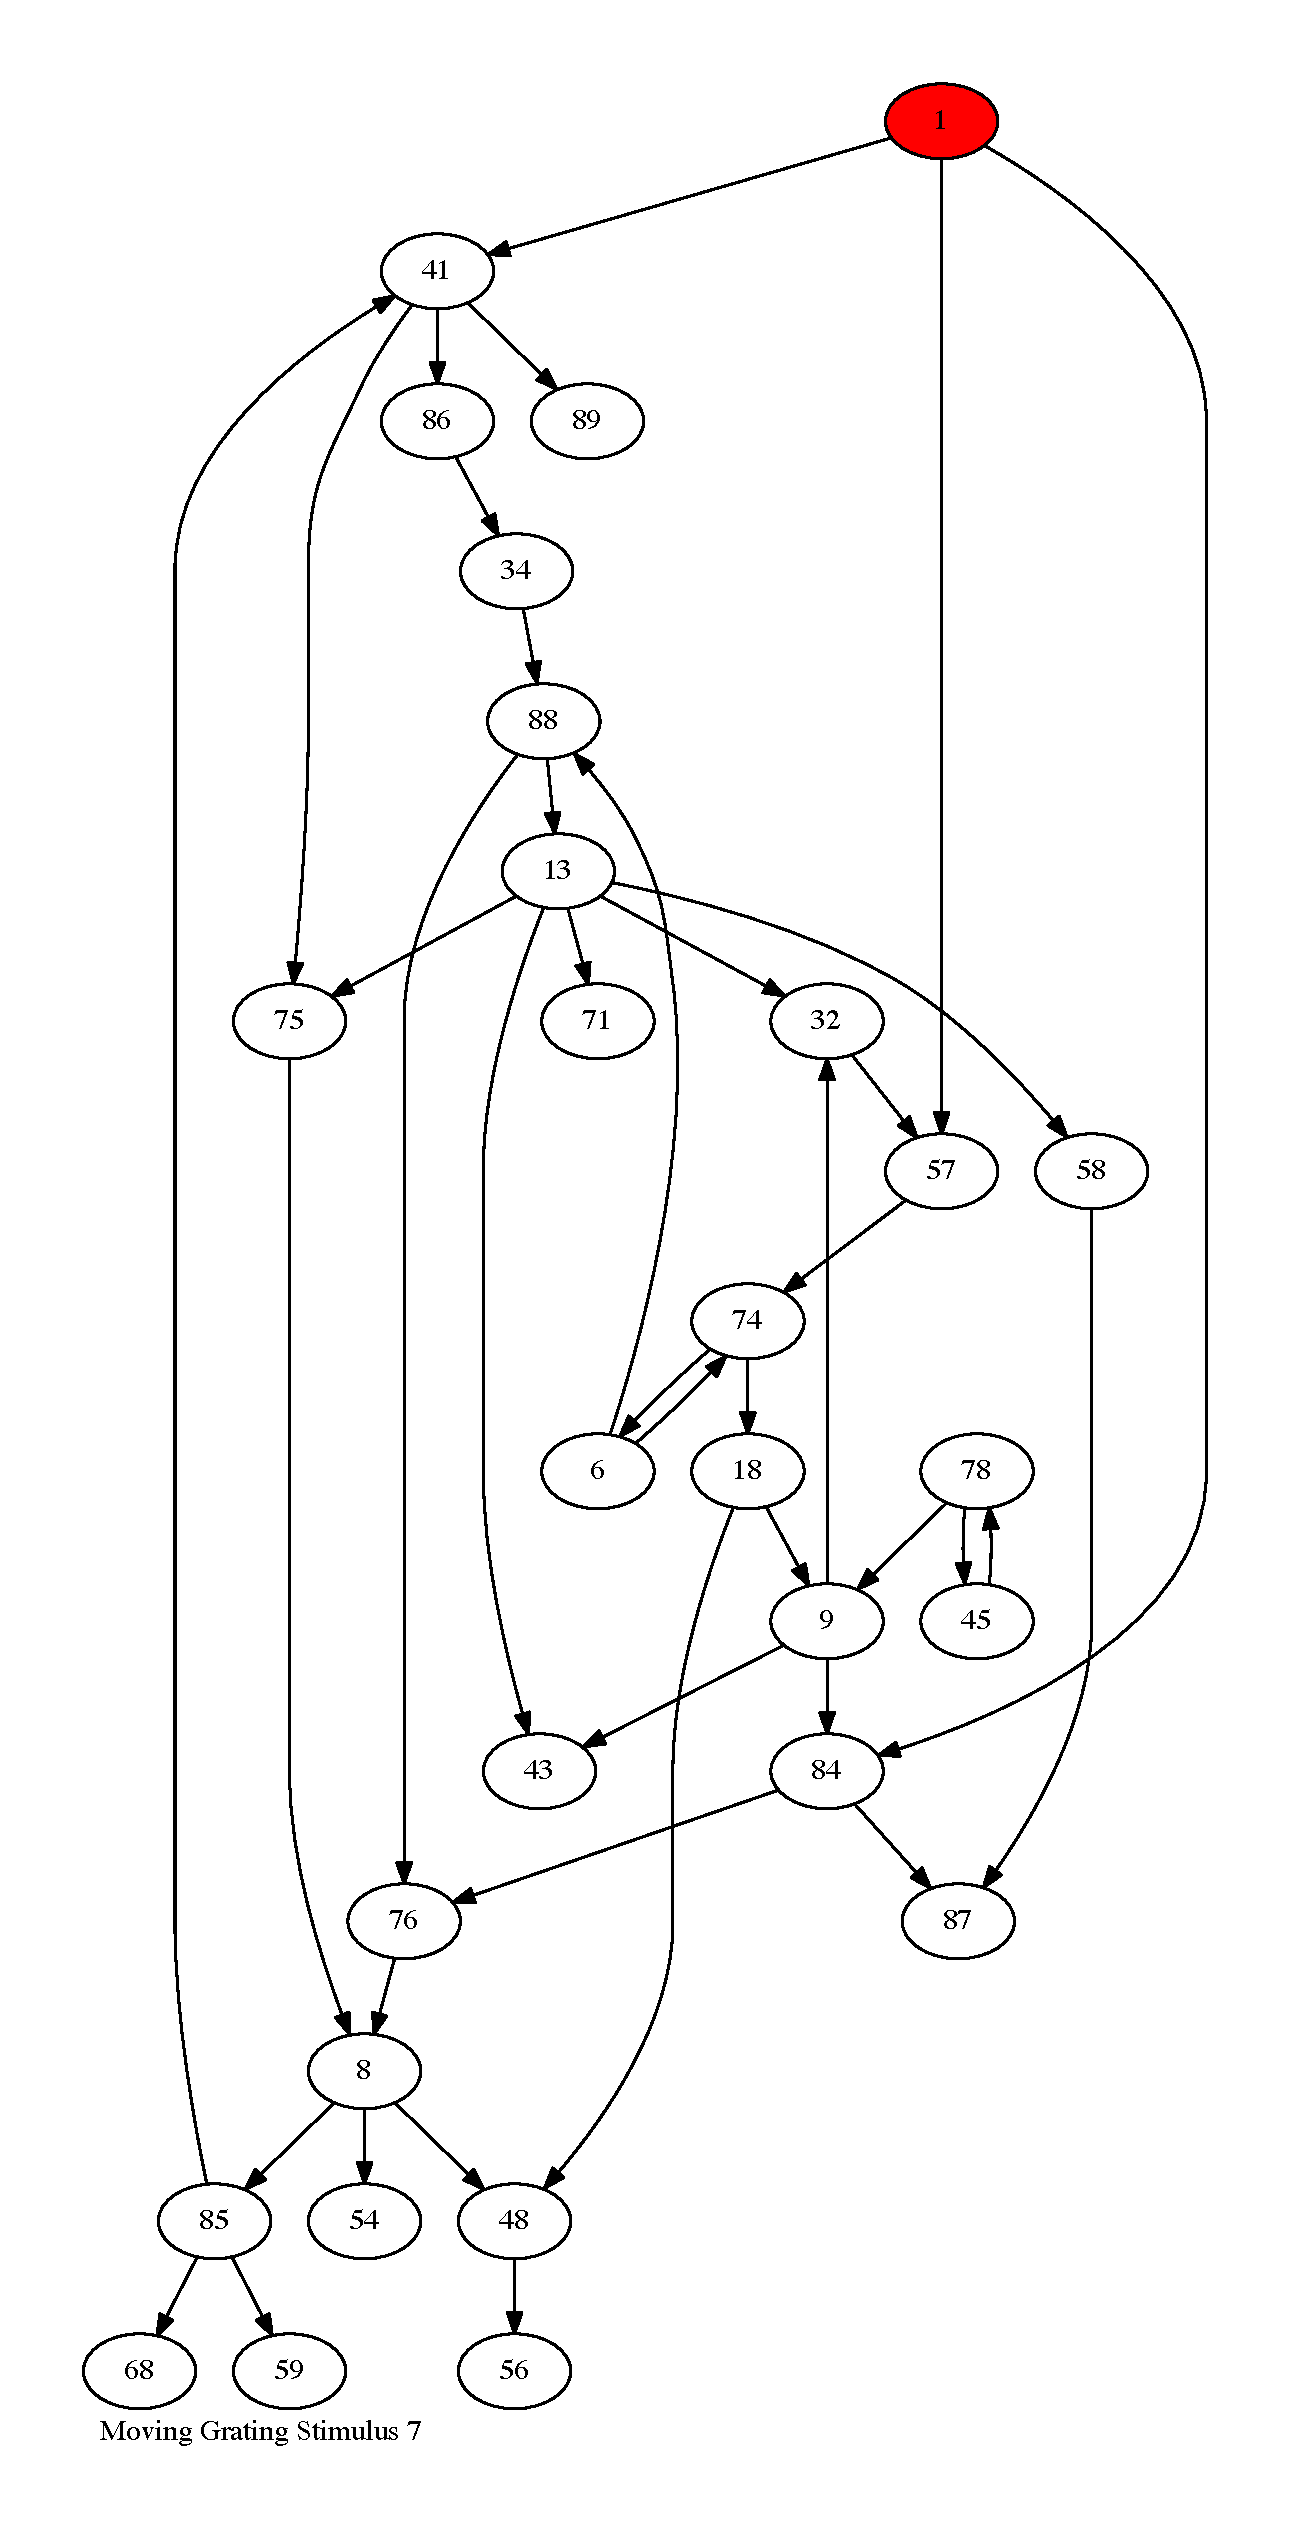
\includegraphics[max height=\textheight,max width=\textwidth]{stim_mov_grat/stim7_pp.pdf}

\newpage
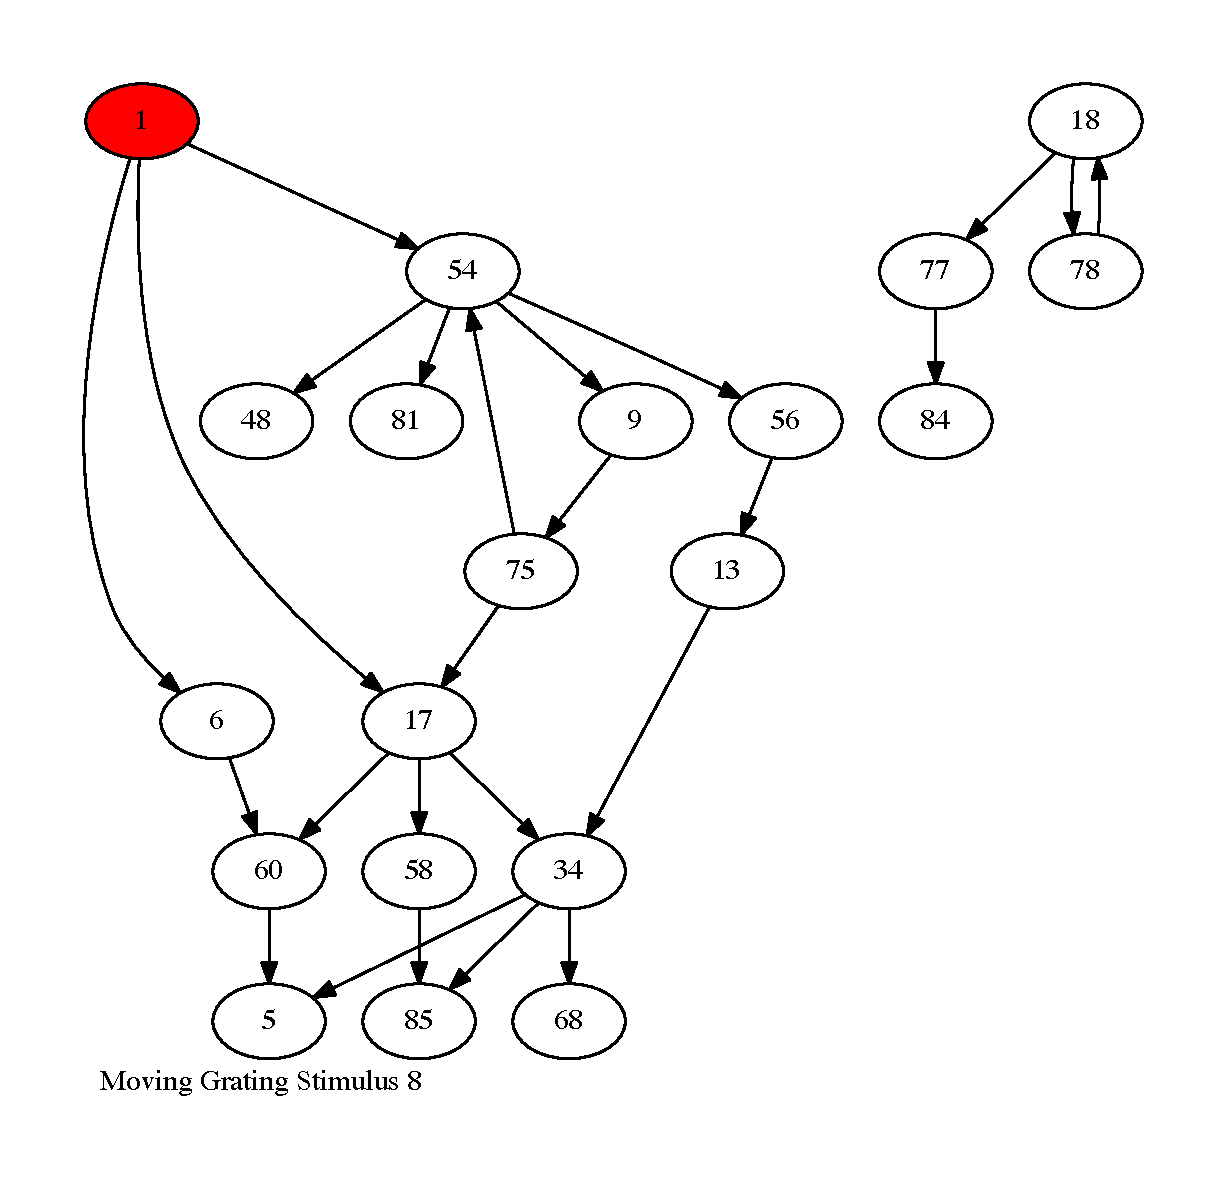
\includegraphics[max height=\textheight,max width=\textwidth]{stim_mov_grat/stim8_pp.pdf}

\newpage
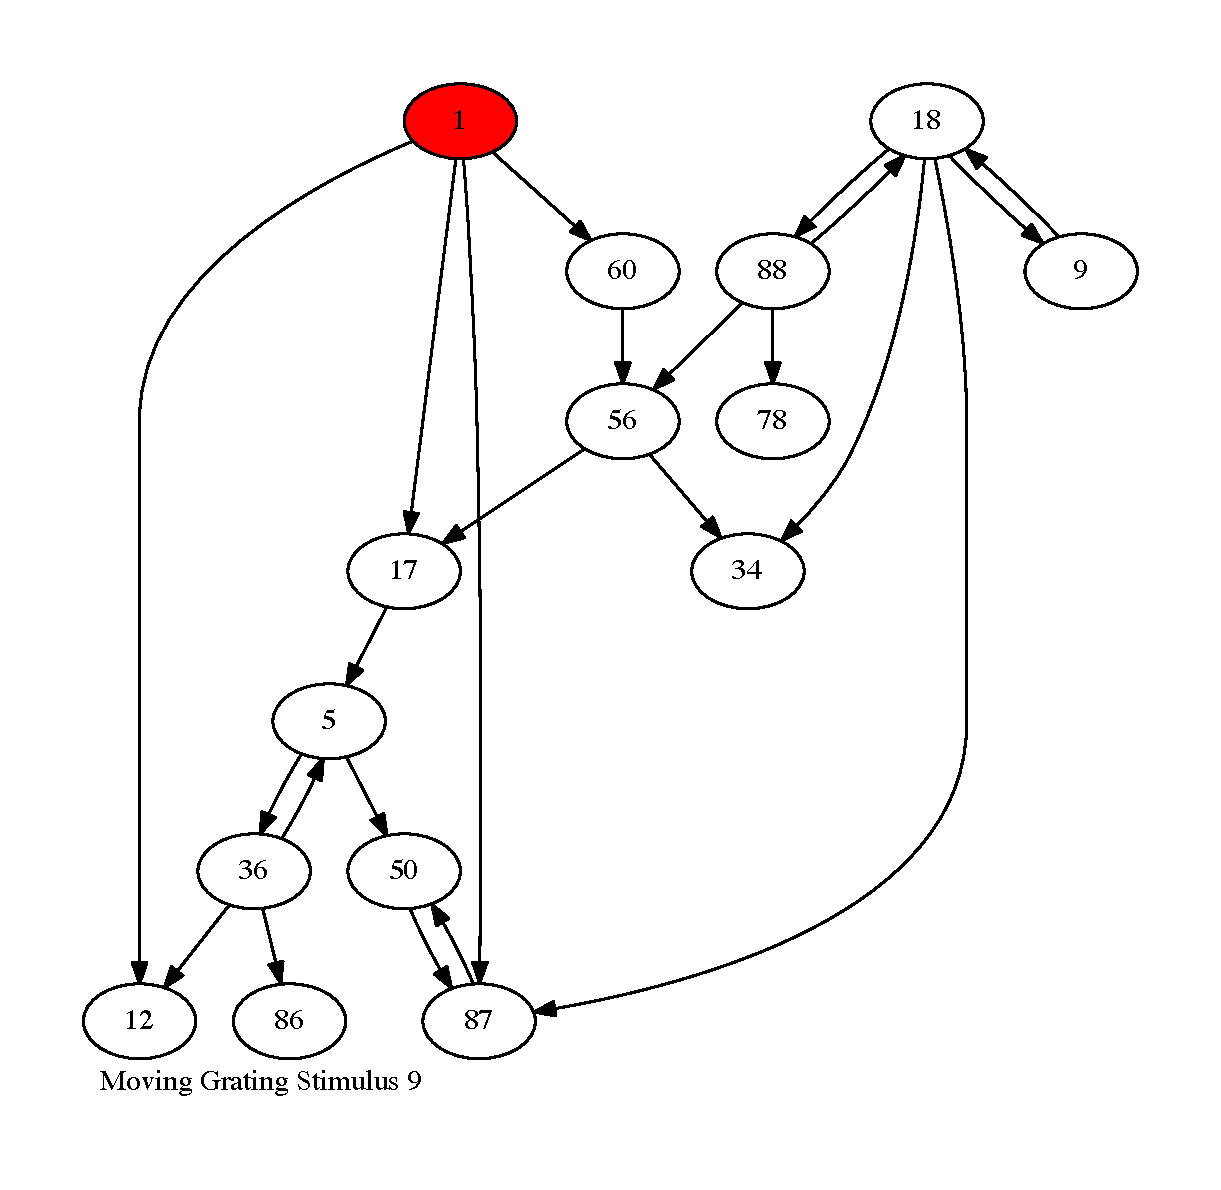
\includegraphics[max height=\textheight,max width=\textwidth]{stim_mov_grat/stim9_pp.pdf}

\newpage
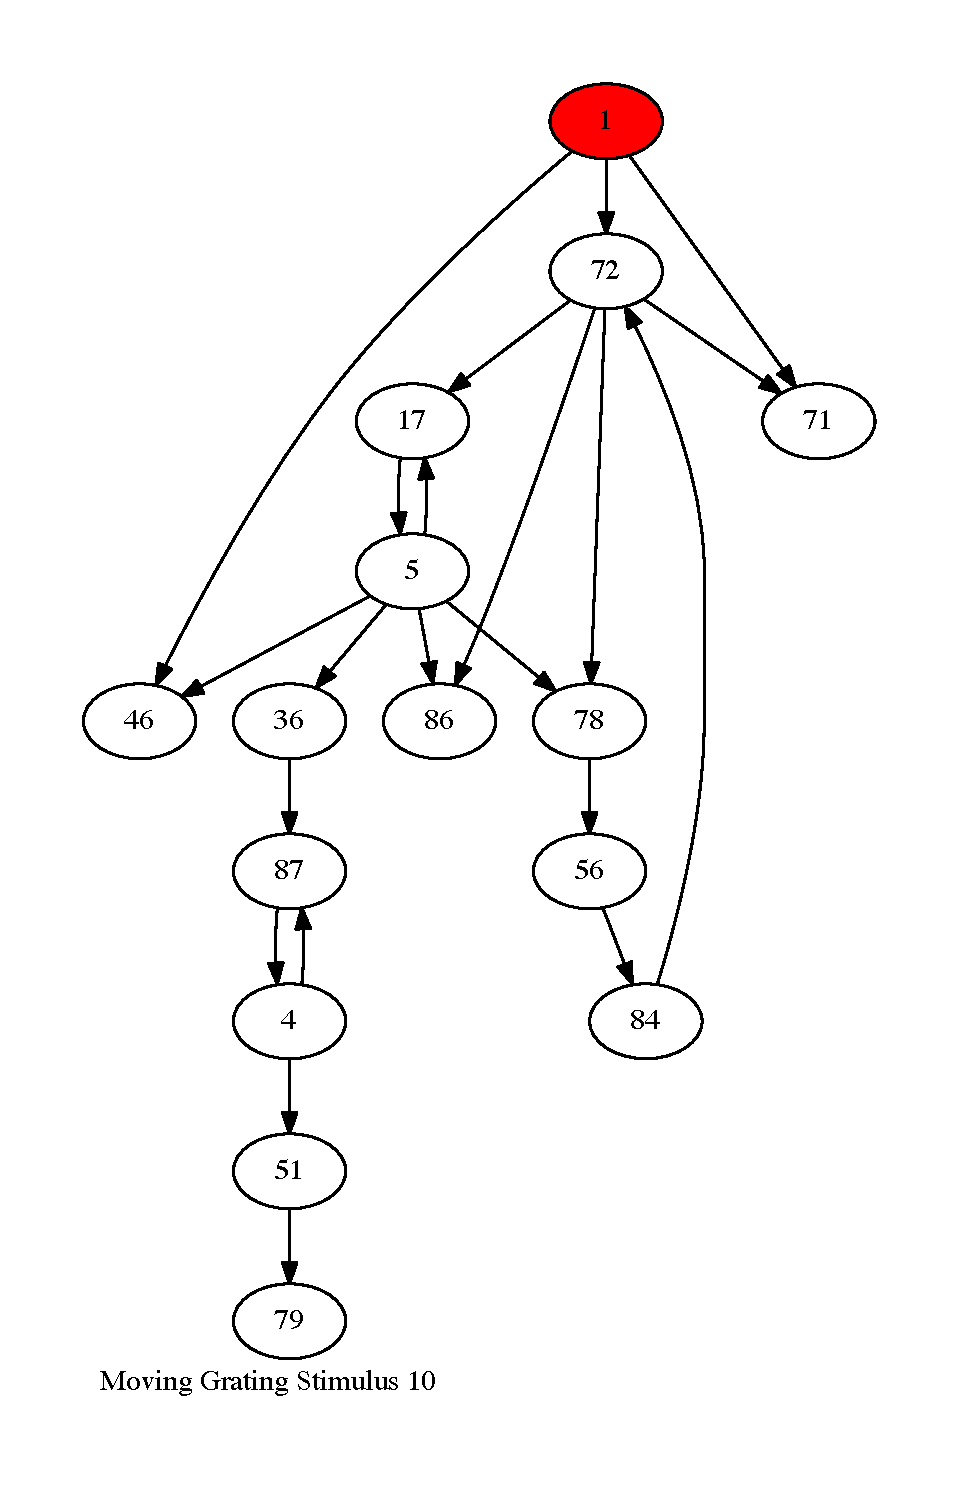
\includegraphics[max height=\textheight,max width=\textwidth]{stim_mov_grat/stim10_pp.pdf}

\newpage
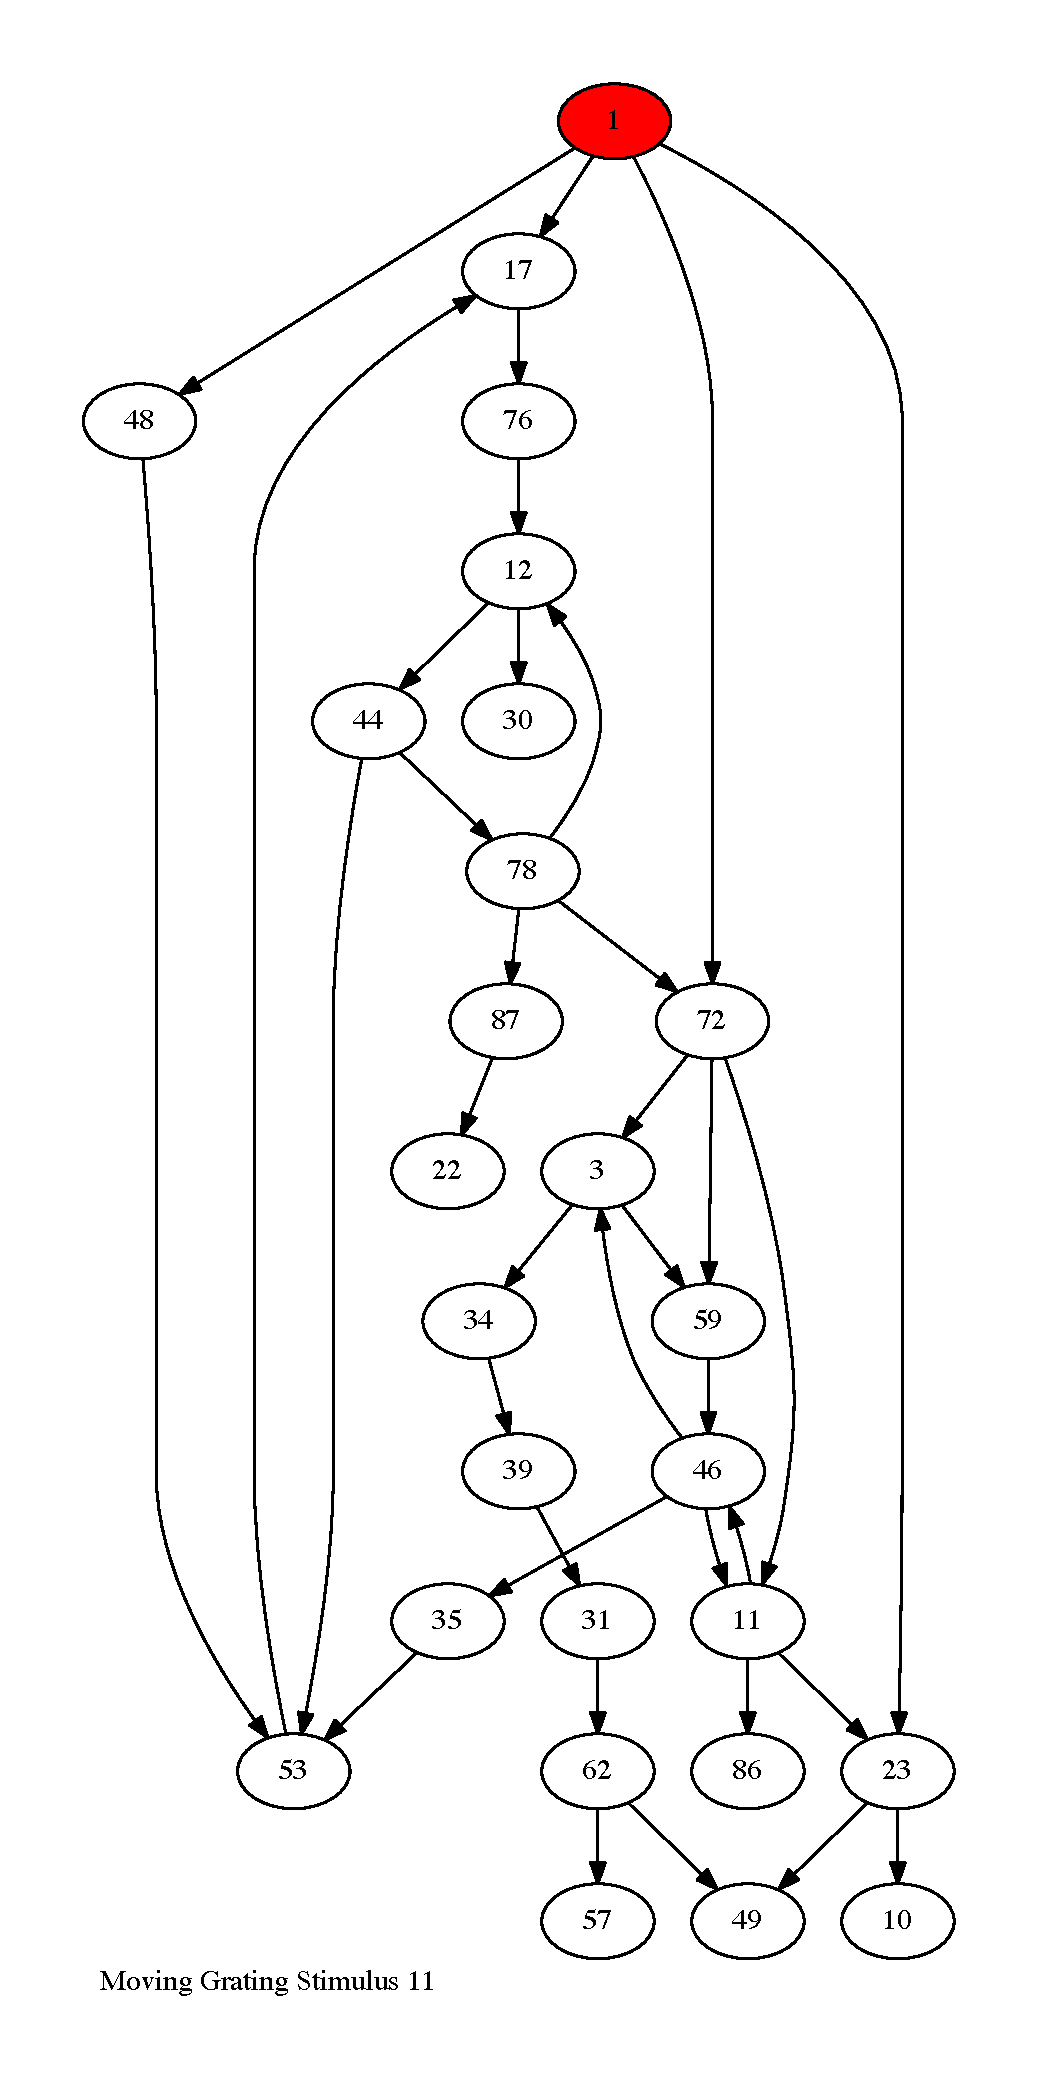
\includegraphics[max height=\textheight,max width=\textwidth]{stim_mov_grat/stim11_pp.pdf}

\newpage
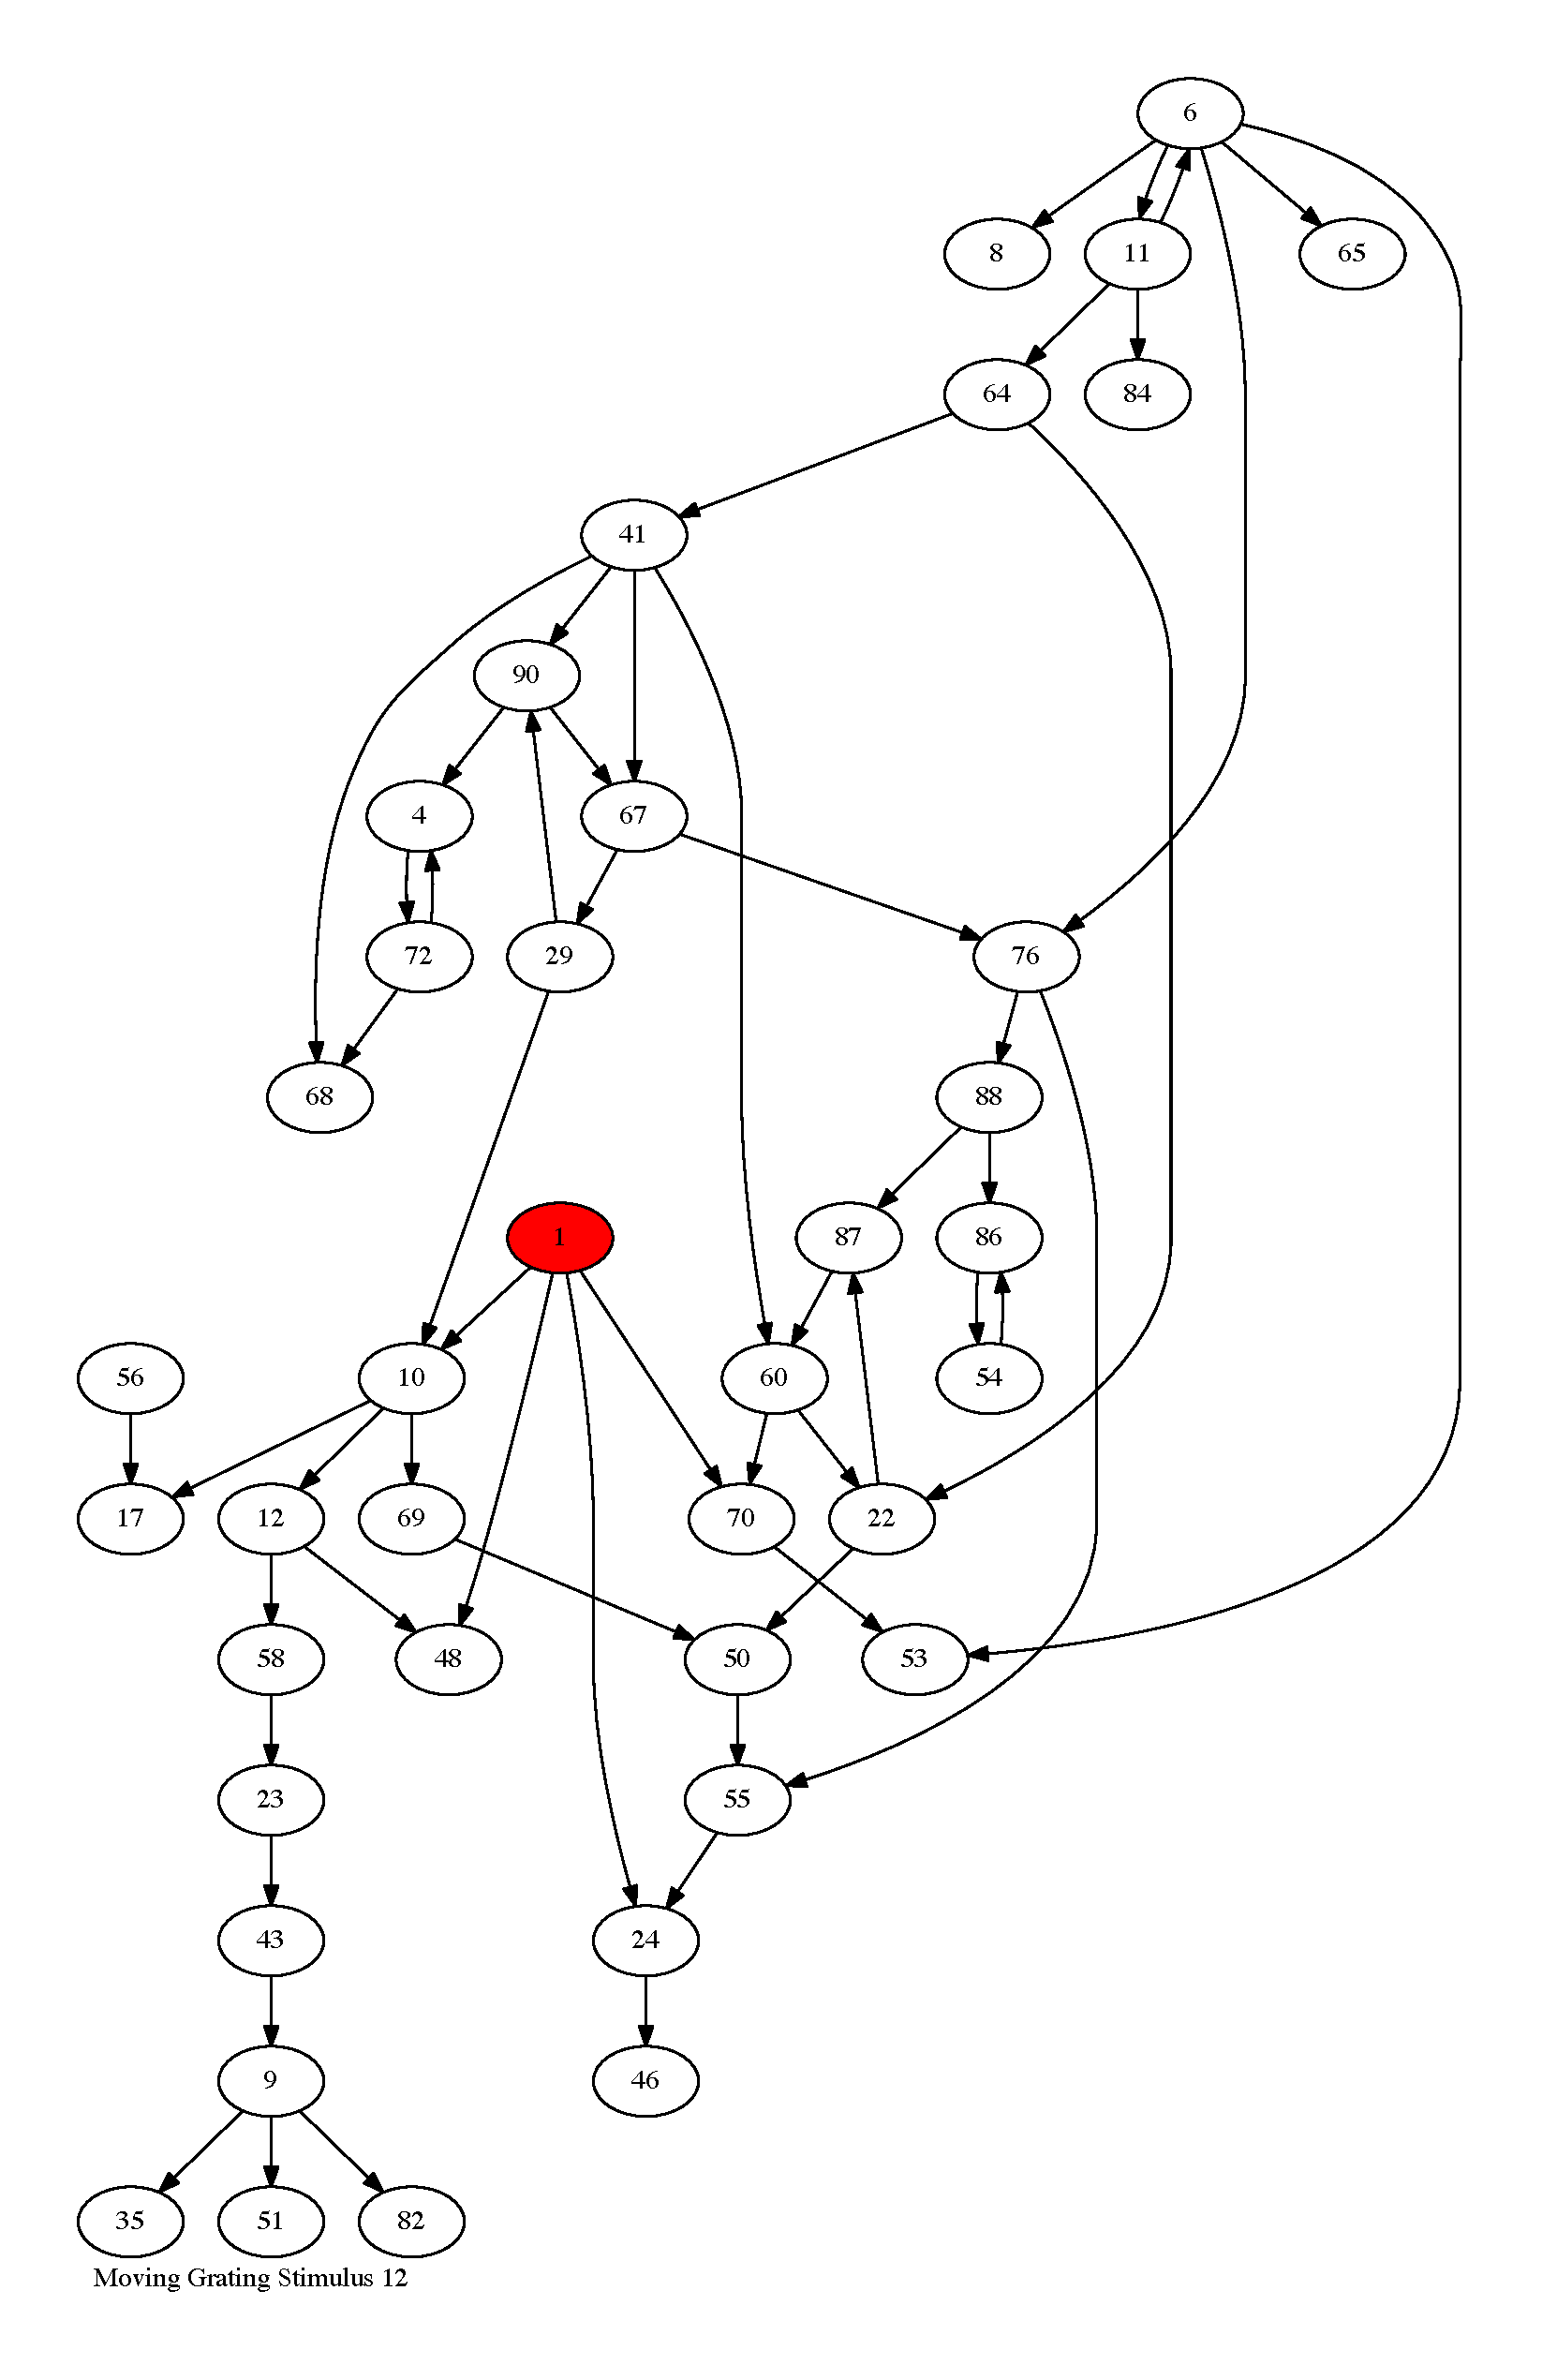
\includegraphics[max height=\textheight,max width=\textwidth]{stim_mov_grat/stim12_pp.pdf}

\newpage
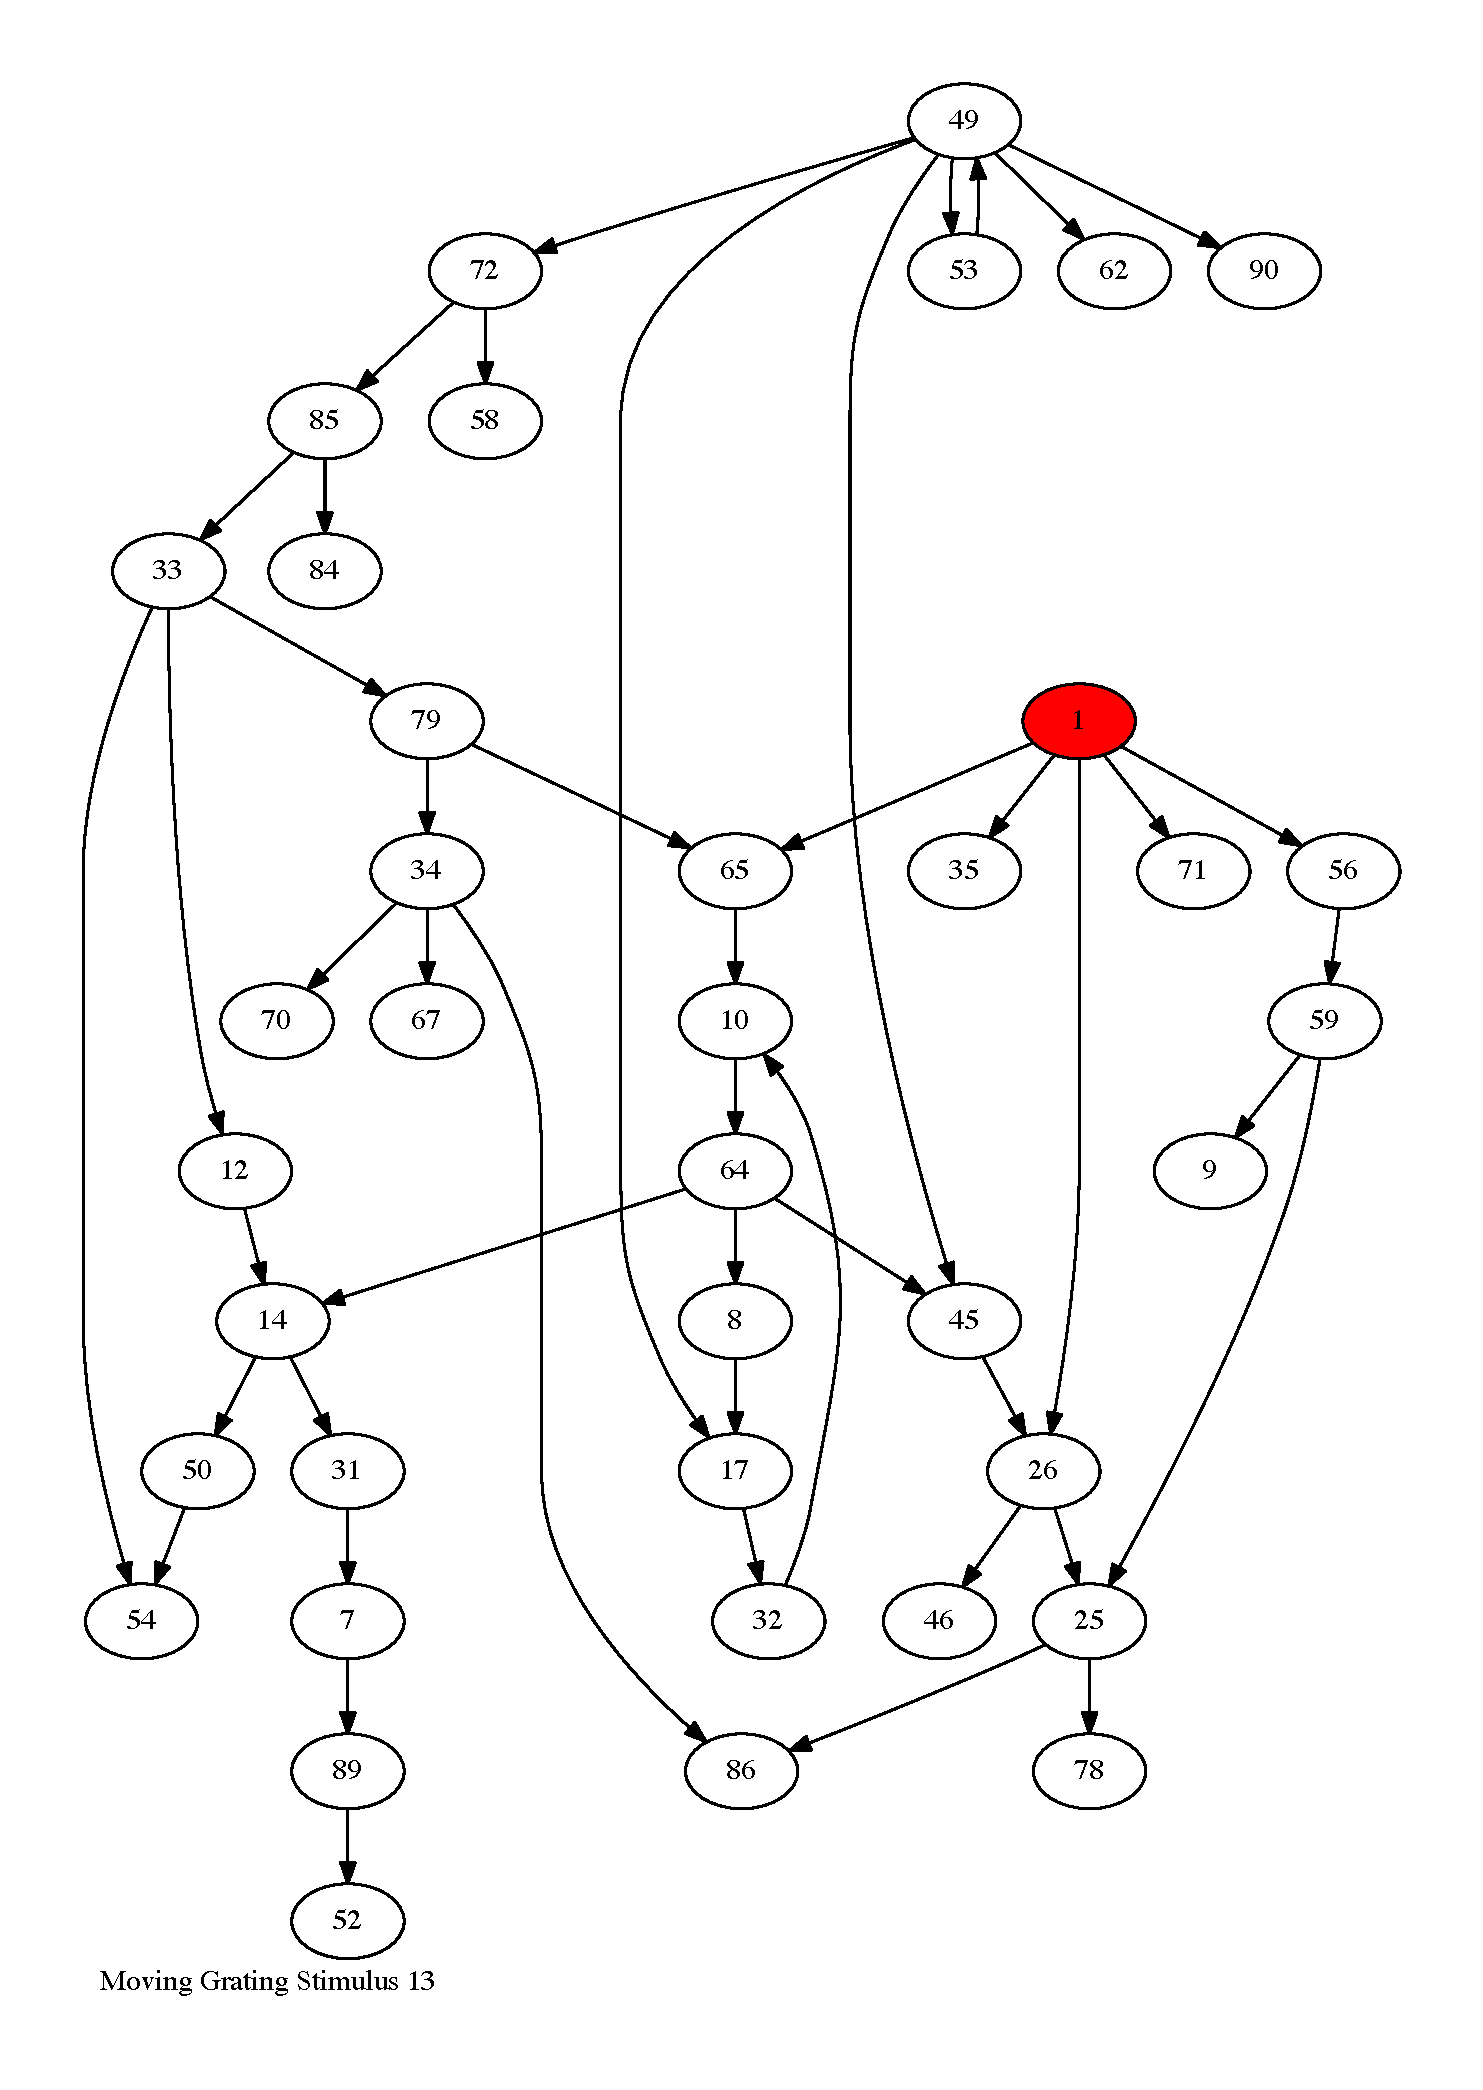
\includegraphics[max height=\textheight,max width=\textwidth]{stim_mov_grat/stim13_pp.pdf}

\newpage
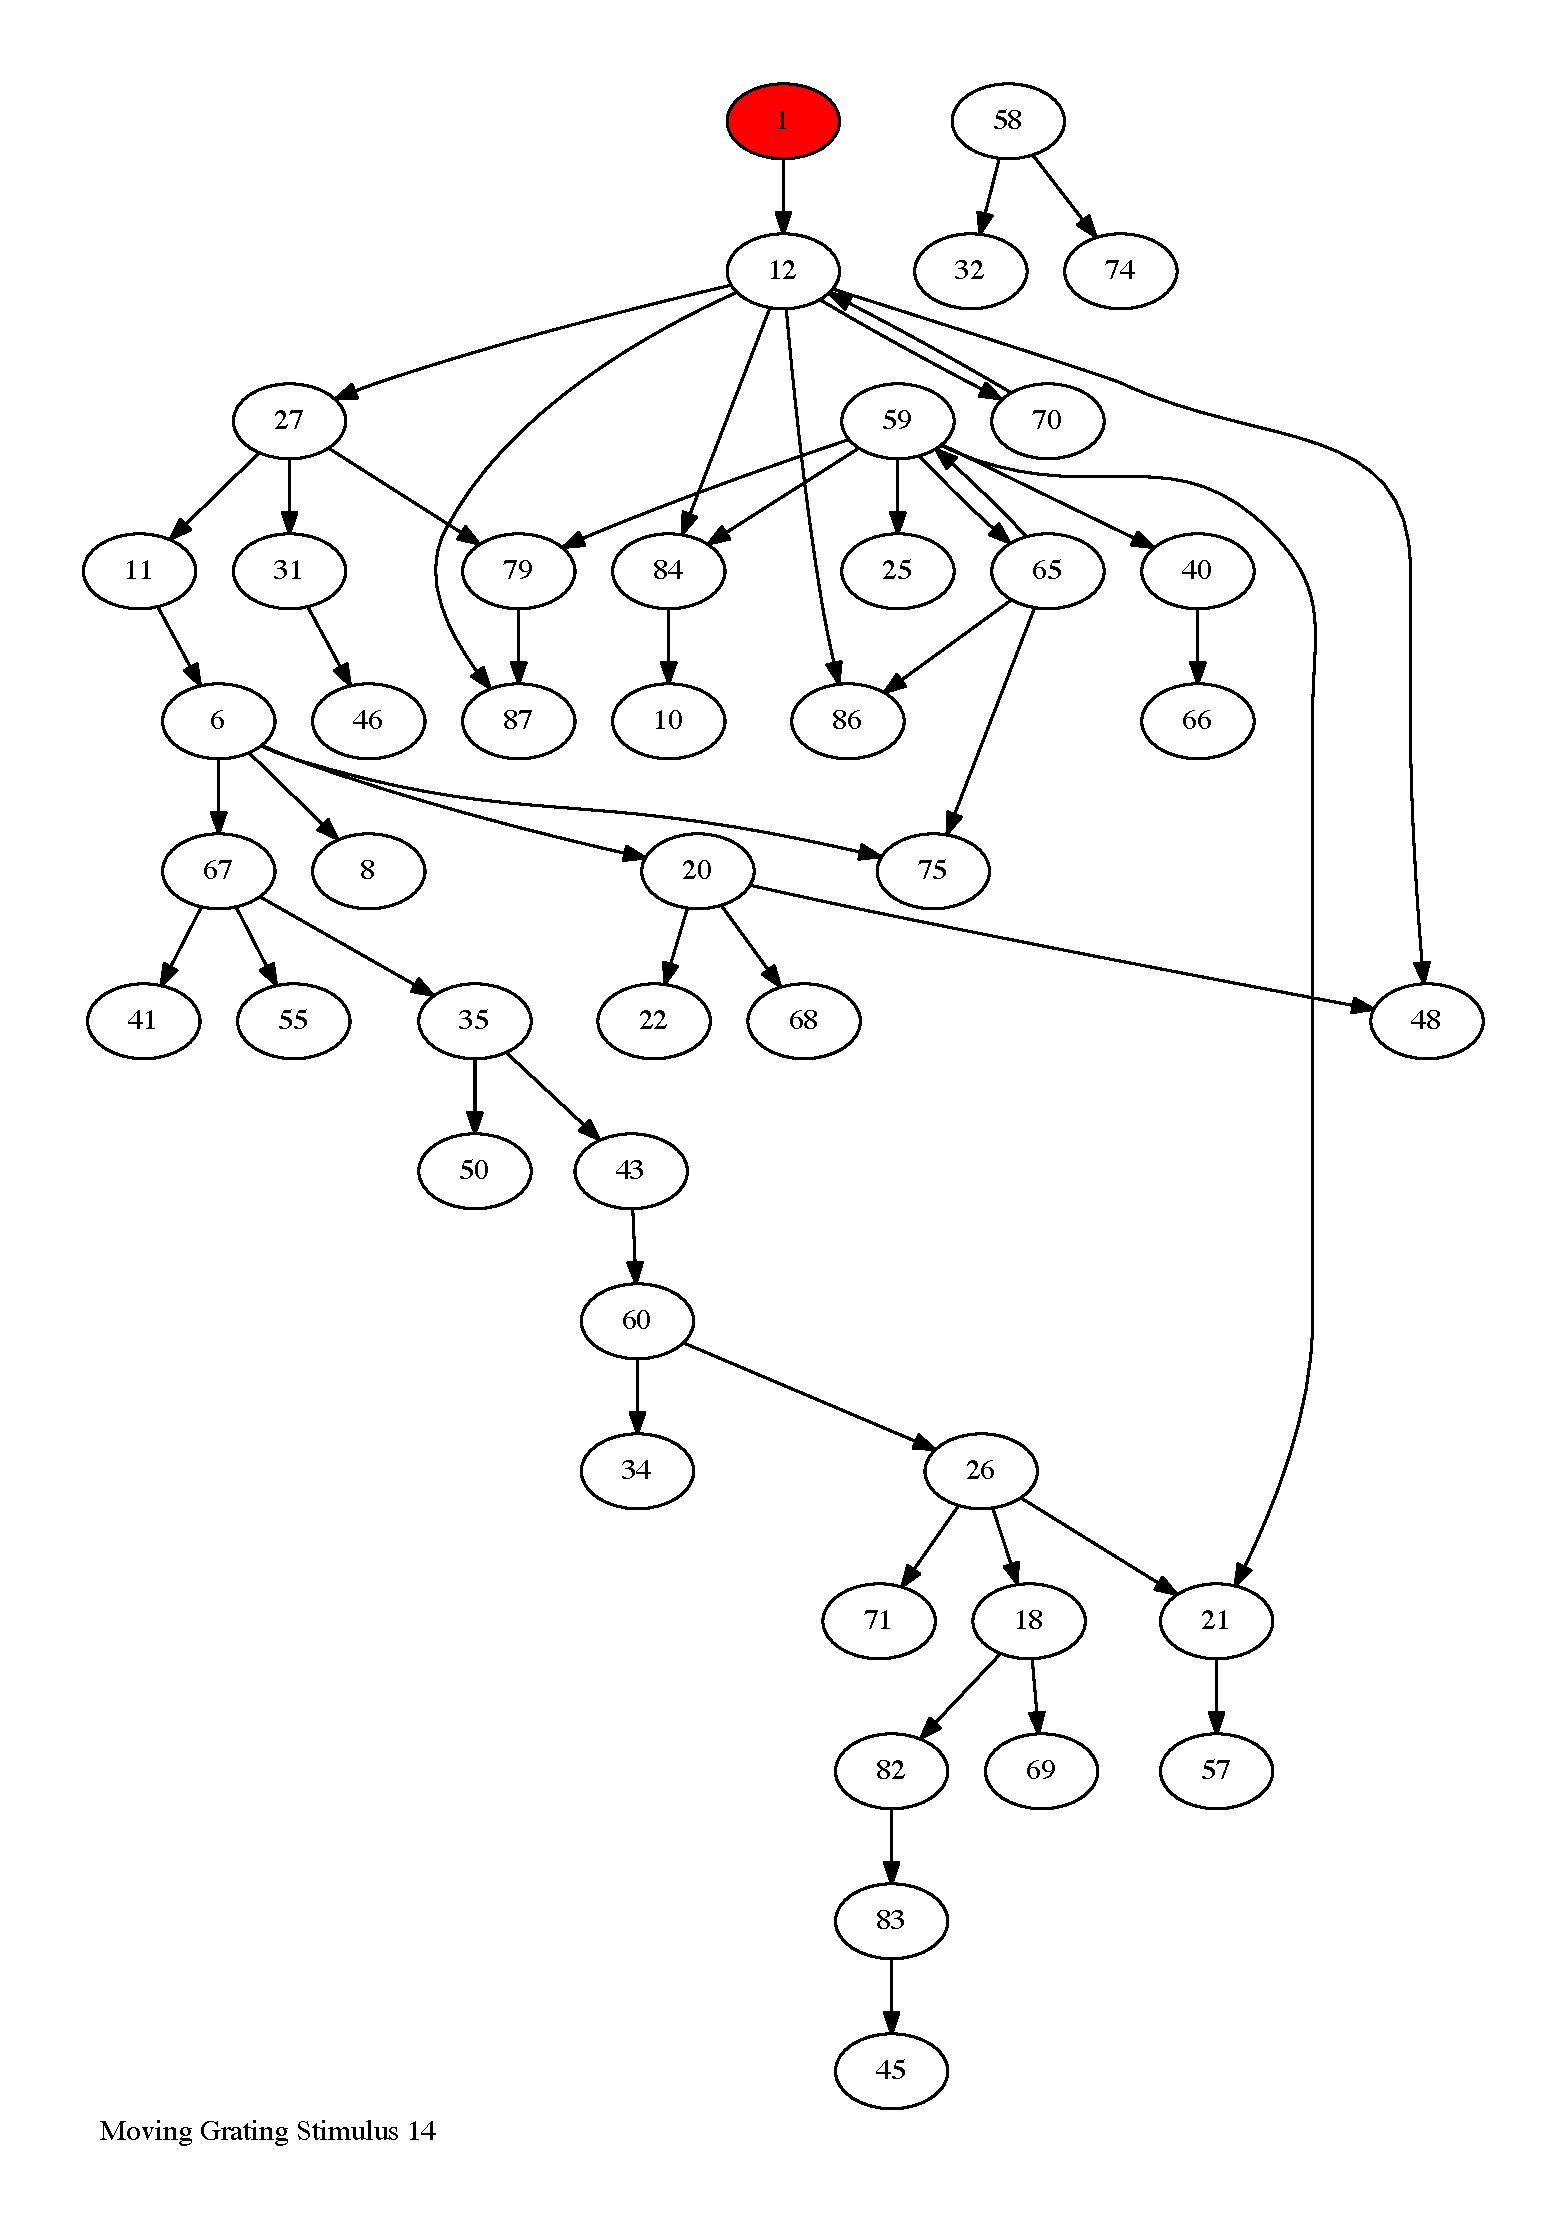
\includegraphics[max height=\textheight,max width=\textwidth]{stim_mov_grat/stim14_pp.pdf}

\newpage
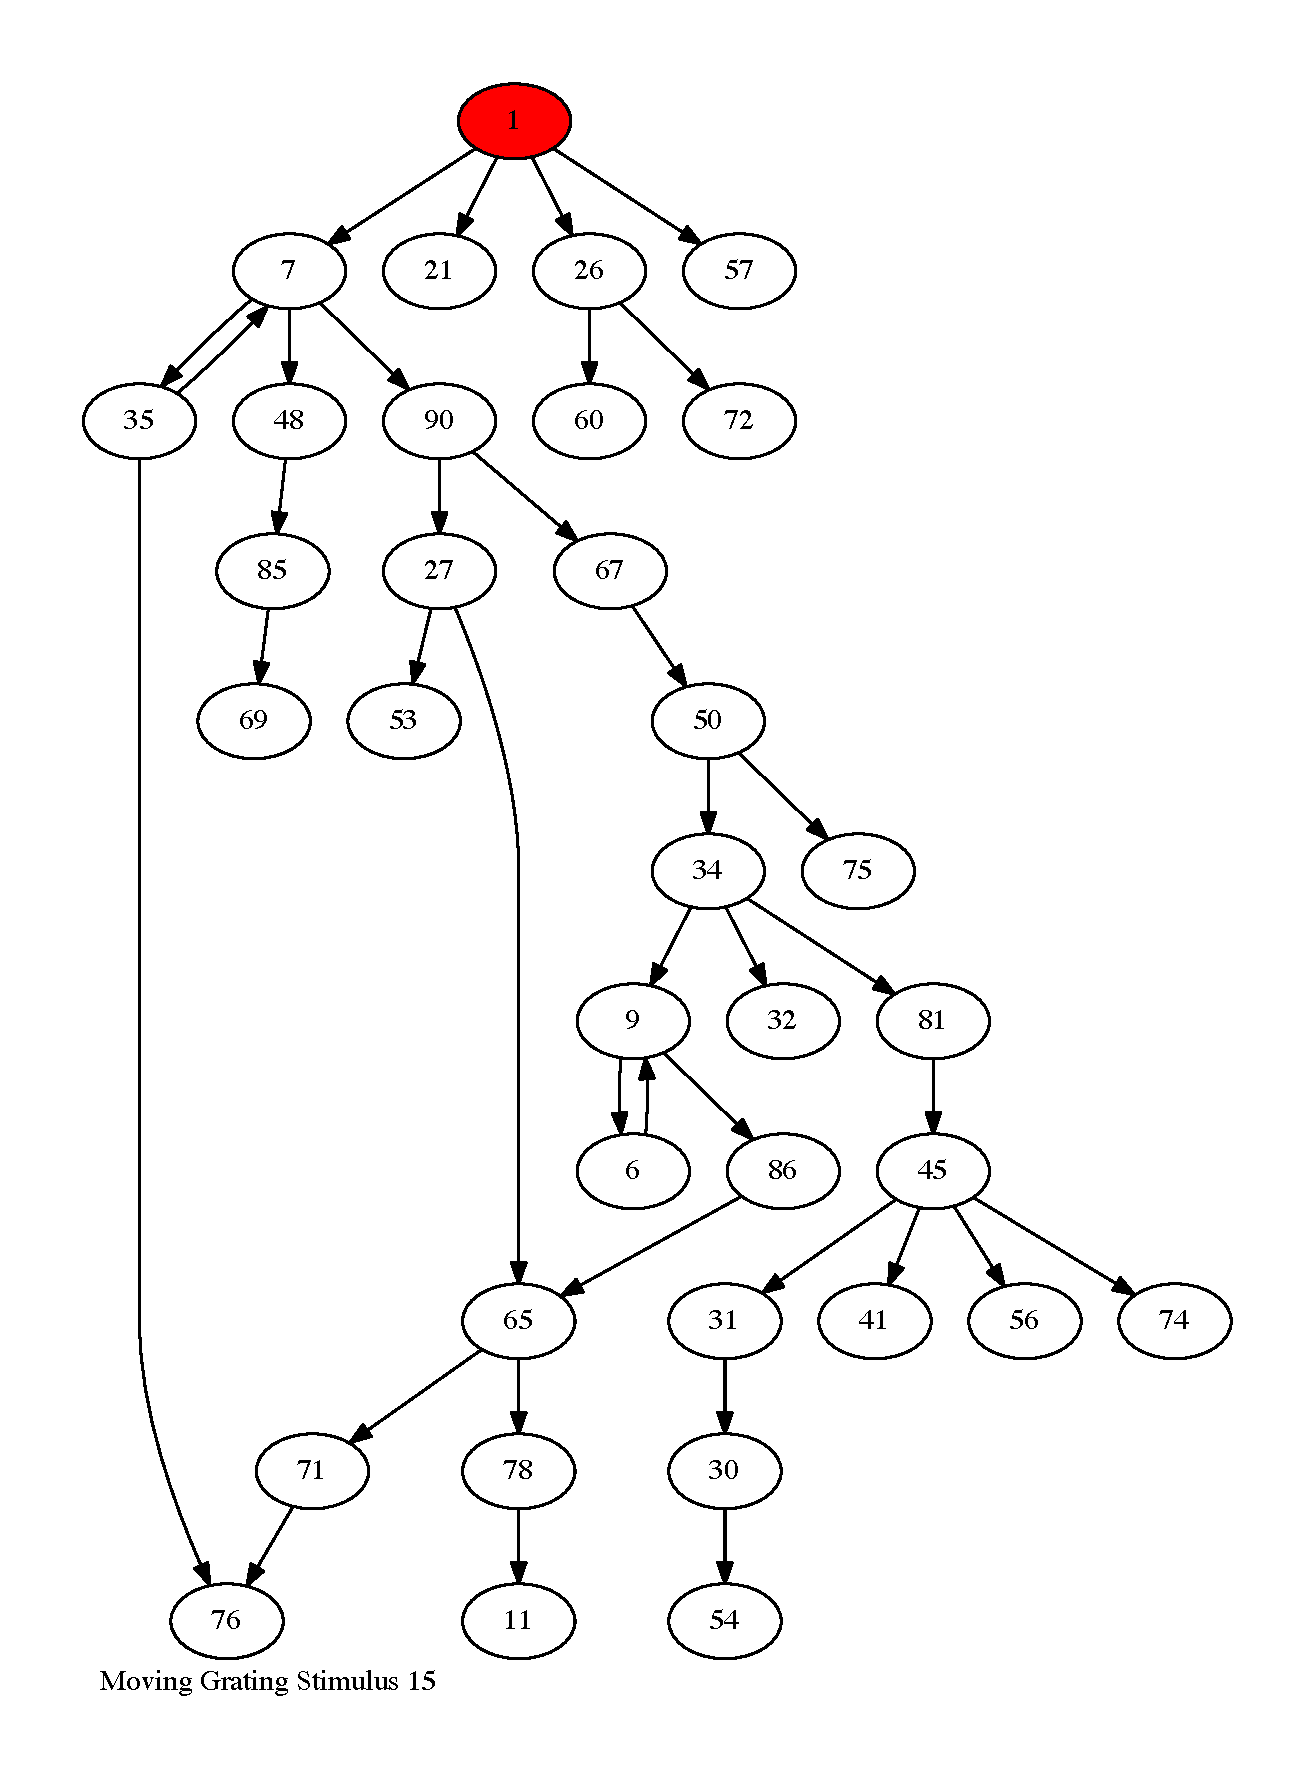
\includegraphics[max height=\textheight,max width=\textwidth]{stim_mov_grat/stim15_pp.pdf}

\newpage
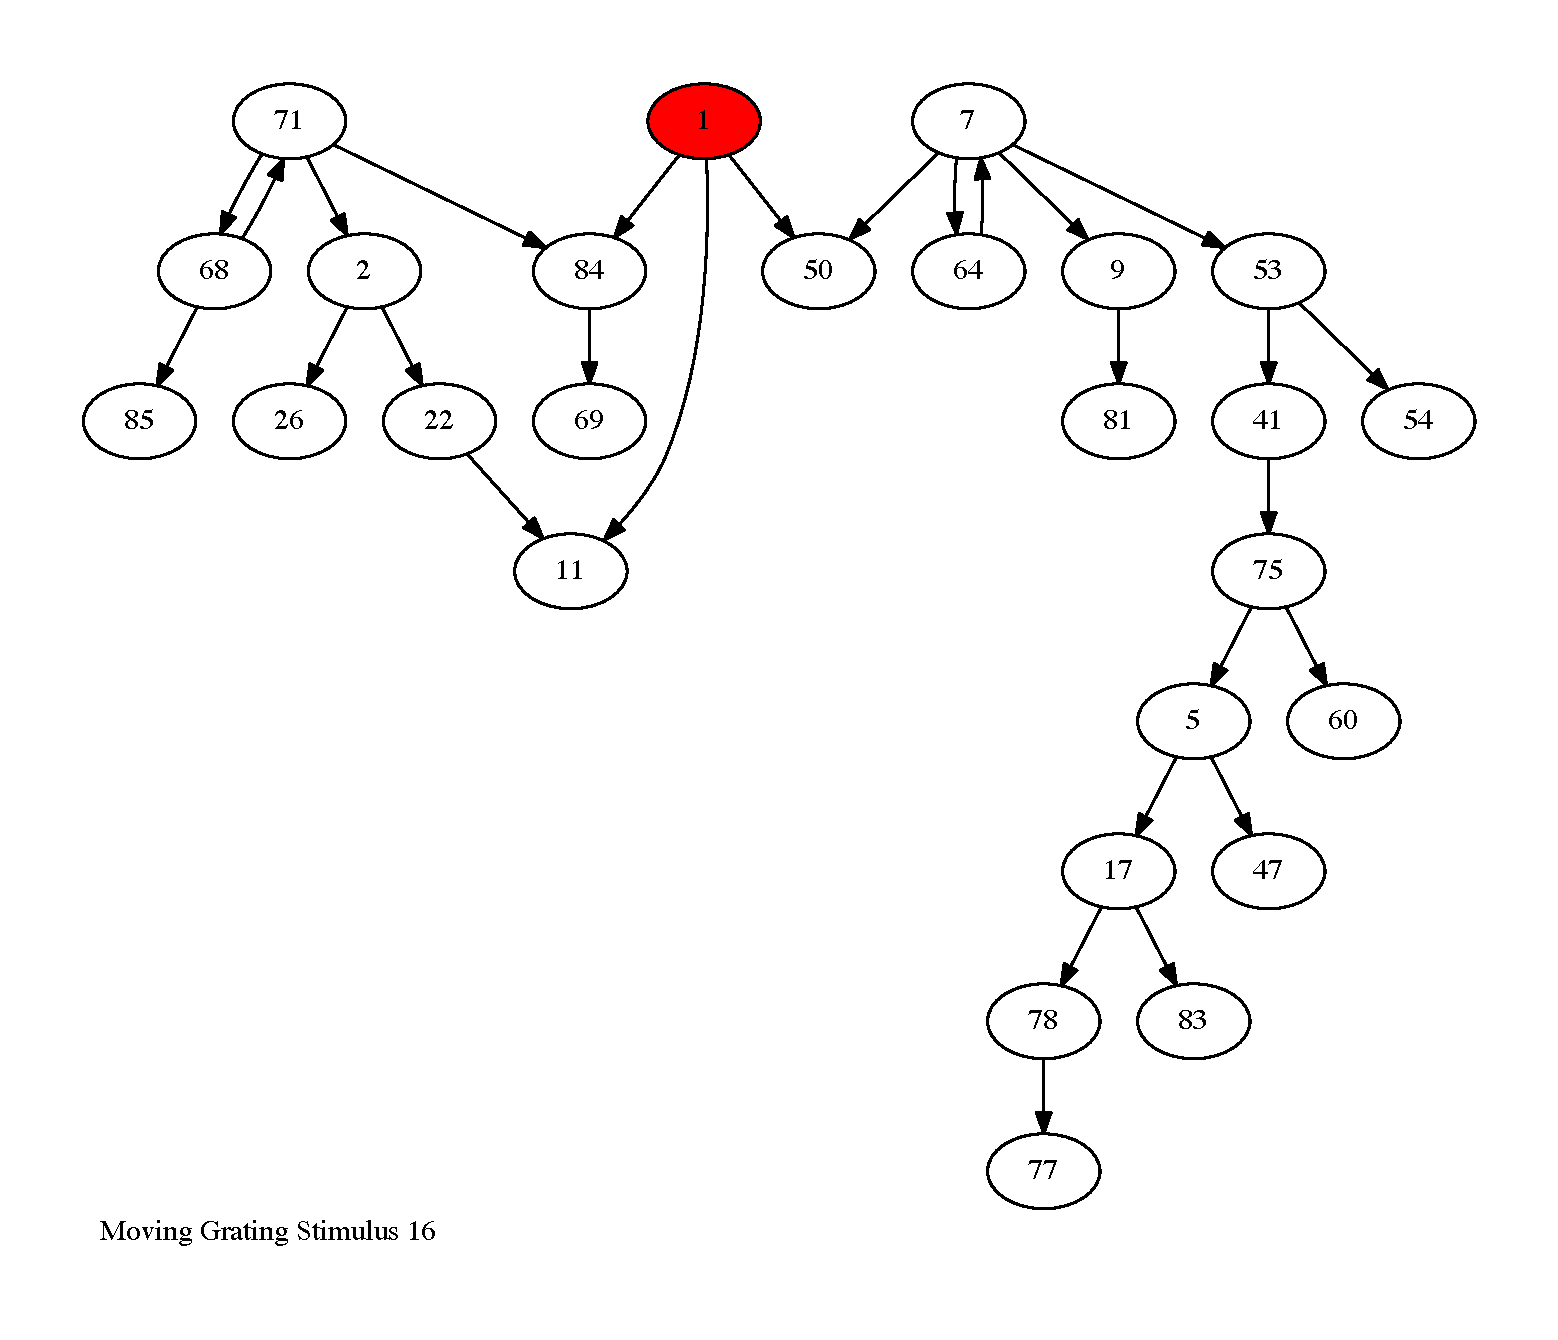
\includegraphics[max height=\textheight,max width=\textwidth]{stim_mov_grat/stim16_pp.pdf}

%%%%%%%%%%%%%%%%%%%%%%%%%%%%%%%% BL LOOMING OBJECTS %%%%%%%%%%%%%%%%%%%%%%%%%%%

\newpage
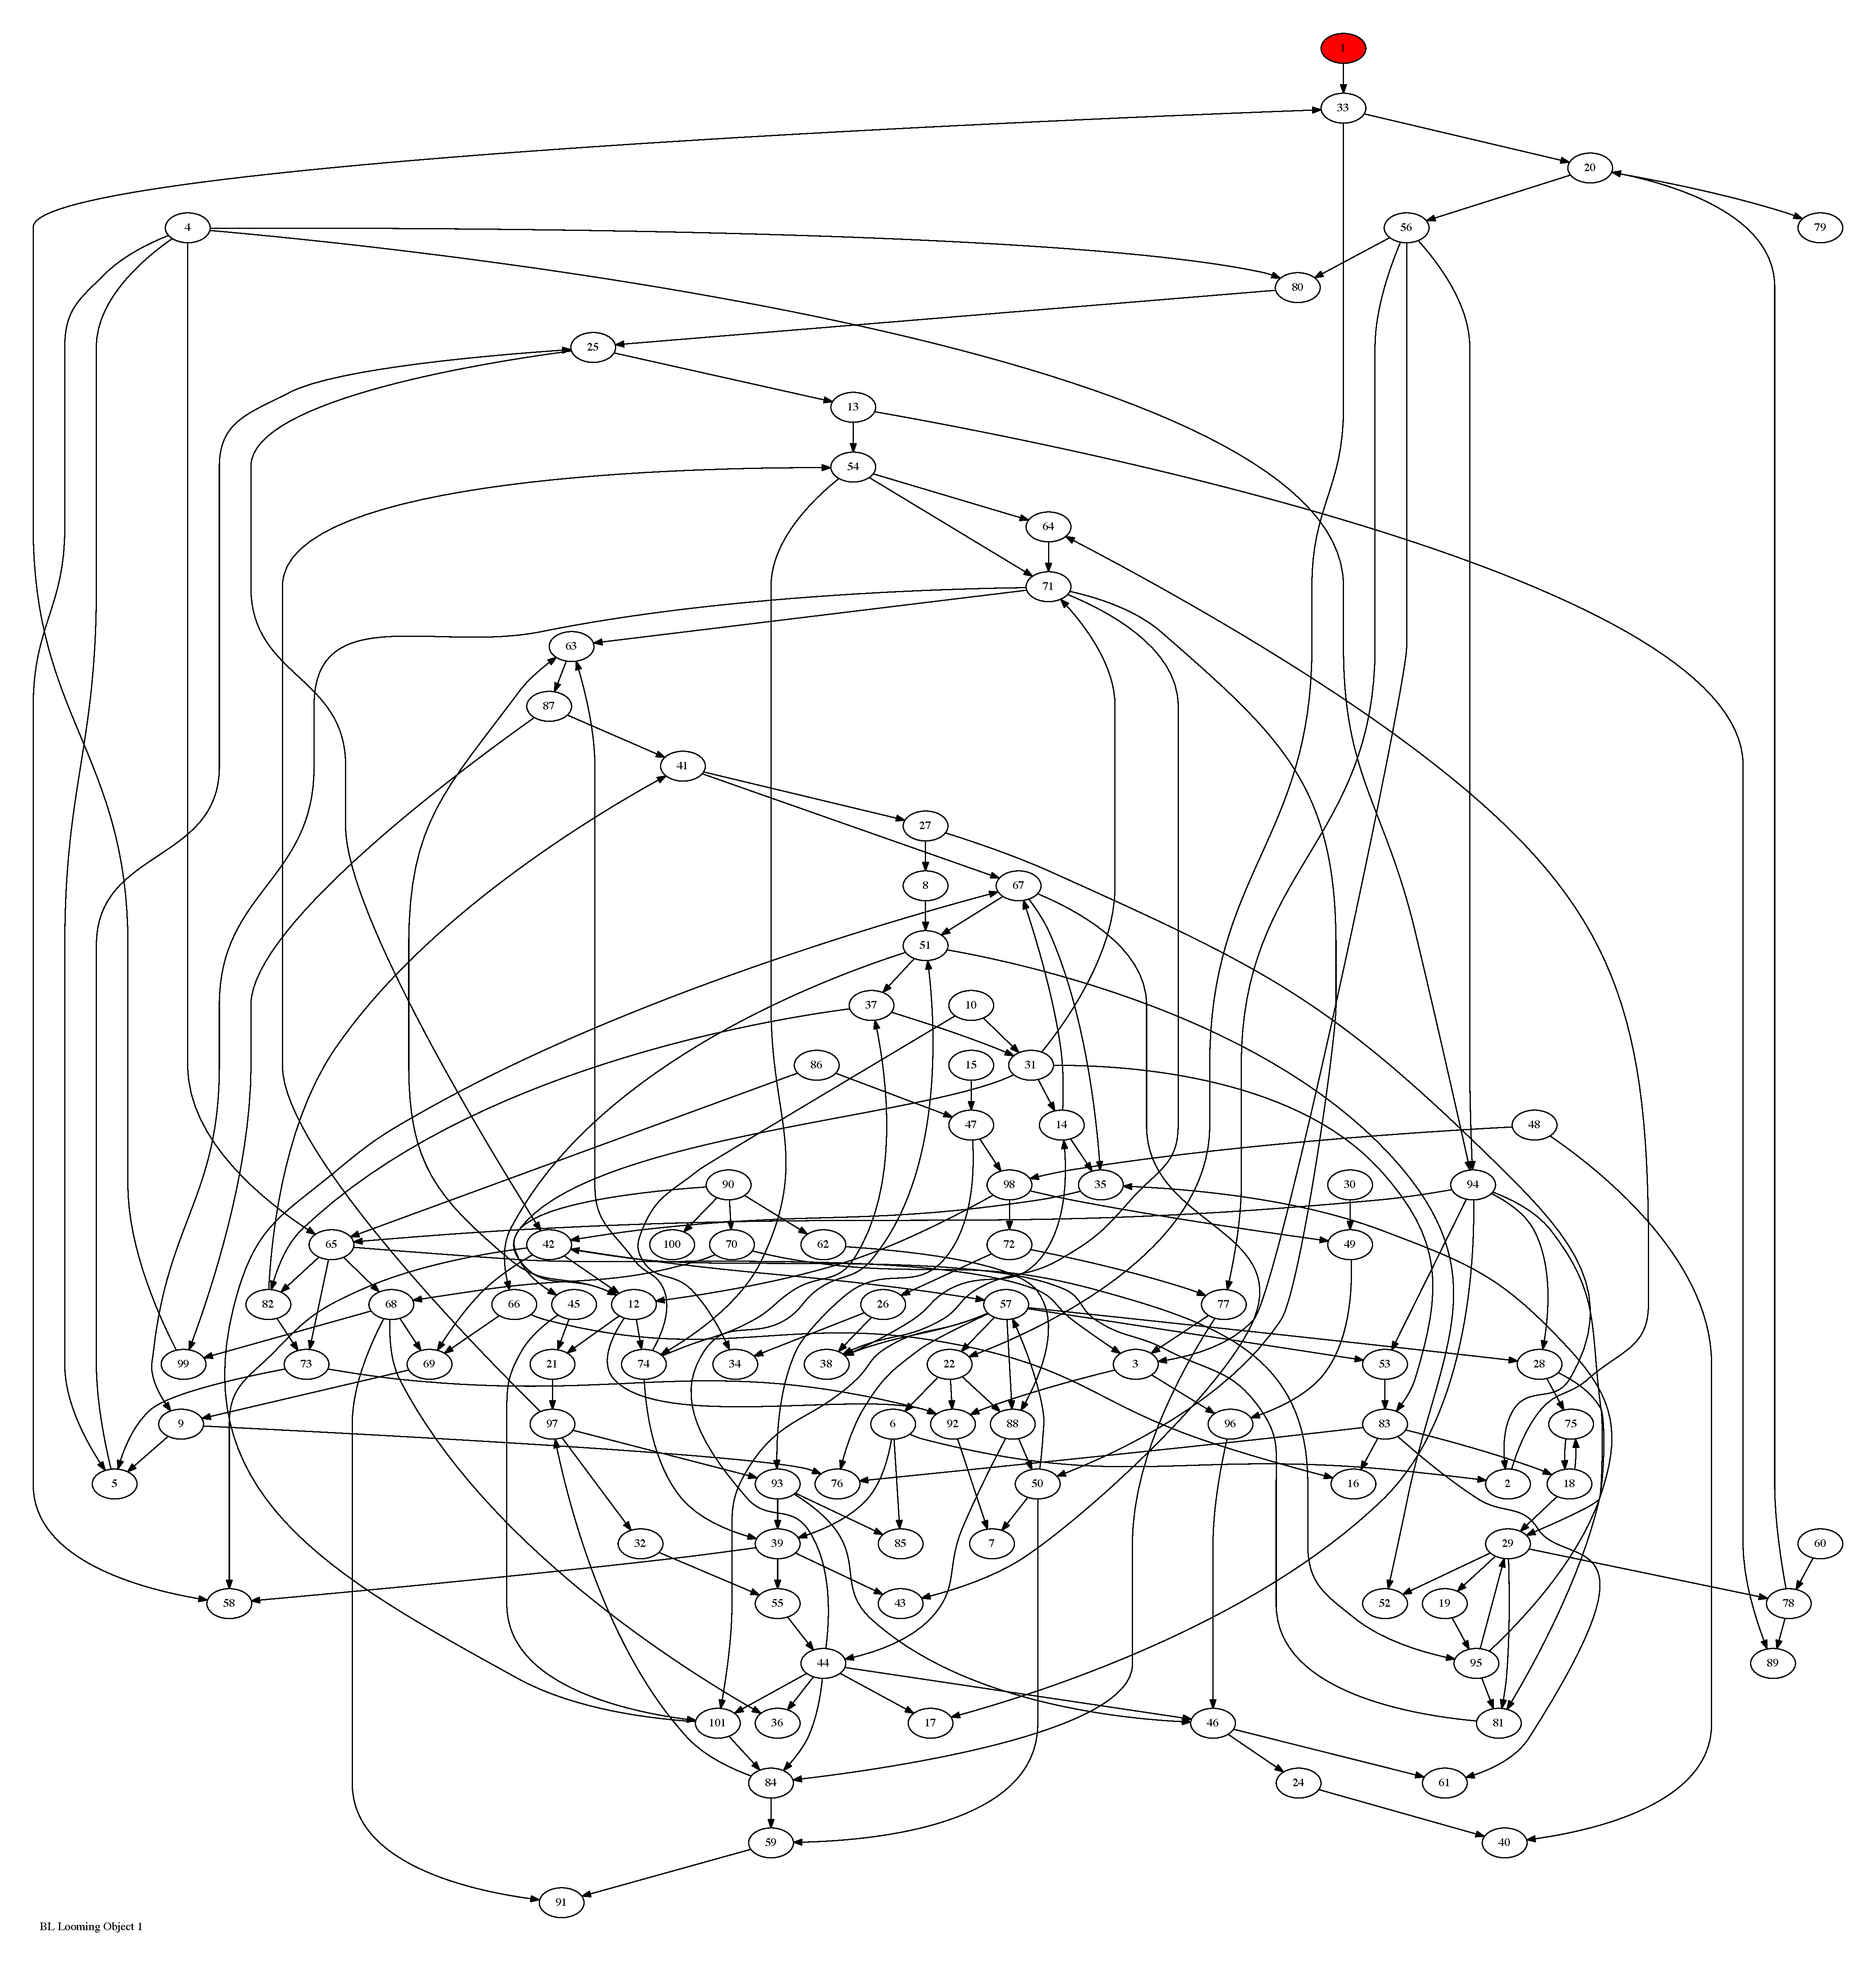
\includegraphics[max height=\textheight,max width=\textwidth]{bl_looming_objs/bl_loom_obj1_pp.pdf}

\newpage
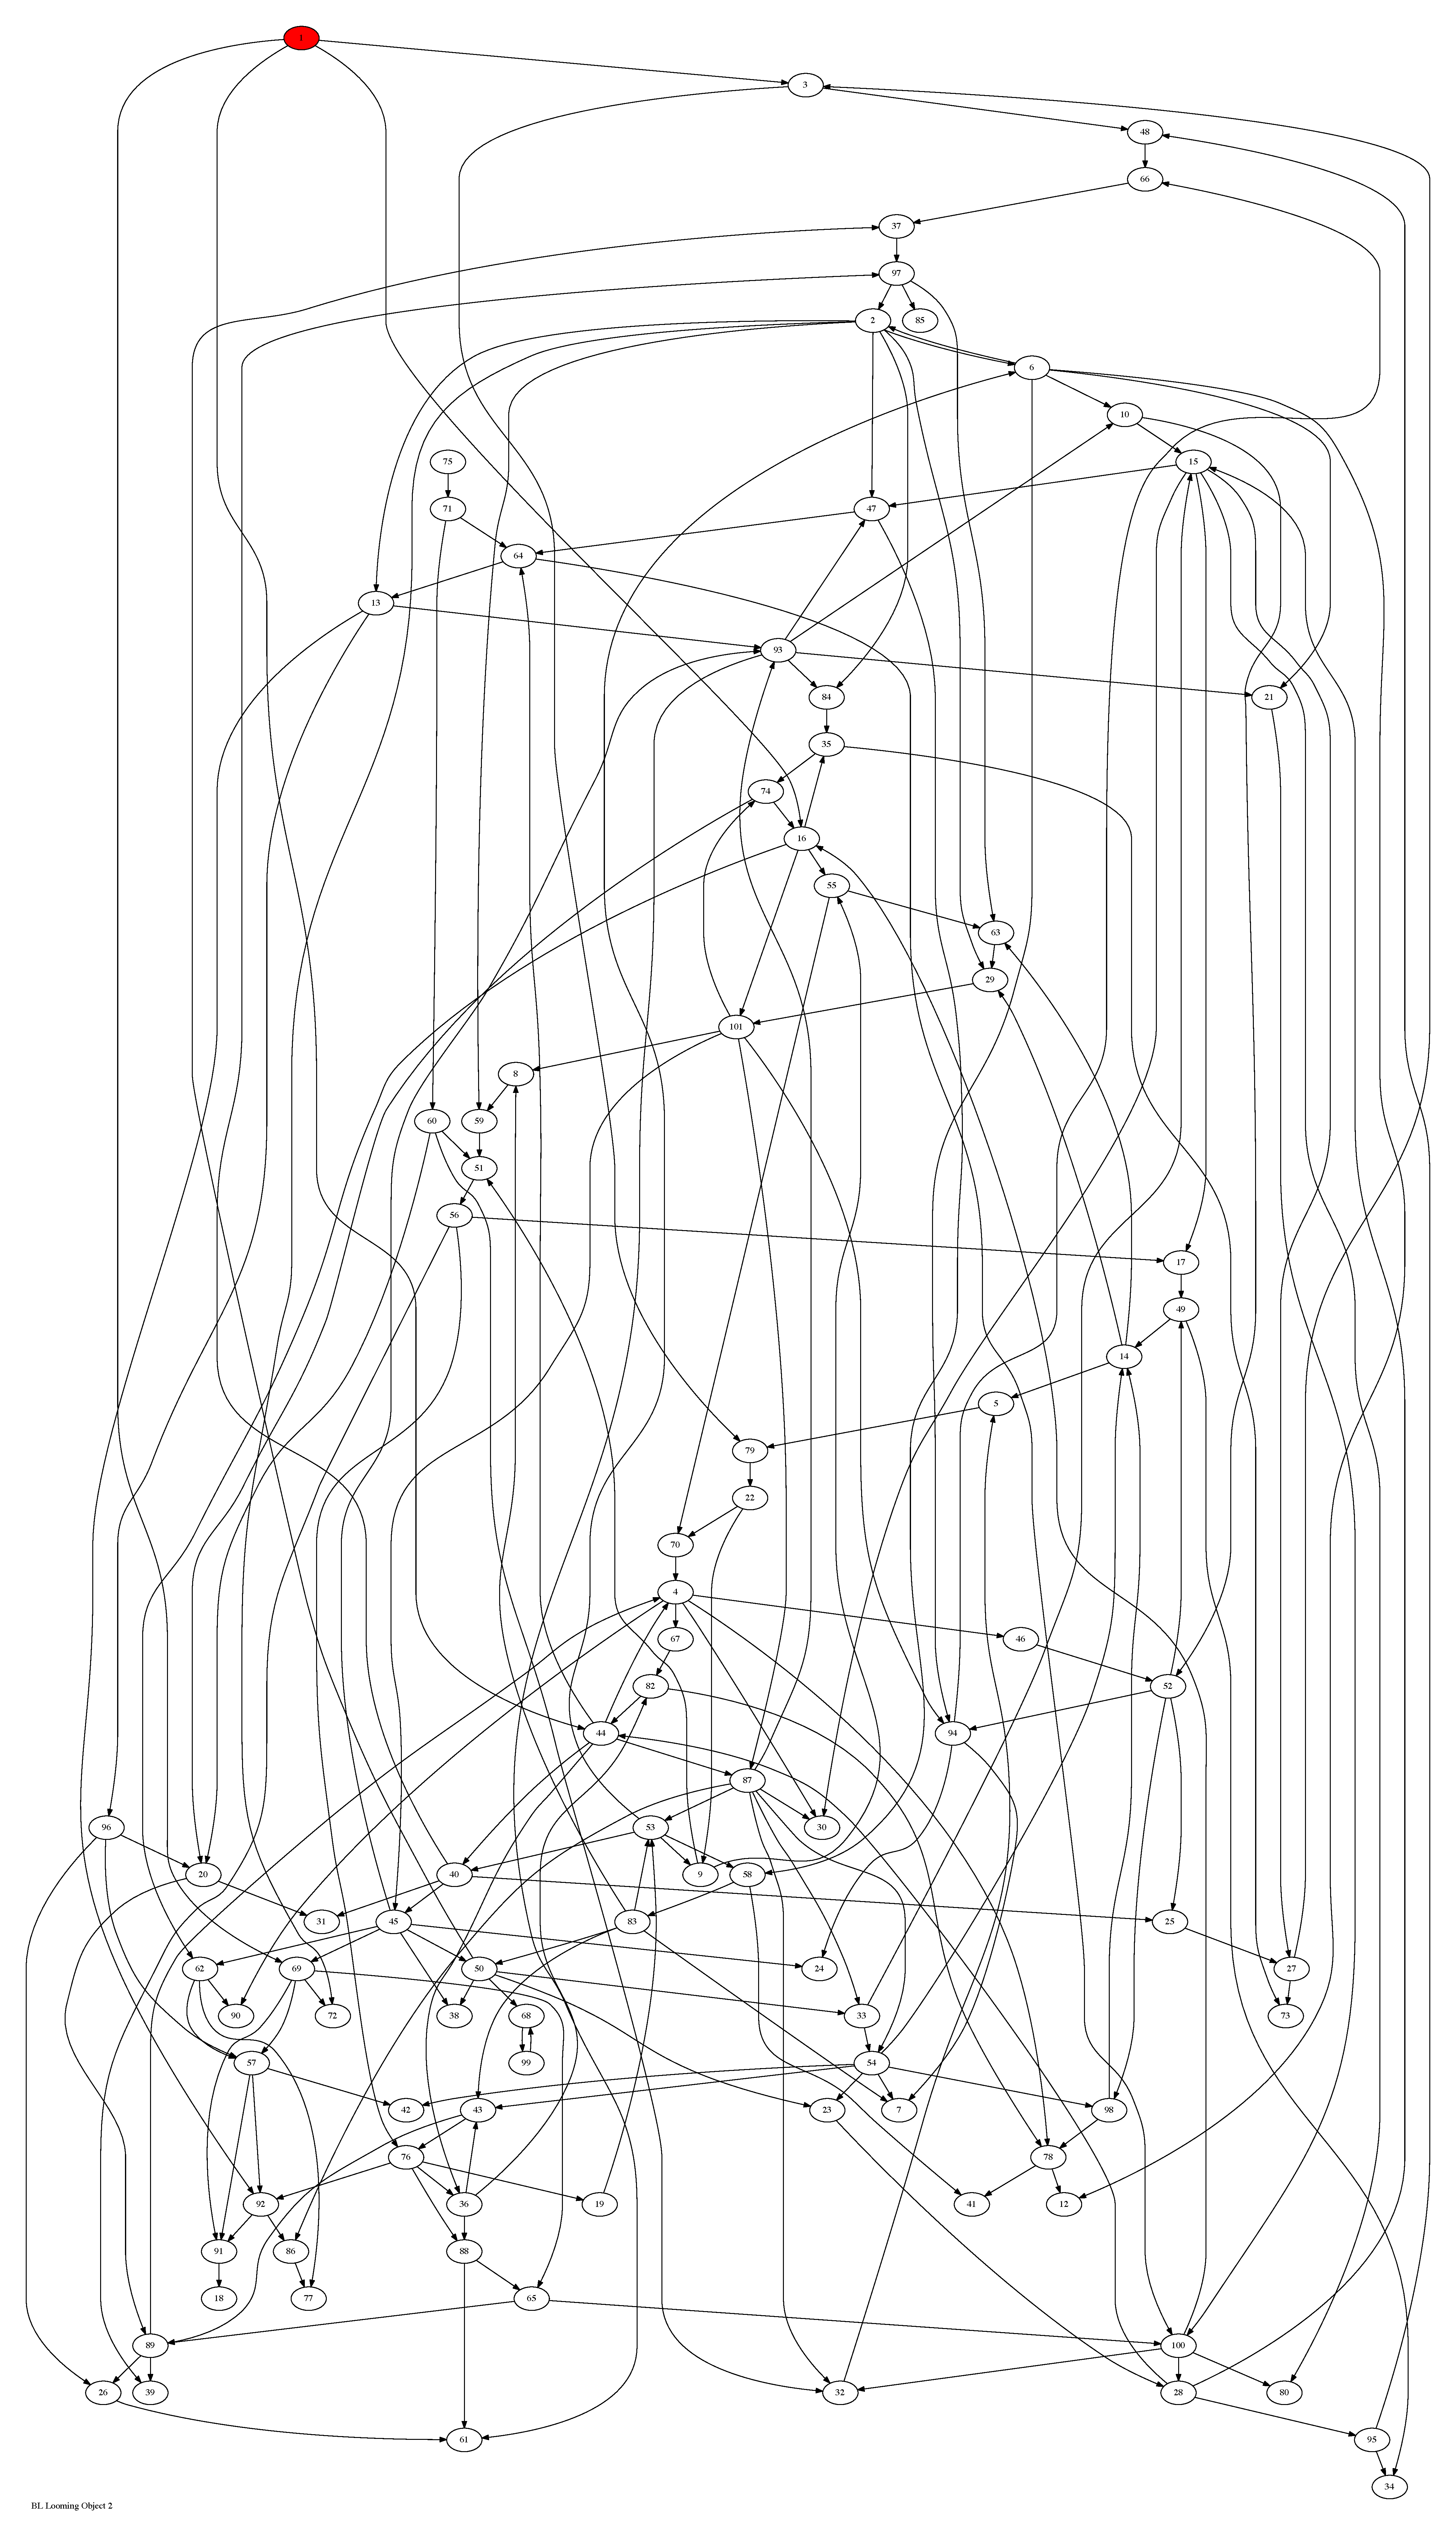
\includegraphics[max height=\textheight,max width=\textwidth]{bl_looming_objs/bl_loom_obj2_pp.pdf}

\newpage
\includegraphics[max height=\textheight,max width=\textwidth]{bl_looming_objs/bl_loom_obj3_pp.pdf}

\newpage
\includegraphics[max height=\textheight,max width=\textwidth]{bl_looming_objs/bl_loom_obj4_pp.pdf}

\newpage
\includegraphics[max height=\textheight,max width=\textwidth]{bl_looming_objs/bl_loom_obj5_pp.pdf}

\newpage
\includegraphics[max height=\textheight,max width=\textwidth]{bl_looming_objs/bl_loom_obj6_pp.pdf}

\newpage
\includegraphics[max height=\textheight,max width=\textwidth]{bl_looming_objs/bl_loom_obj7_pp.pdf}

\newpage
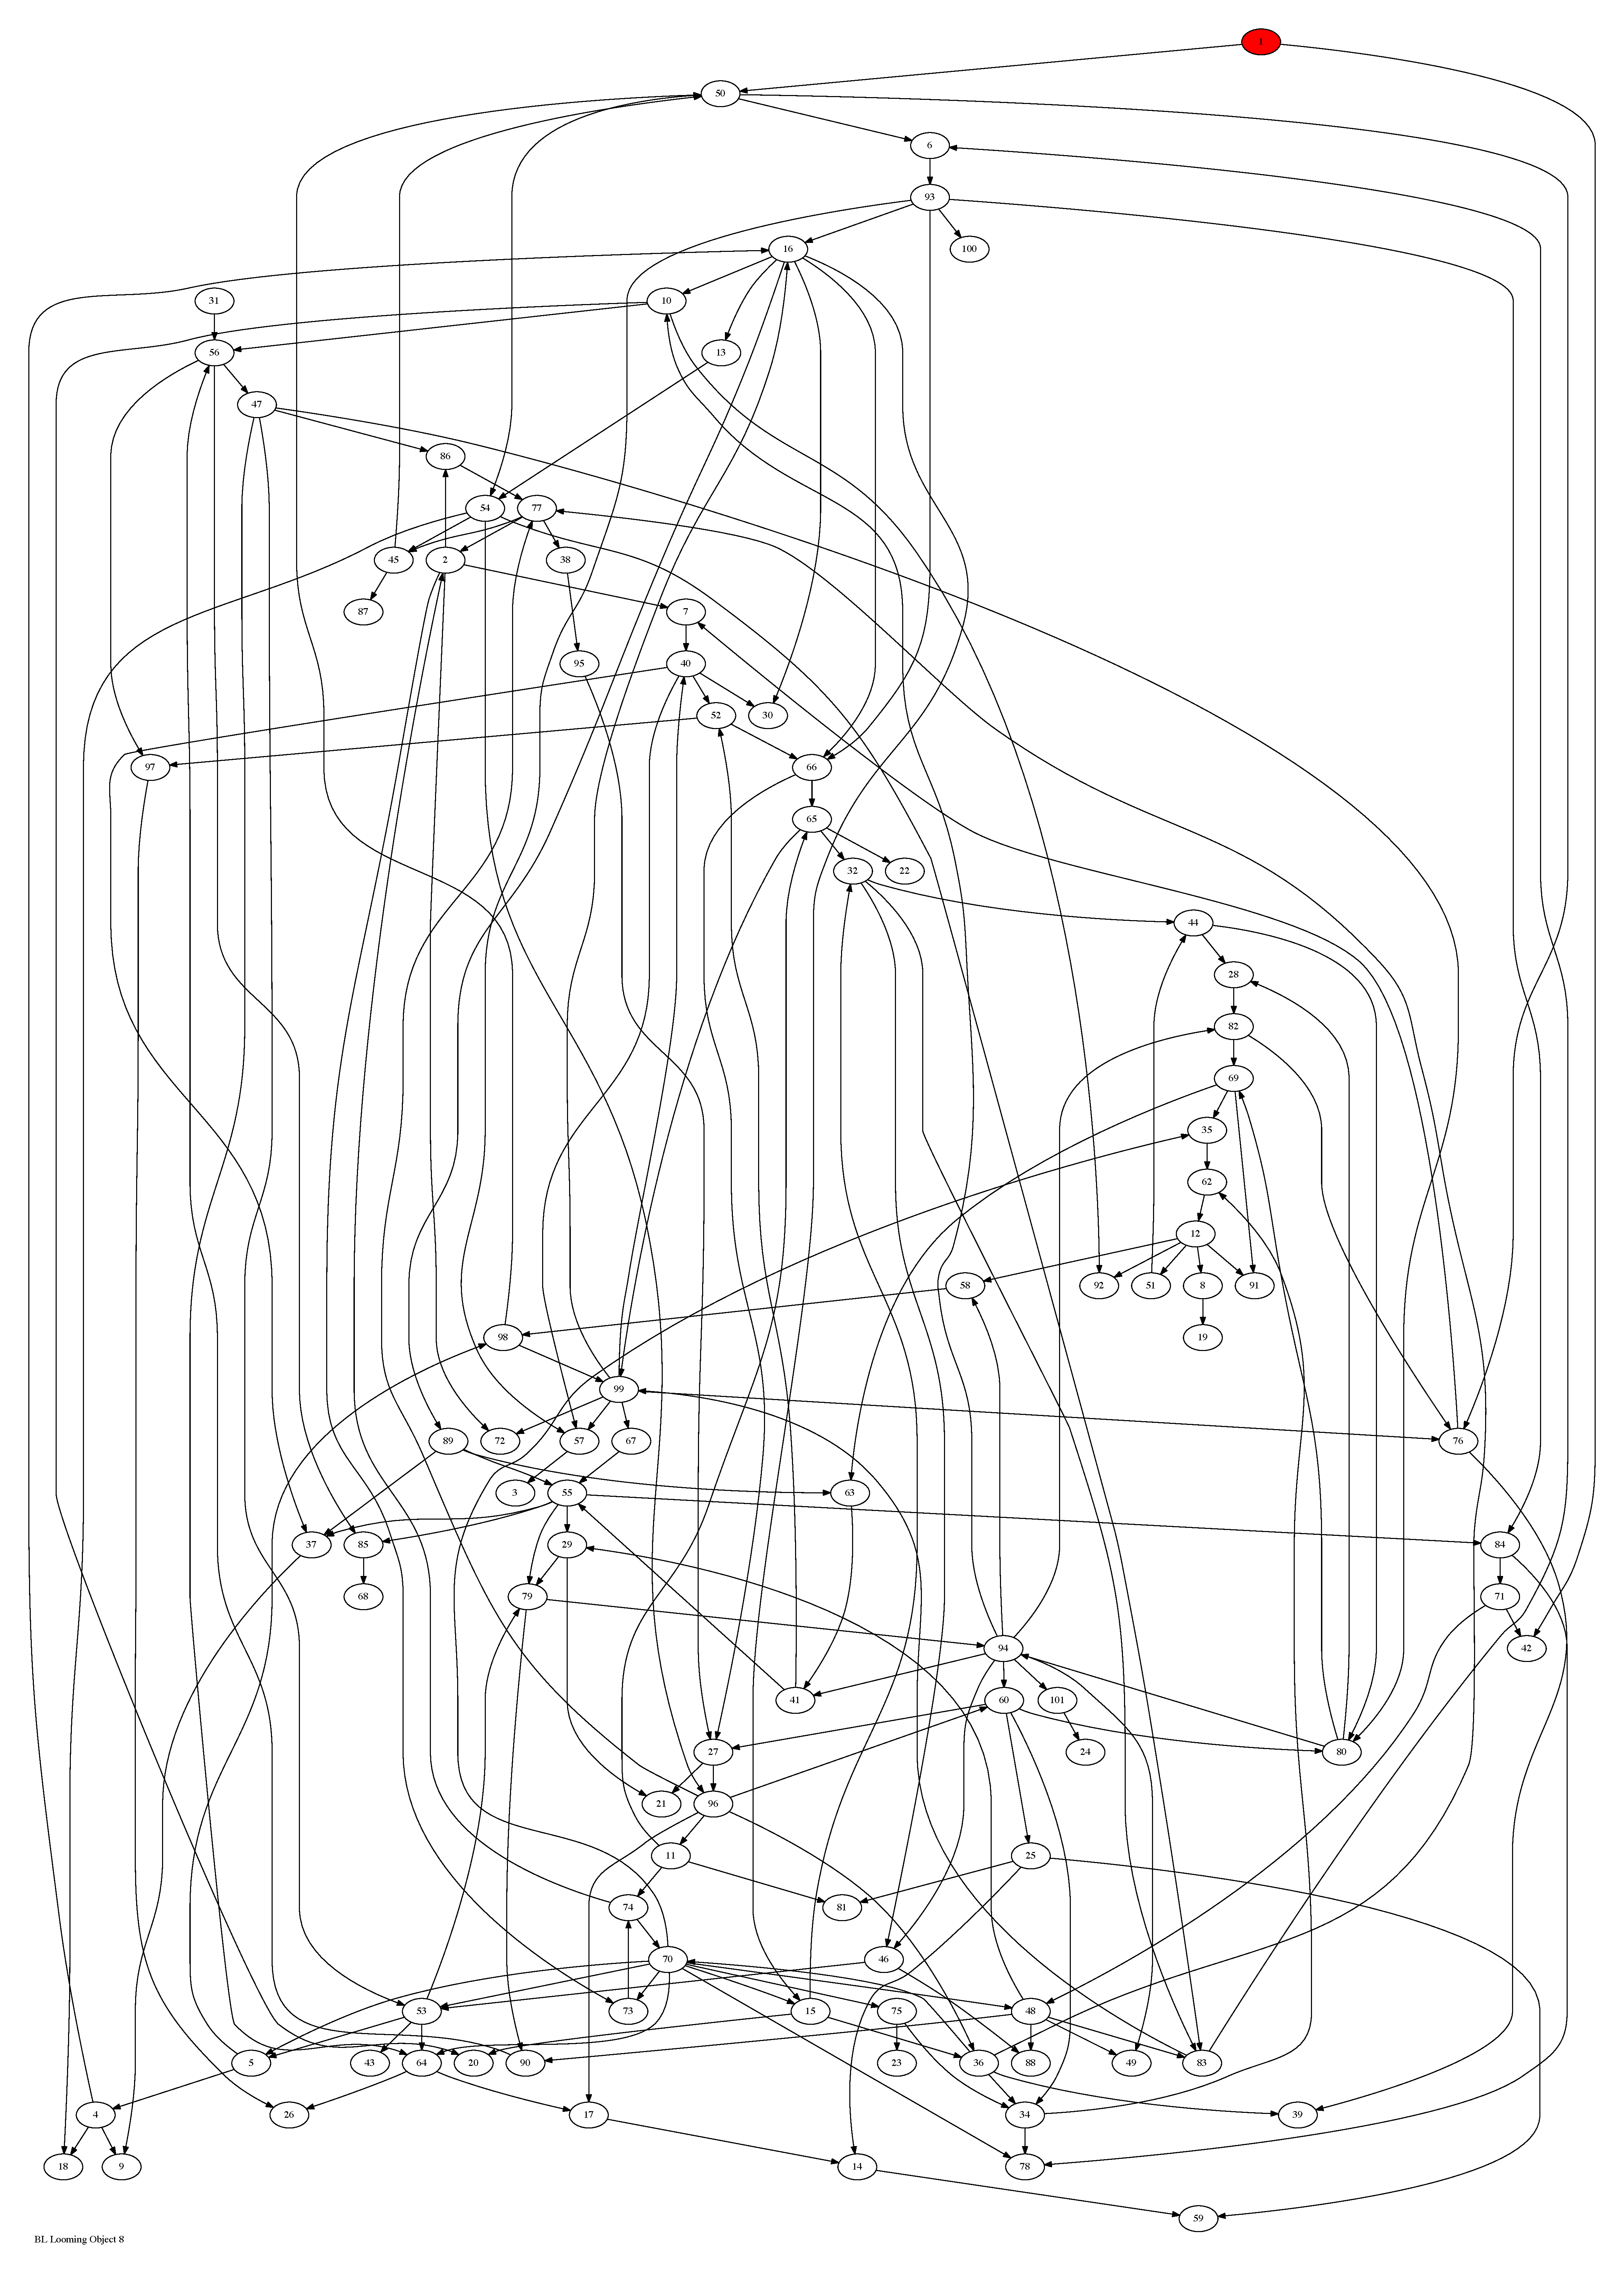
\includegraphics[max height=\textheight,max width=\textwidth]{bl_looming_objs/bl_loom_obj8_pp.pdf}

\newpage
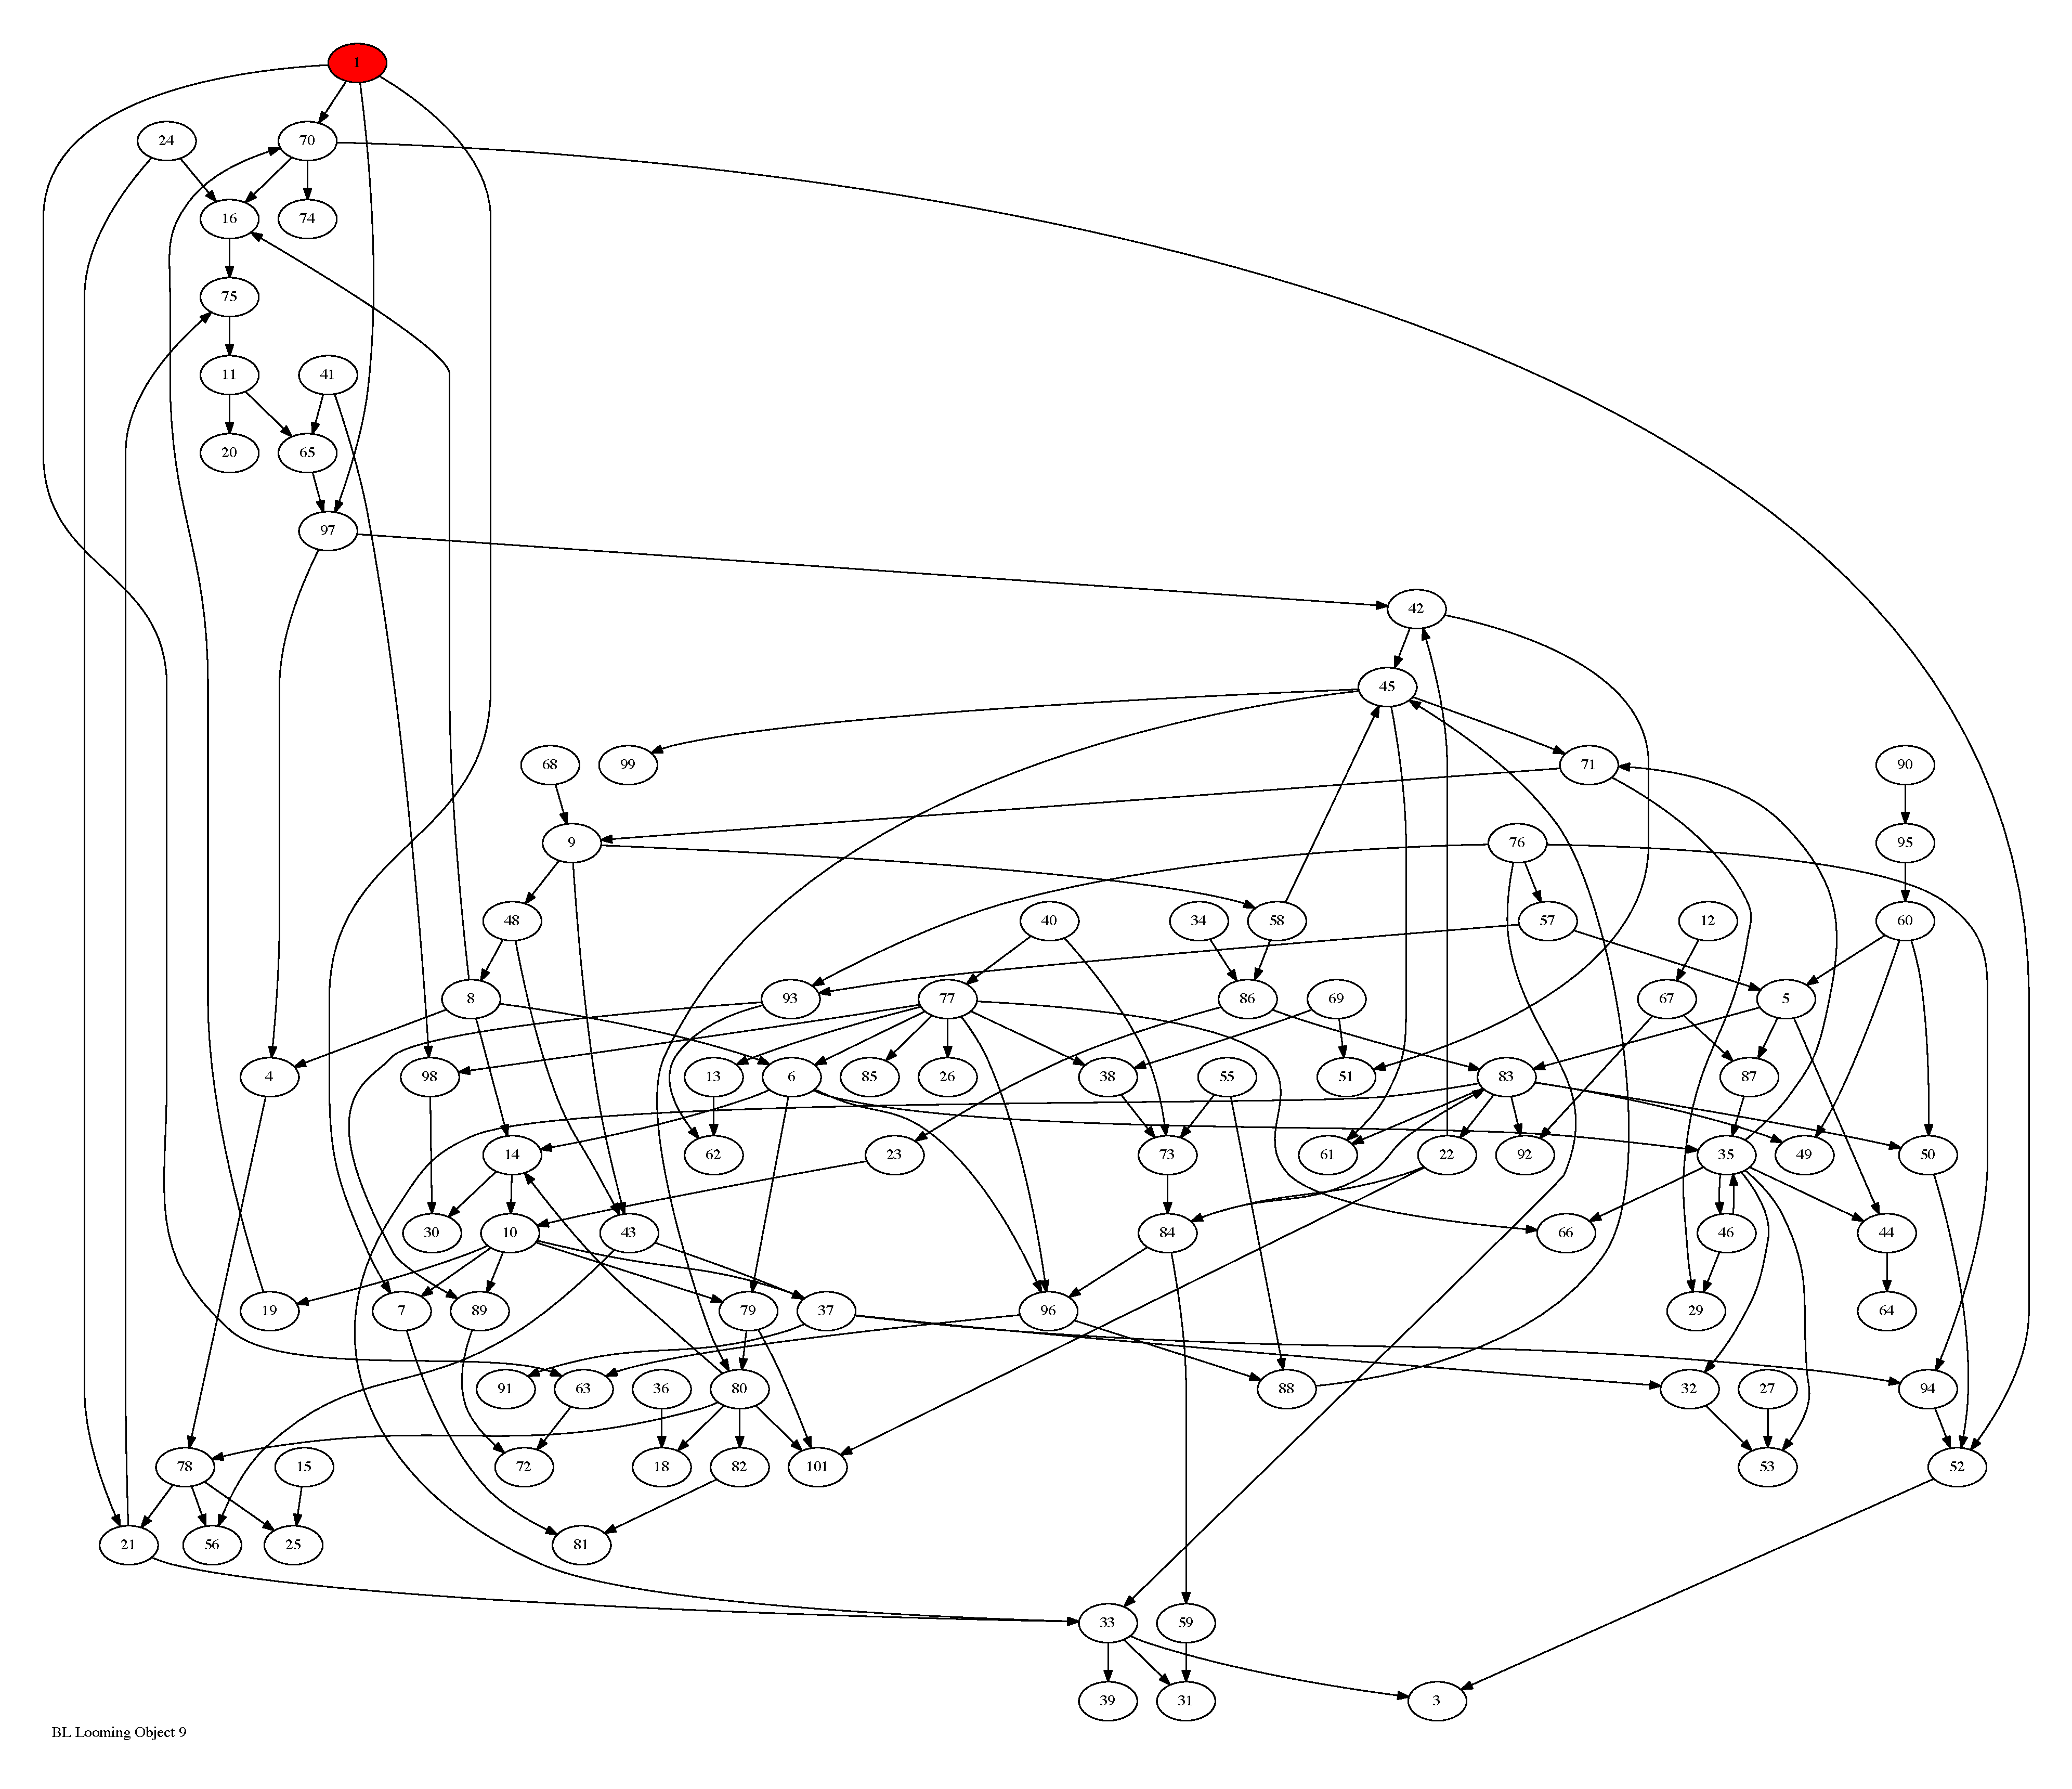
\includegraphics[max height=\textheight,max width=\textwidth]{bl_looming_objs/bl_loom_obj9_pp.pdf}

\newpage
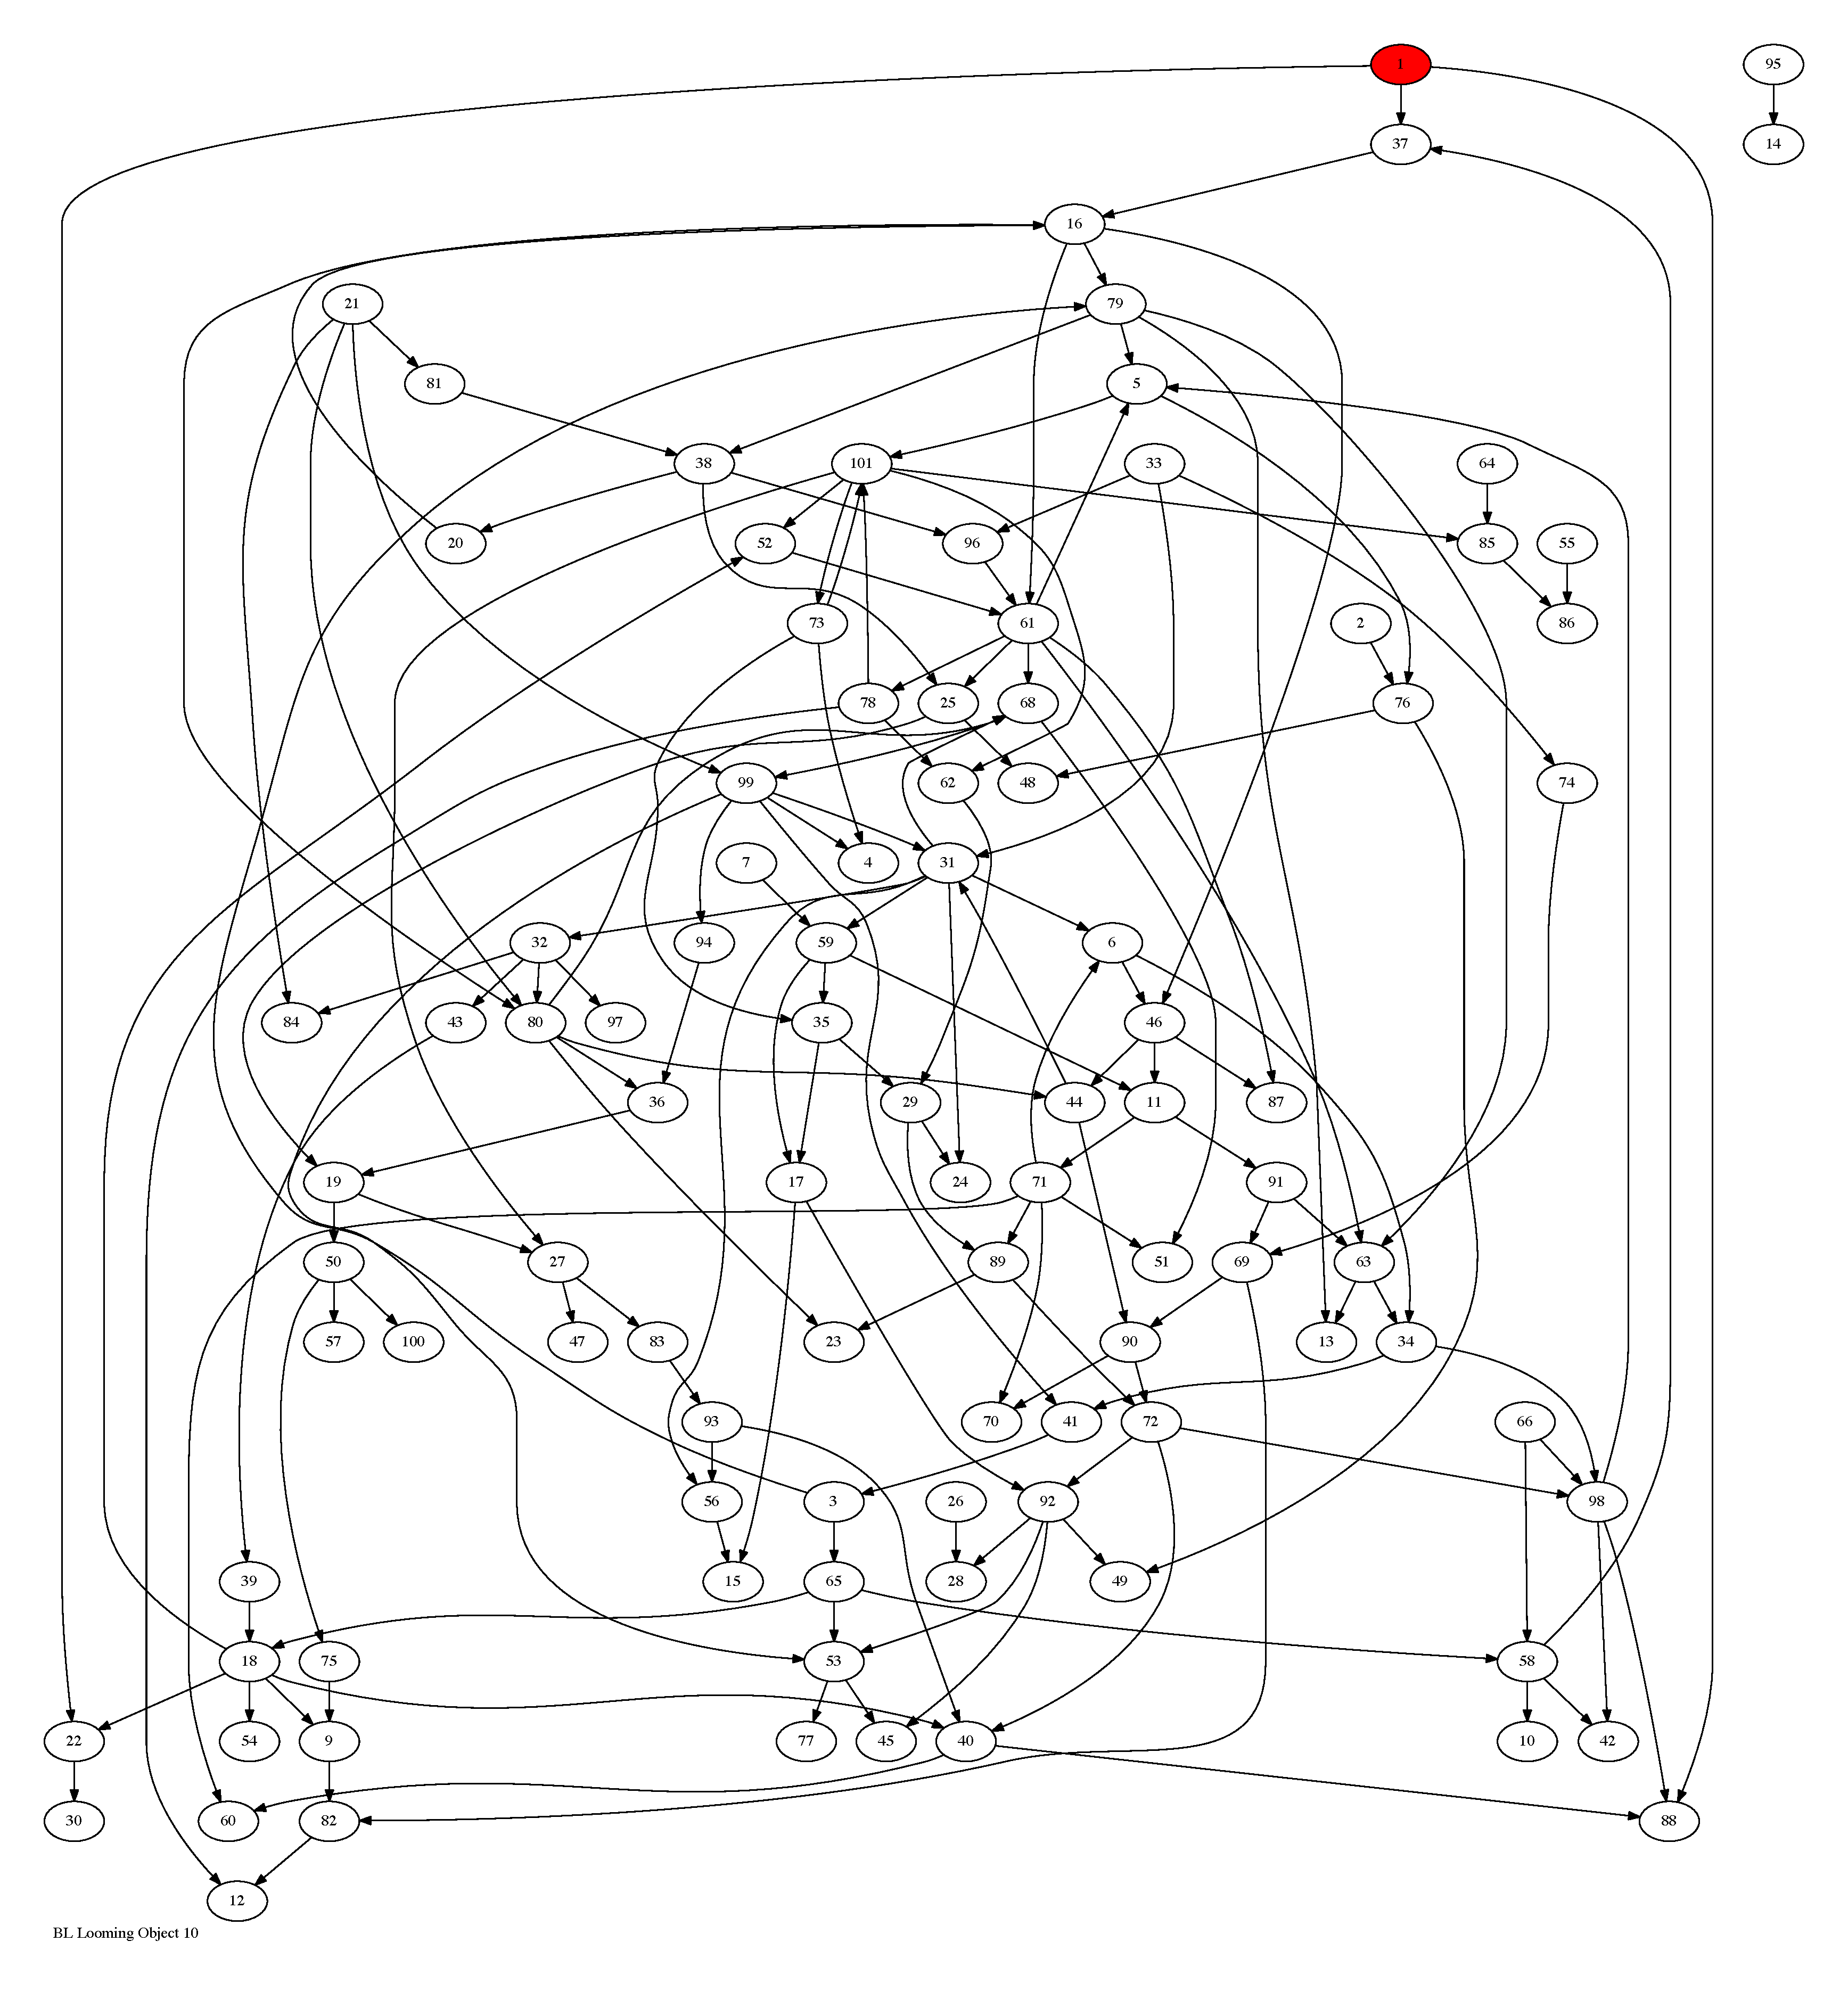
\includegraphics[max height=\textheight,max width=\textwidth]{bl_looming_objs/bl_loom_obj10_pp.pdf}

\newpage
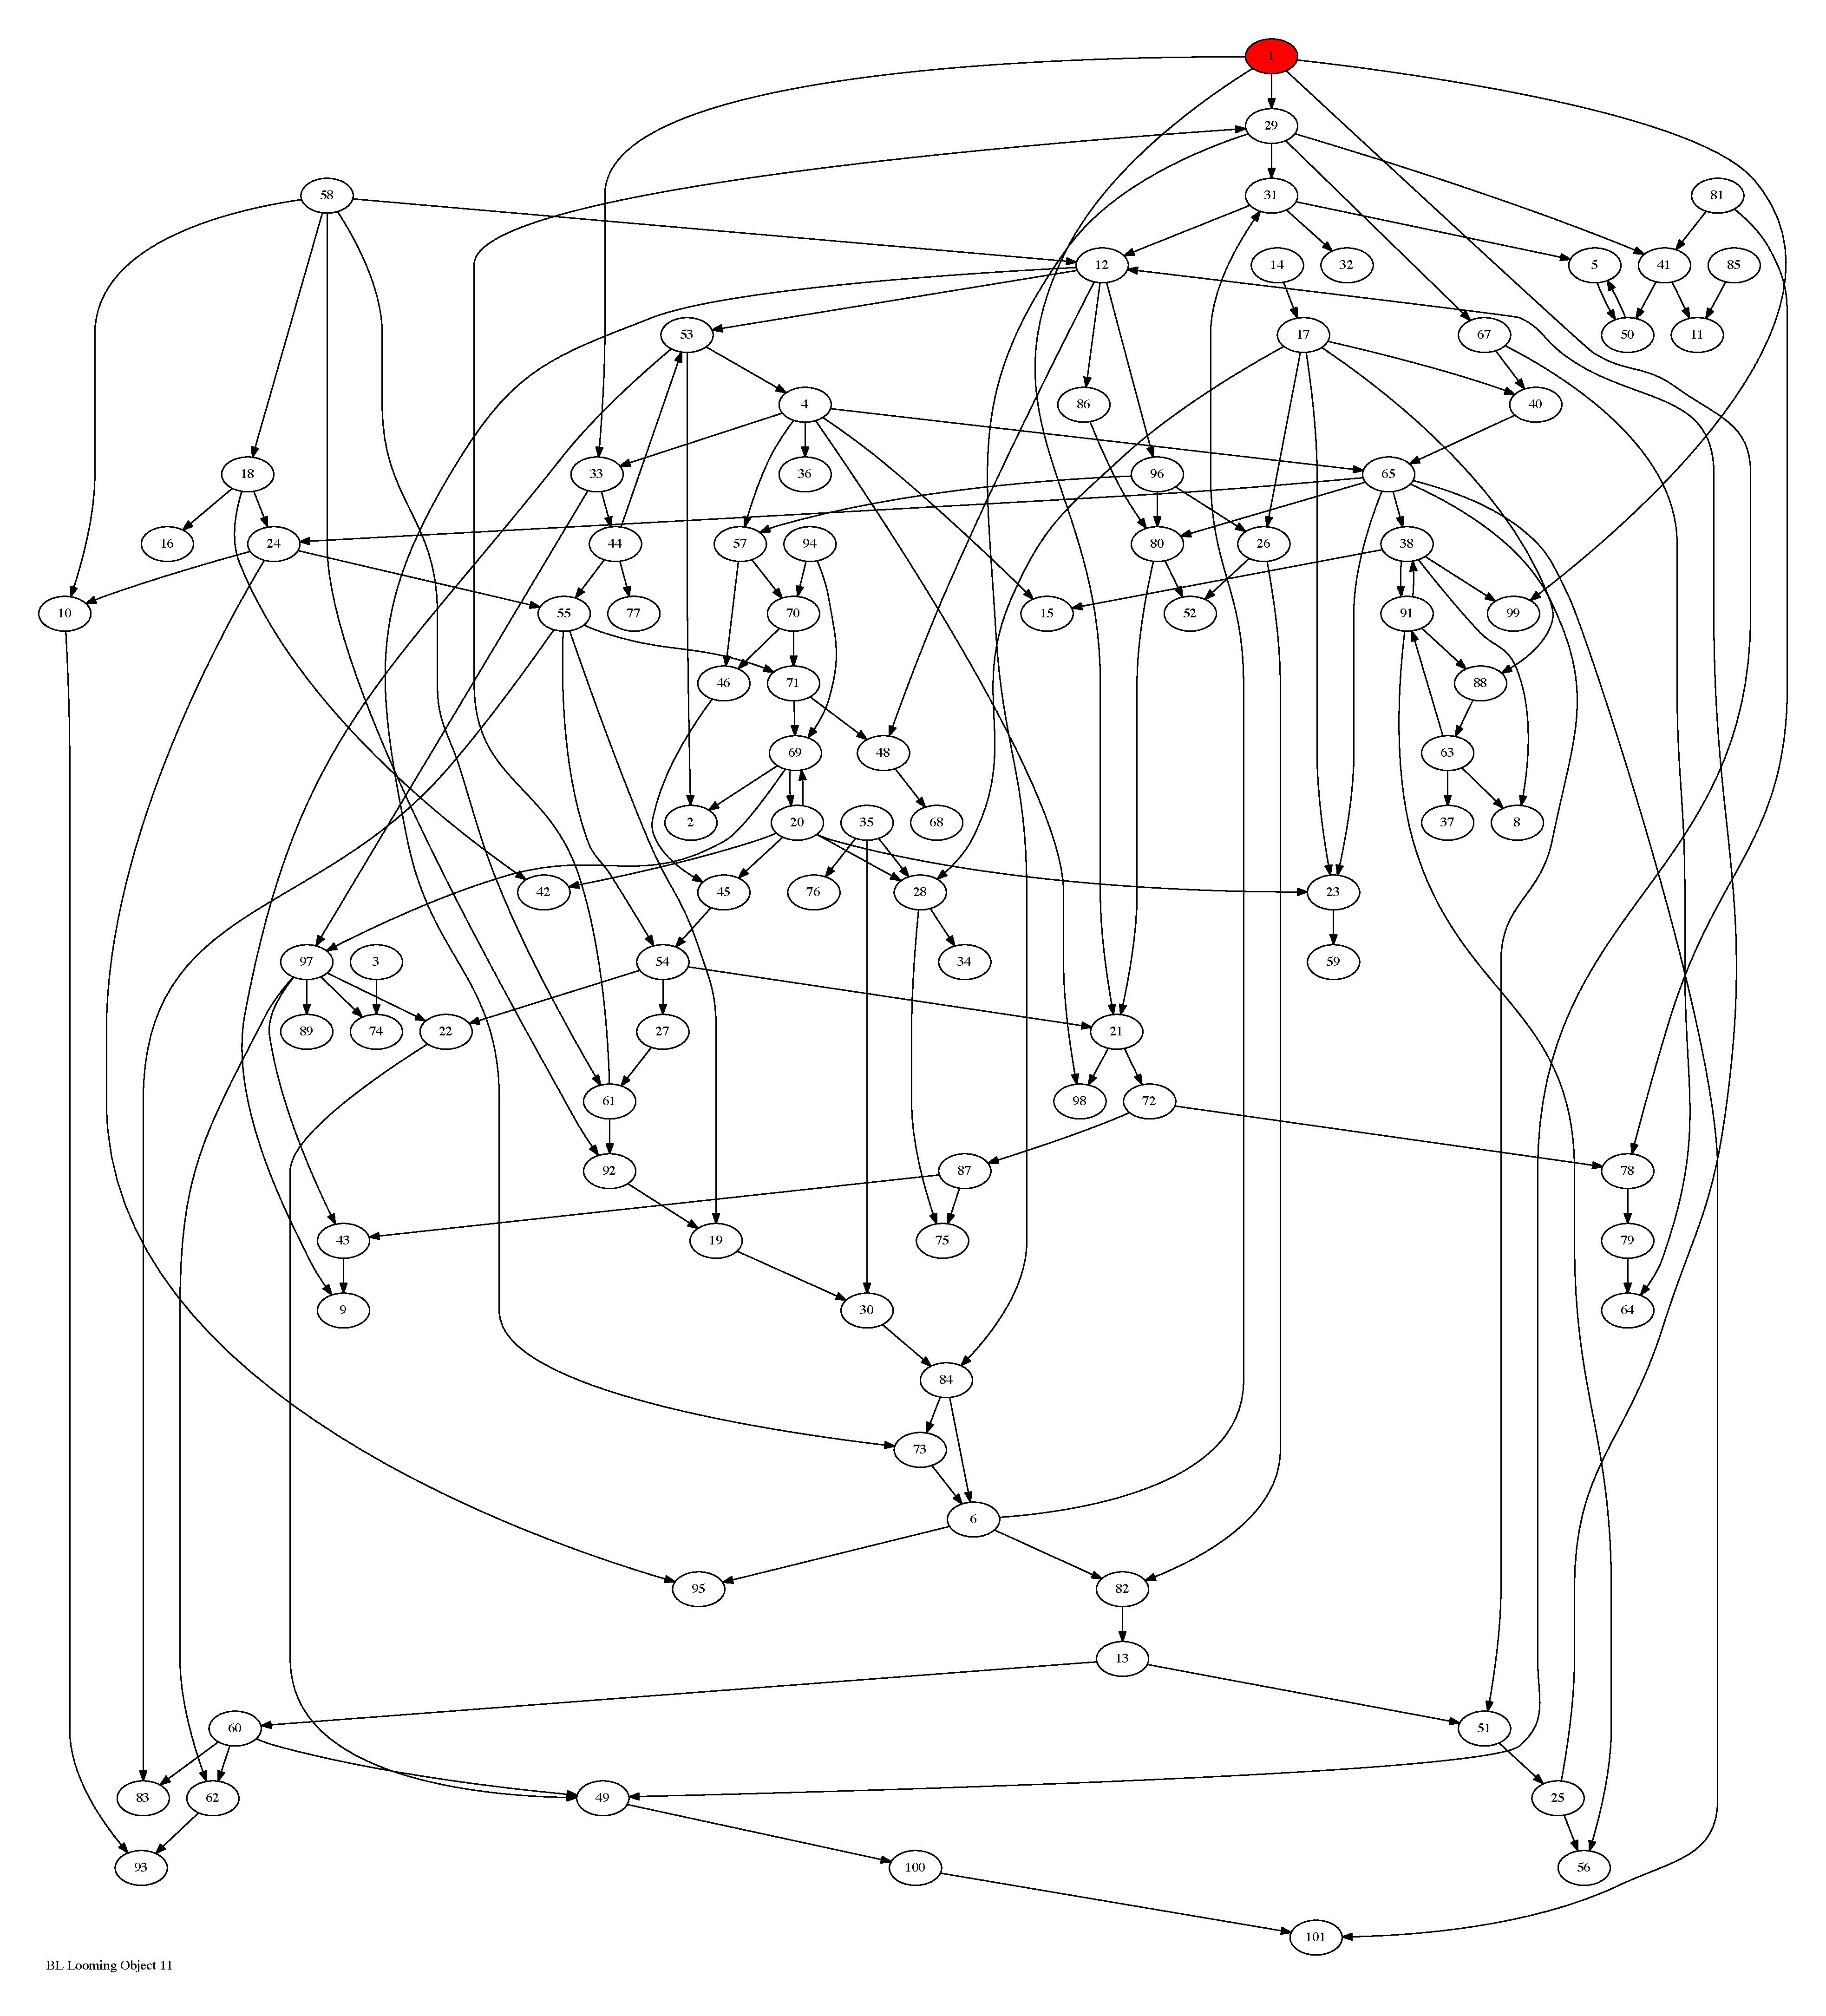
\includegraphics[max height=\textheight,max width=\textwidth]{bl_looming_objs/bl_loom_obj11_pp.pdf}

\newpage
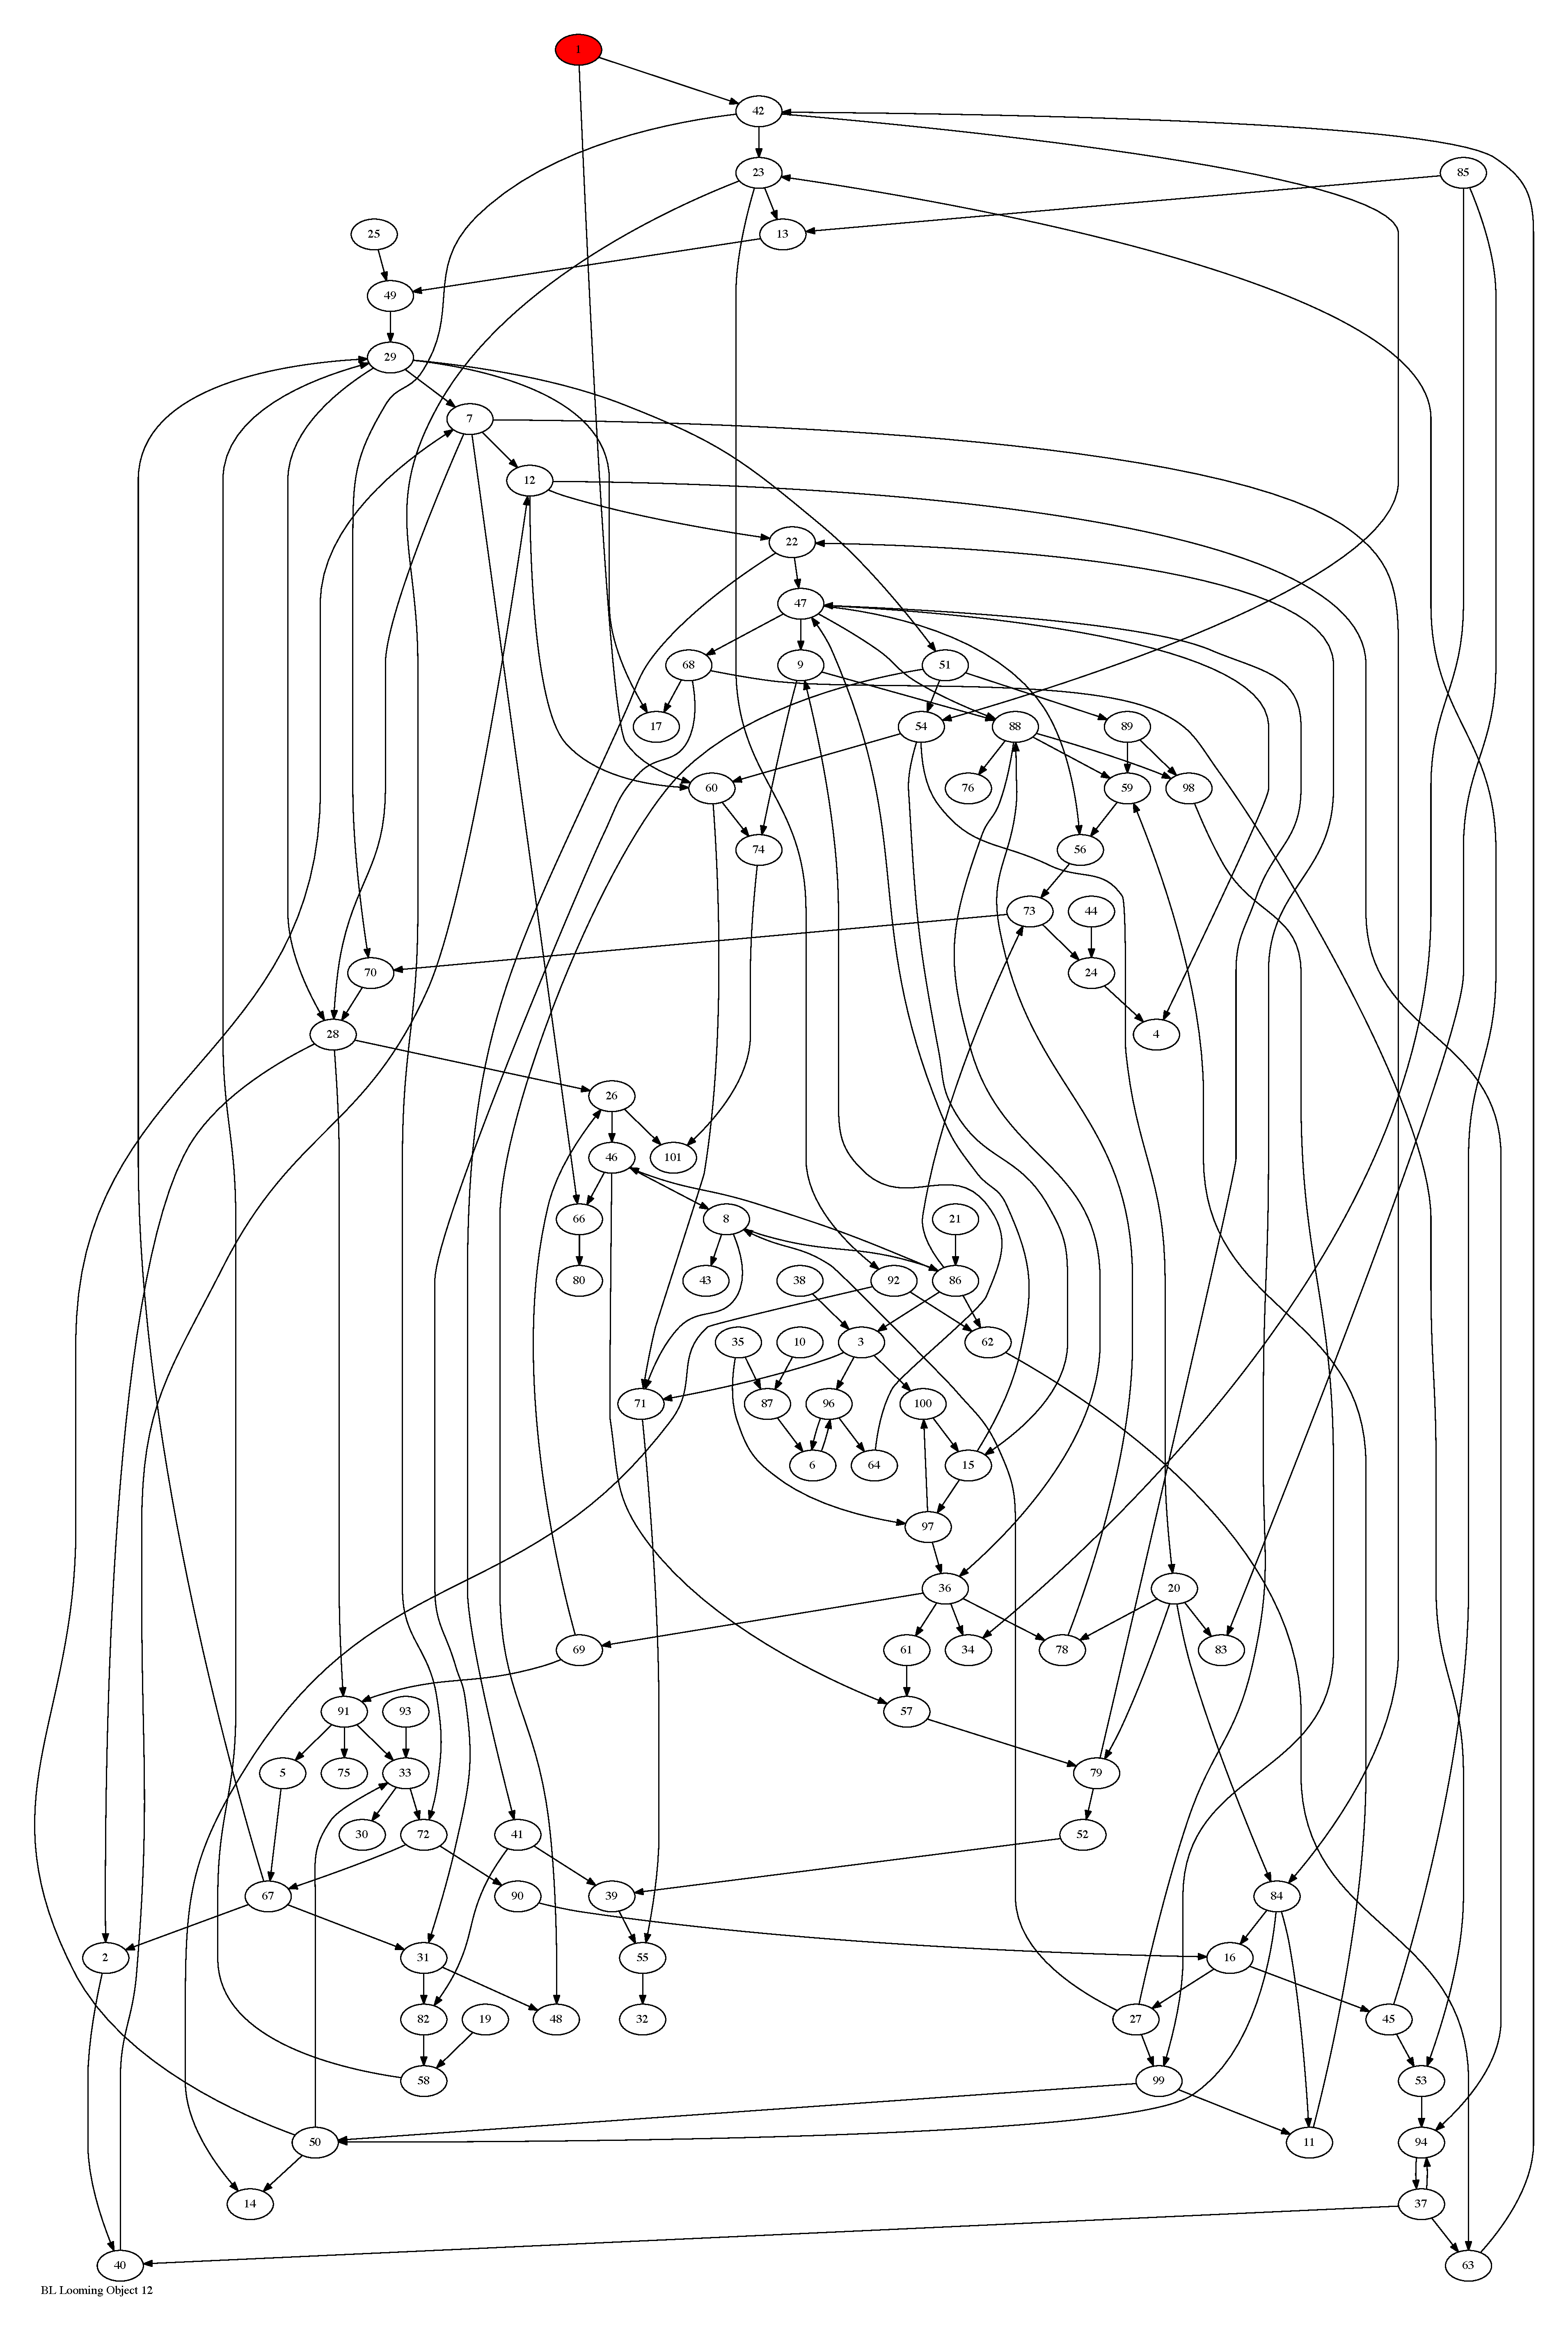
\includegraphics[max height=\textheight,max width=\textwidth]{bl_looming_objs/bl_loom_obj12_pp.pdf}

\newpage
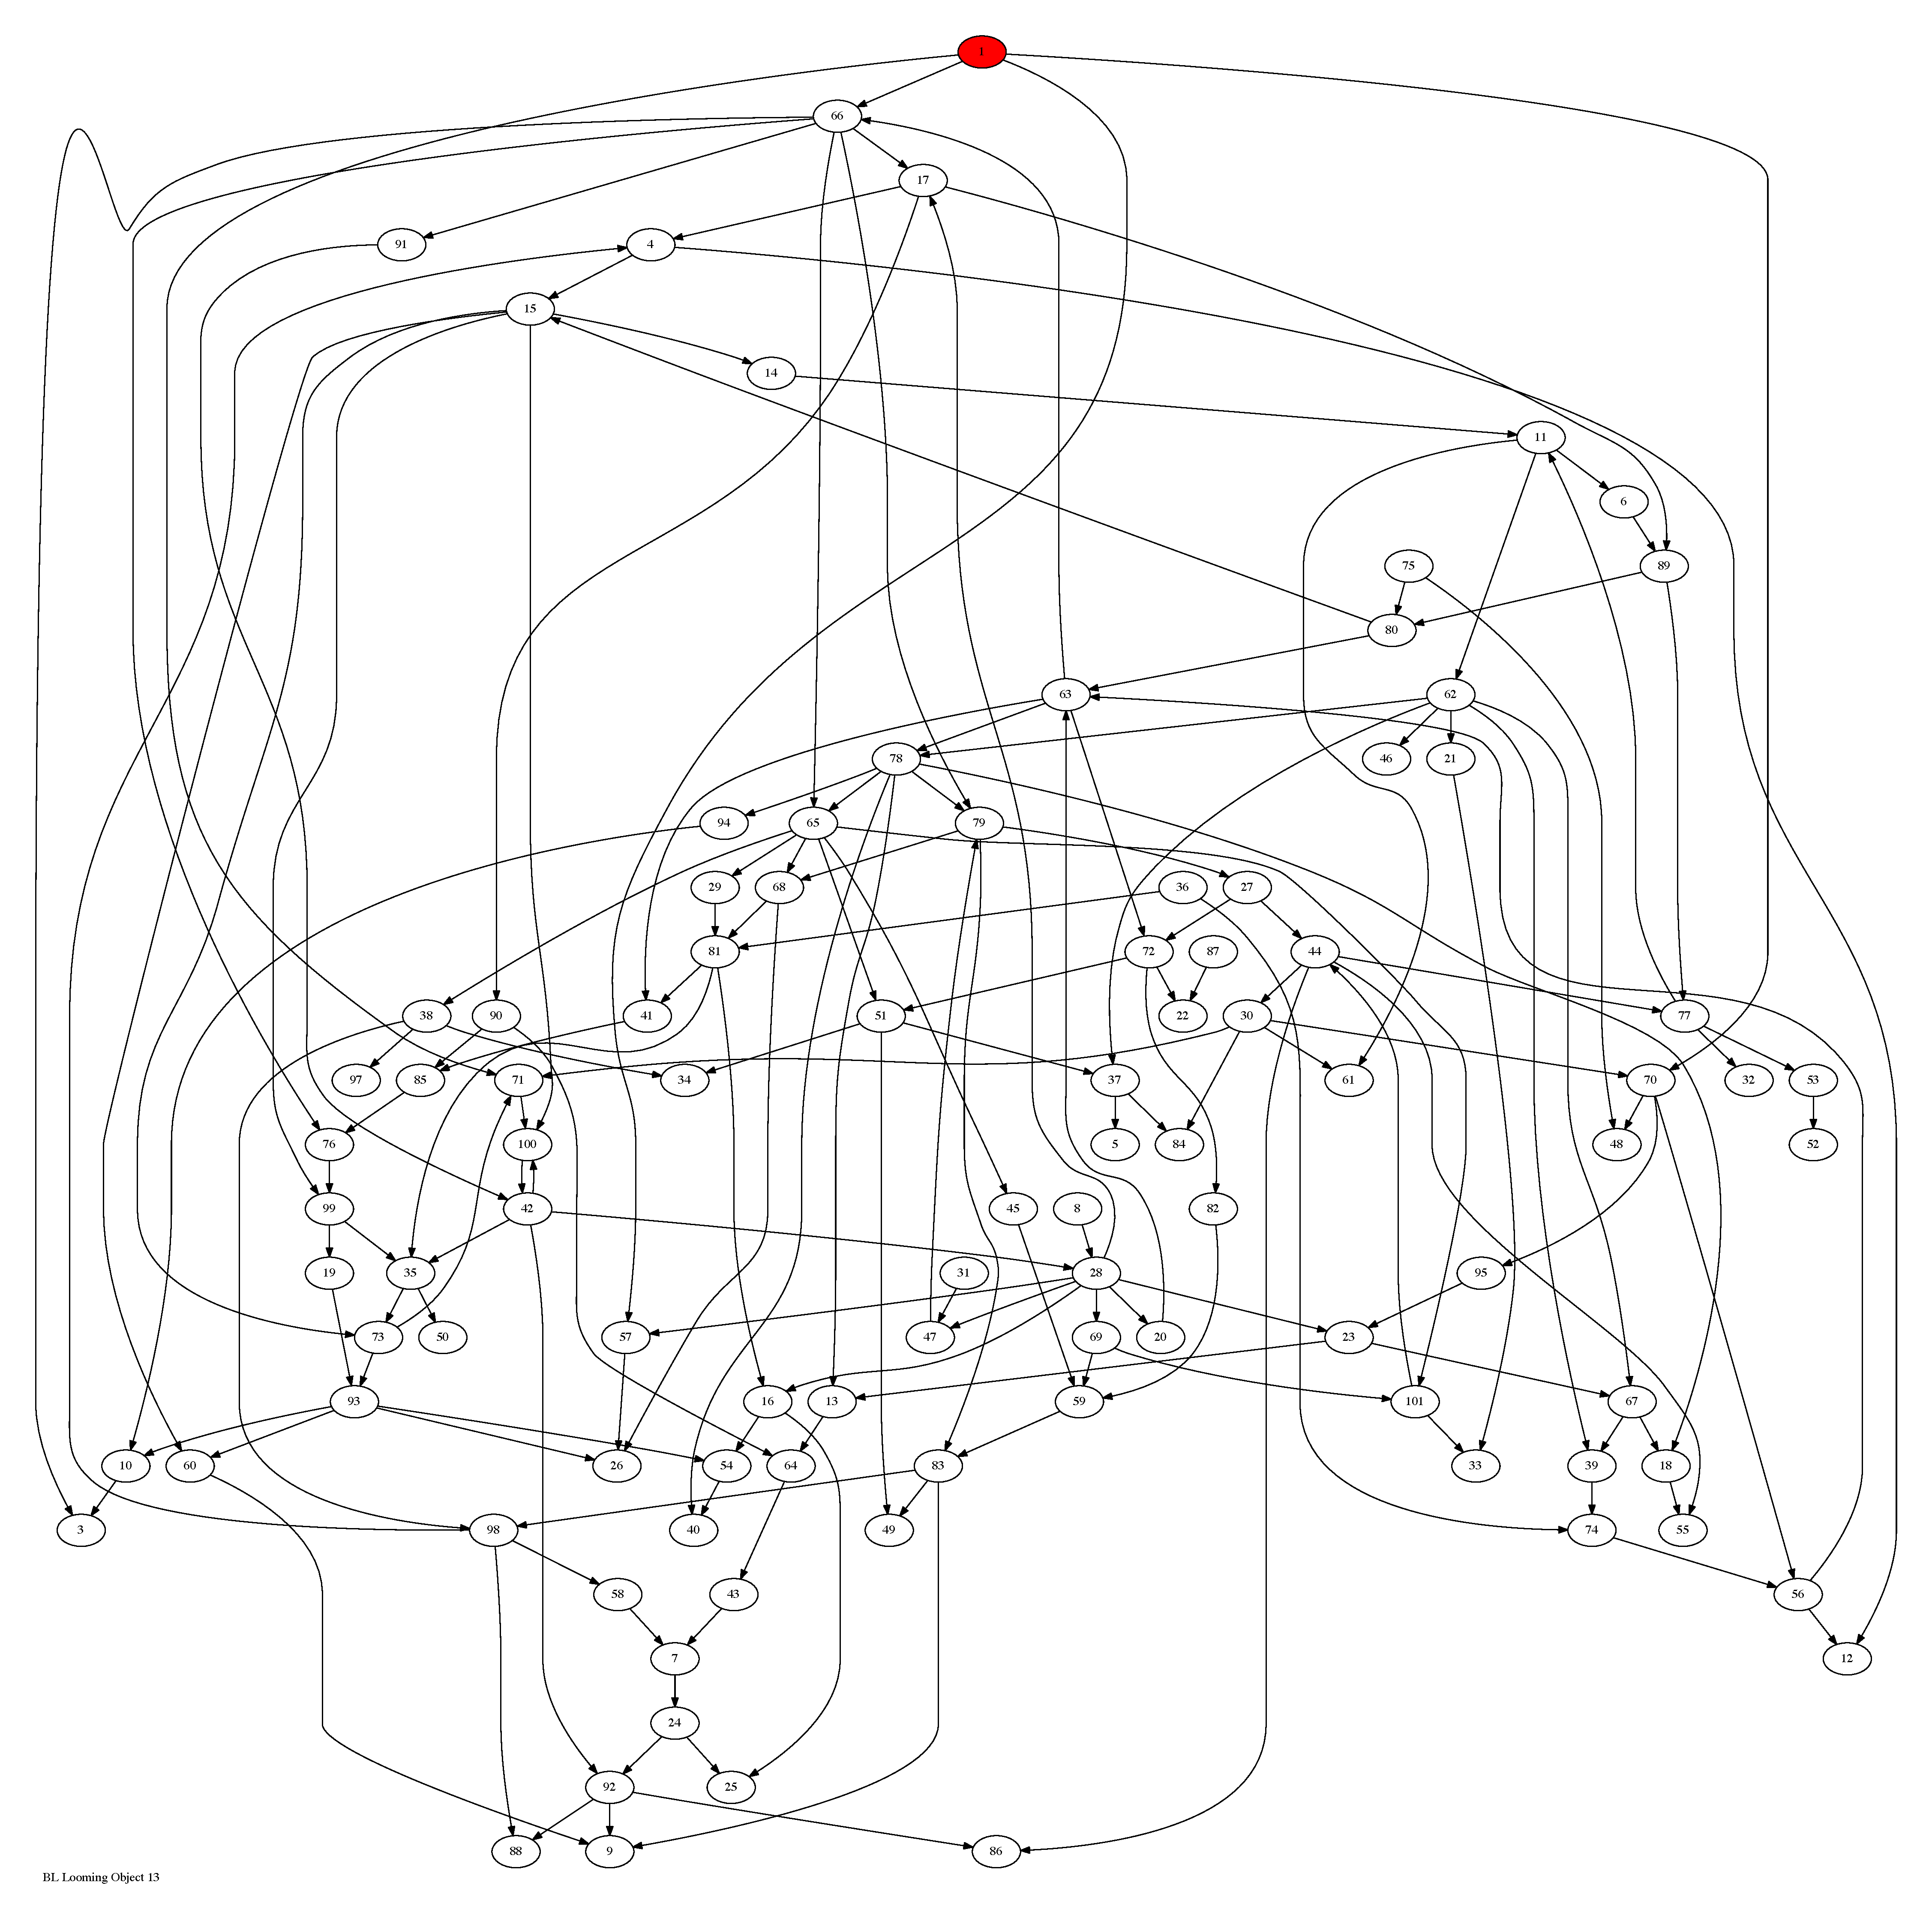
\includegraphics[max height=\textheight,max width=\textwidth]{bl_looming_objs/bl_loom_obj13_pp.pdf}

\newpage
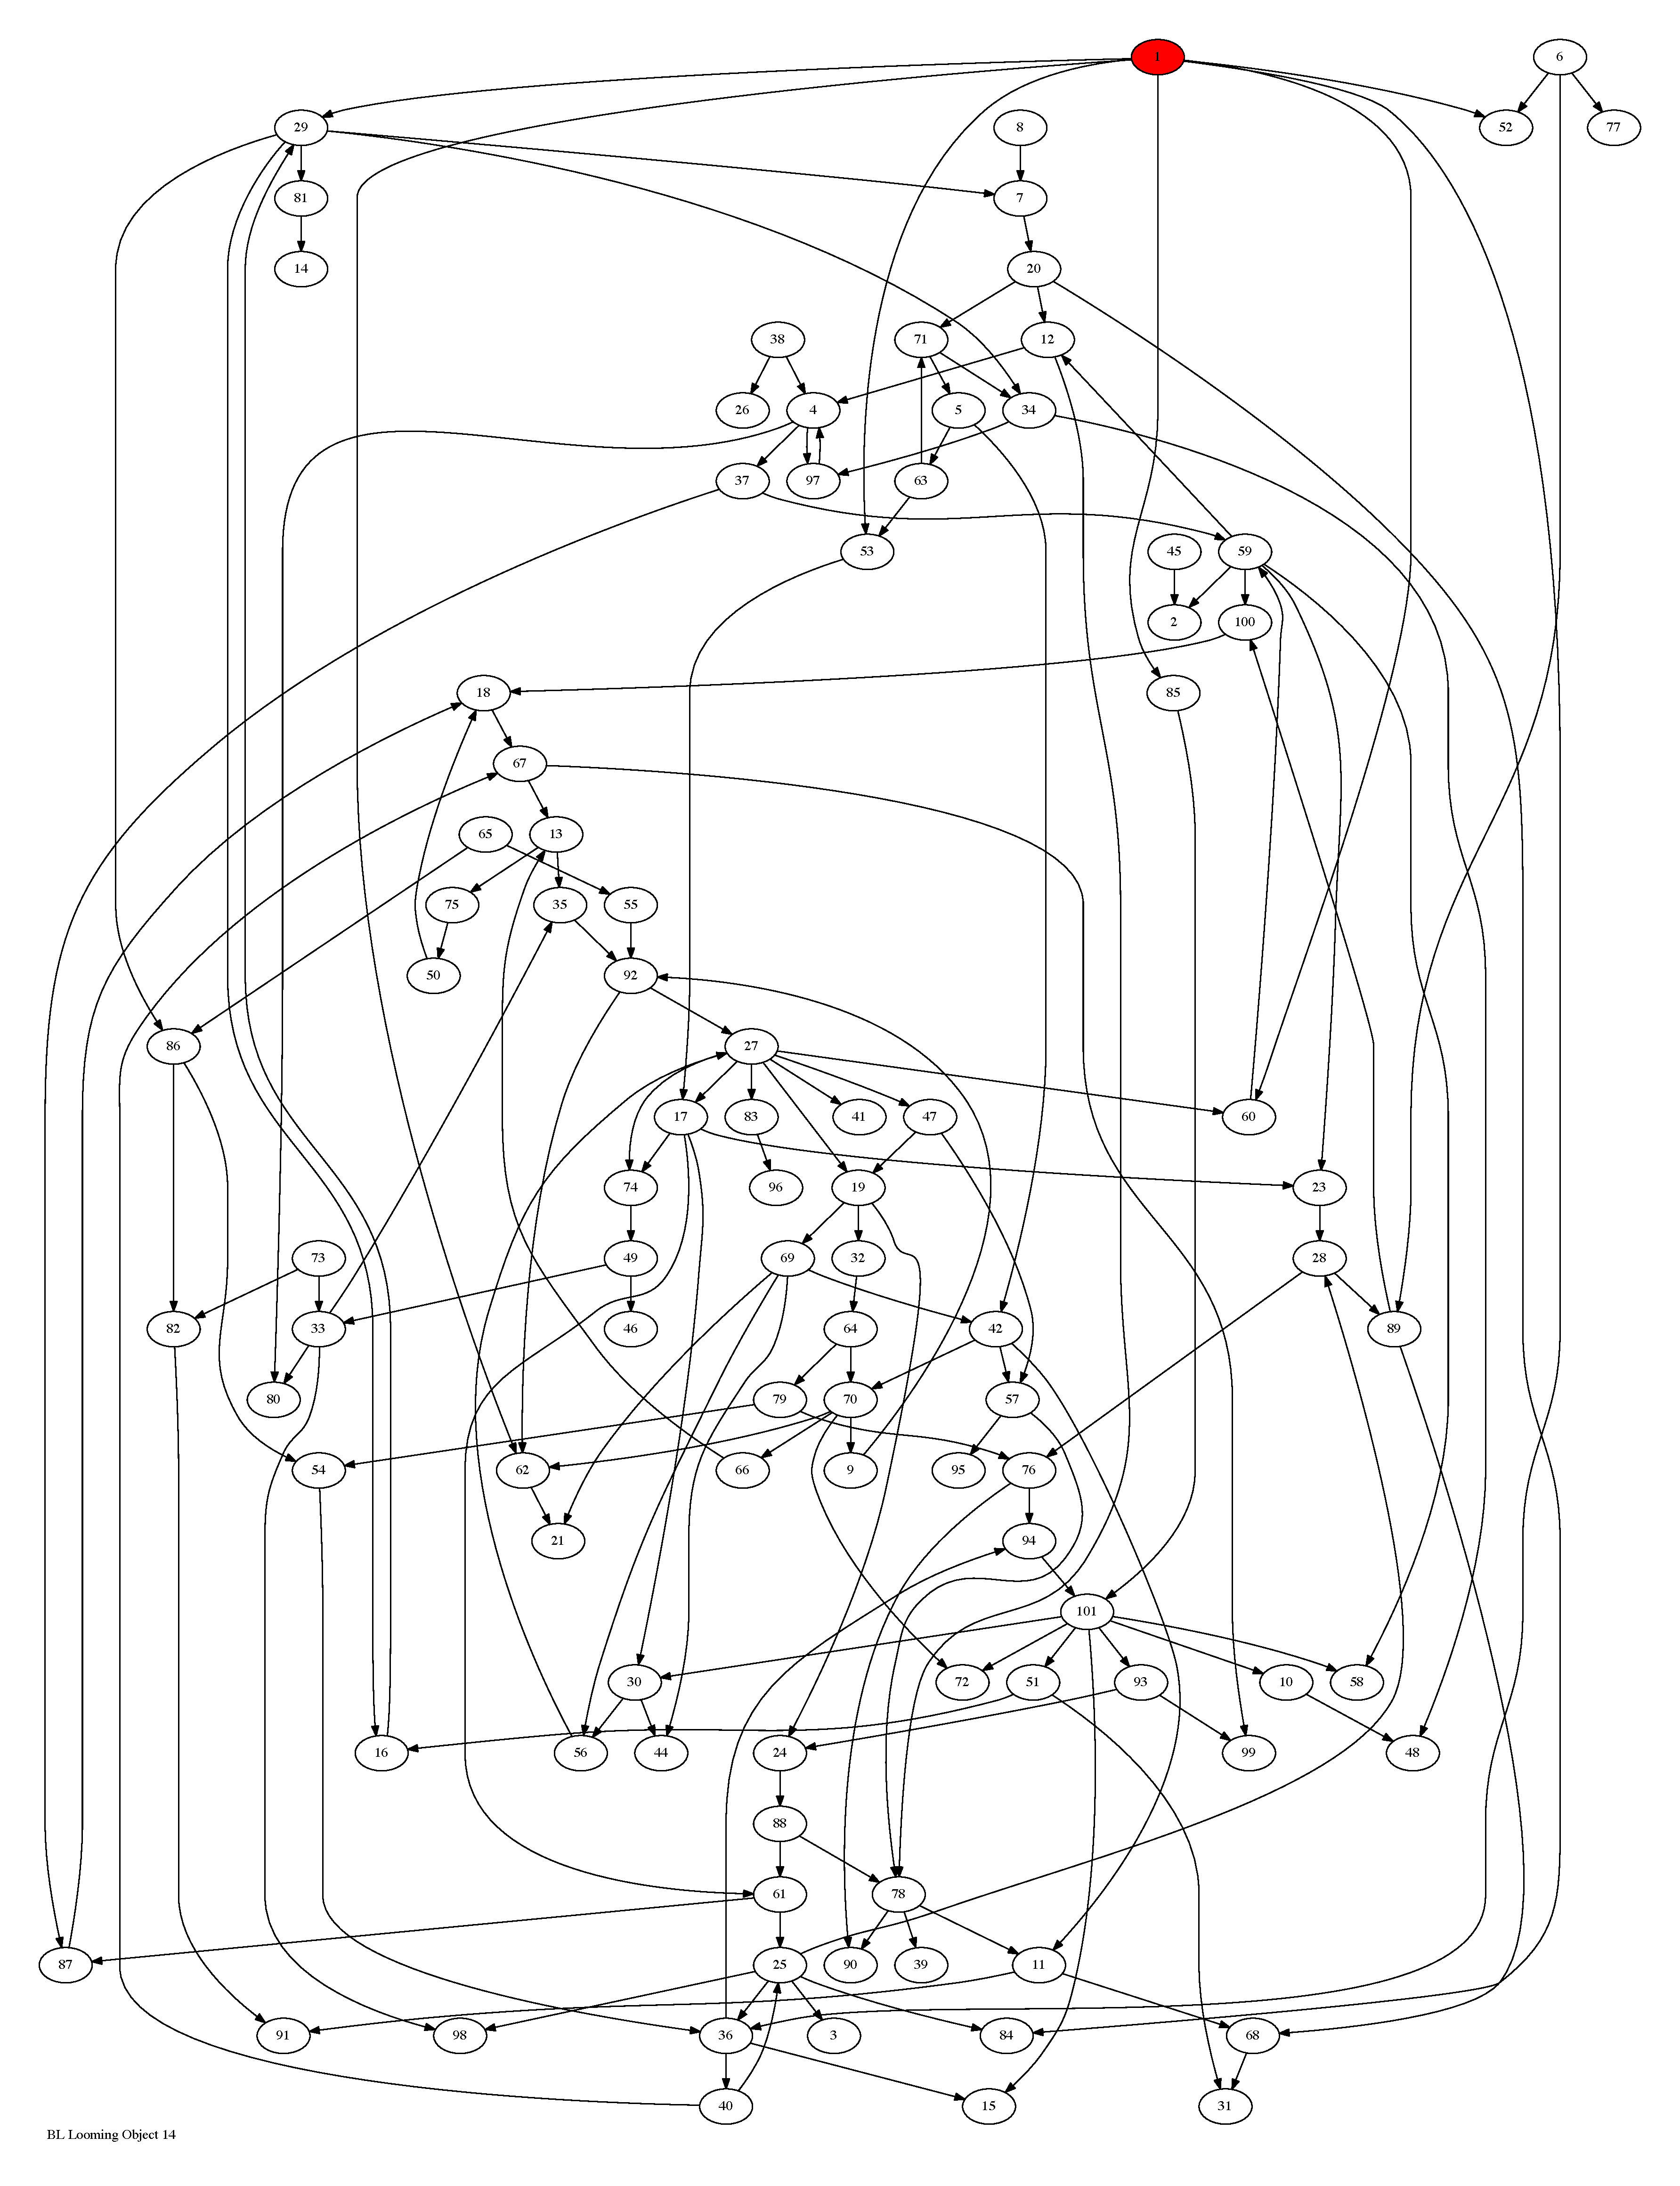
\includegraphics[max height=\textheight,max width=\textwidth]{bl_looming_objs/bl_loom_obj14_pp.pdf}

\newpage
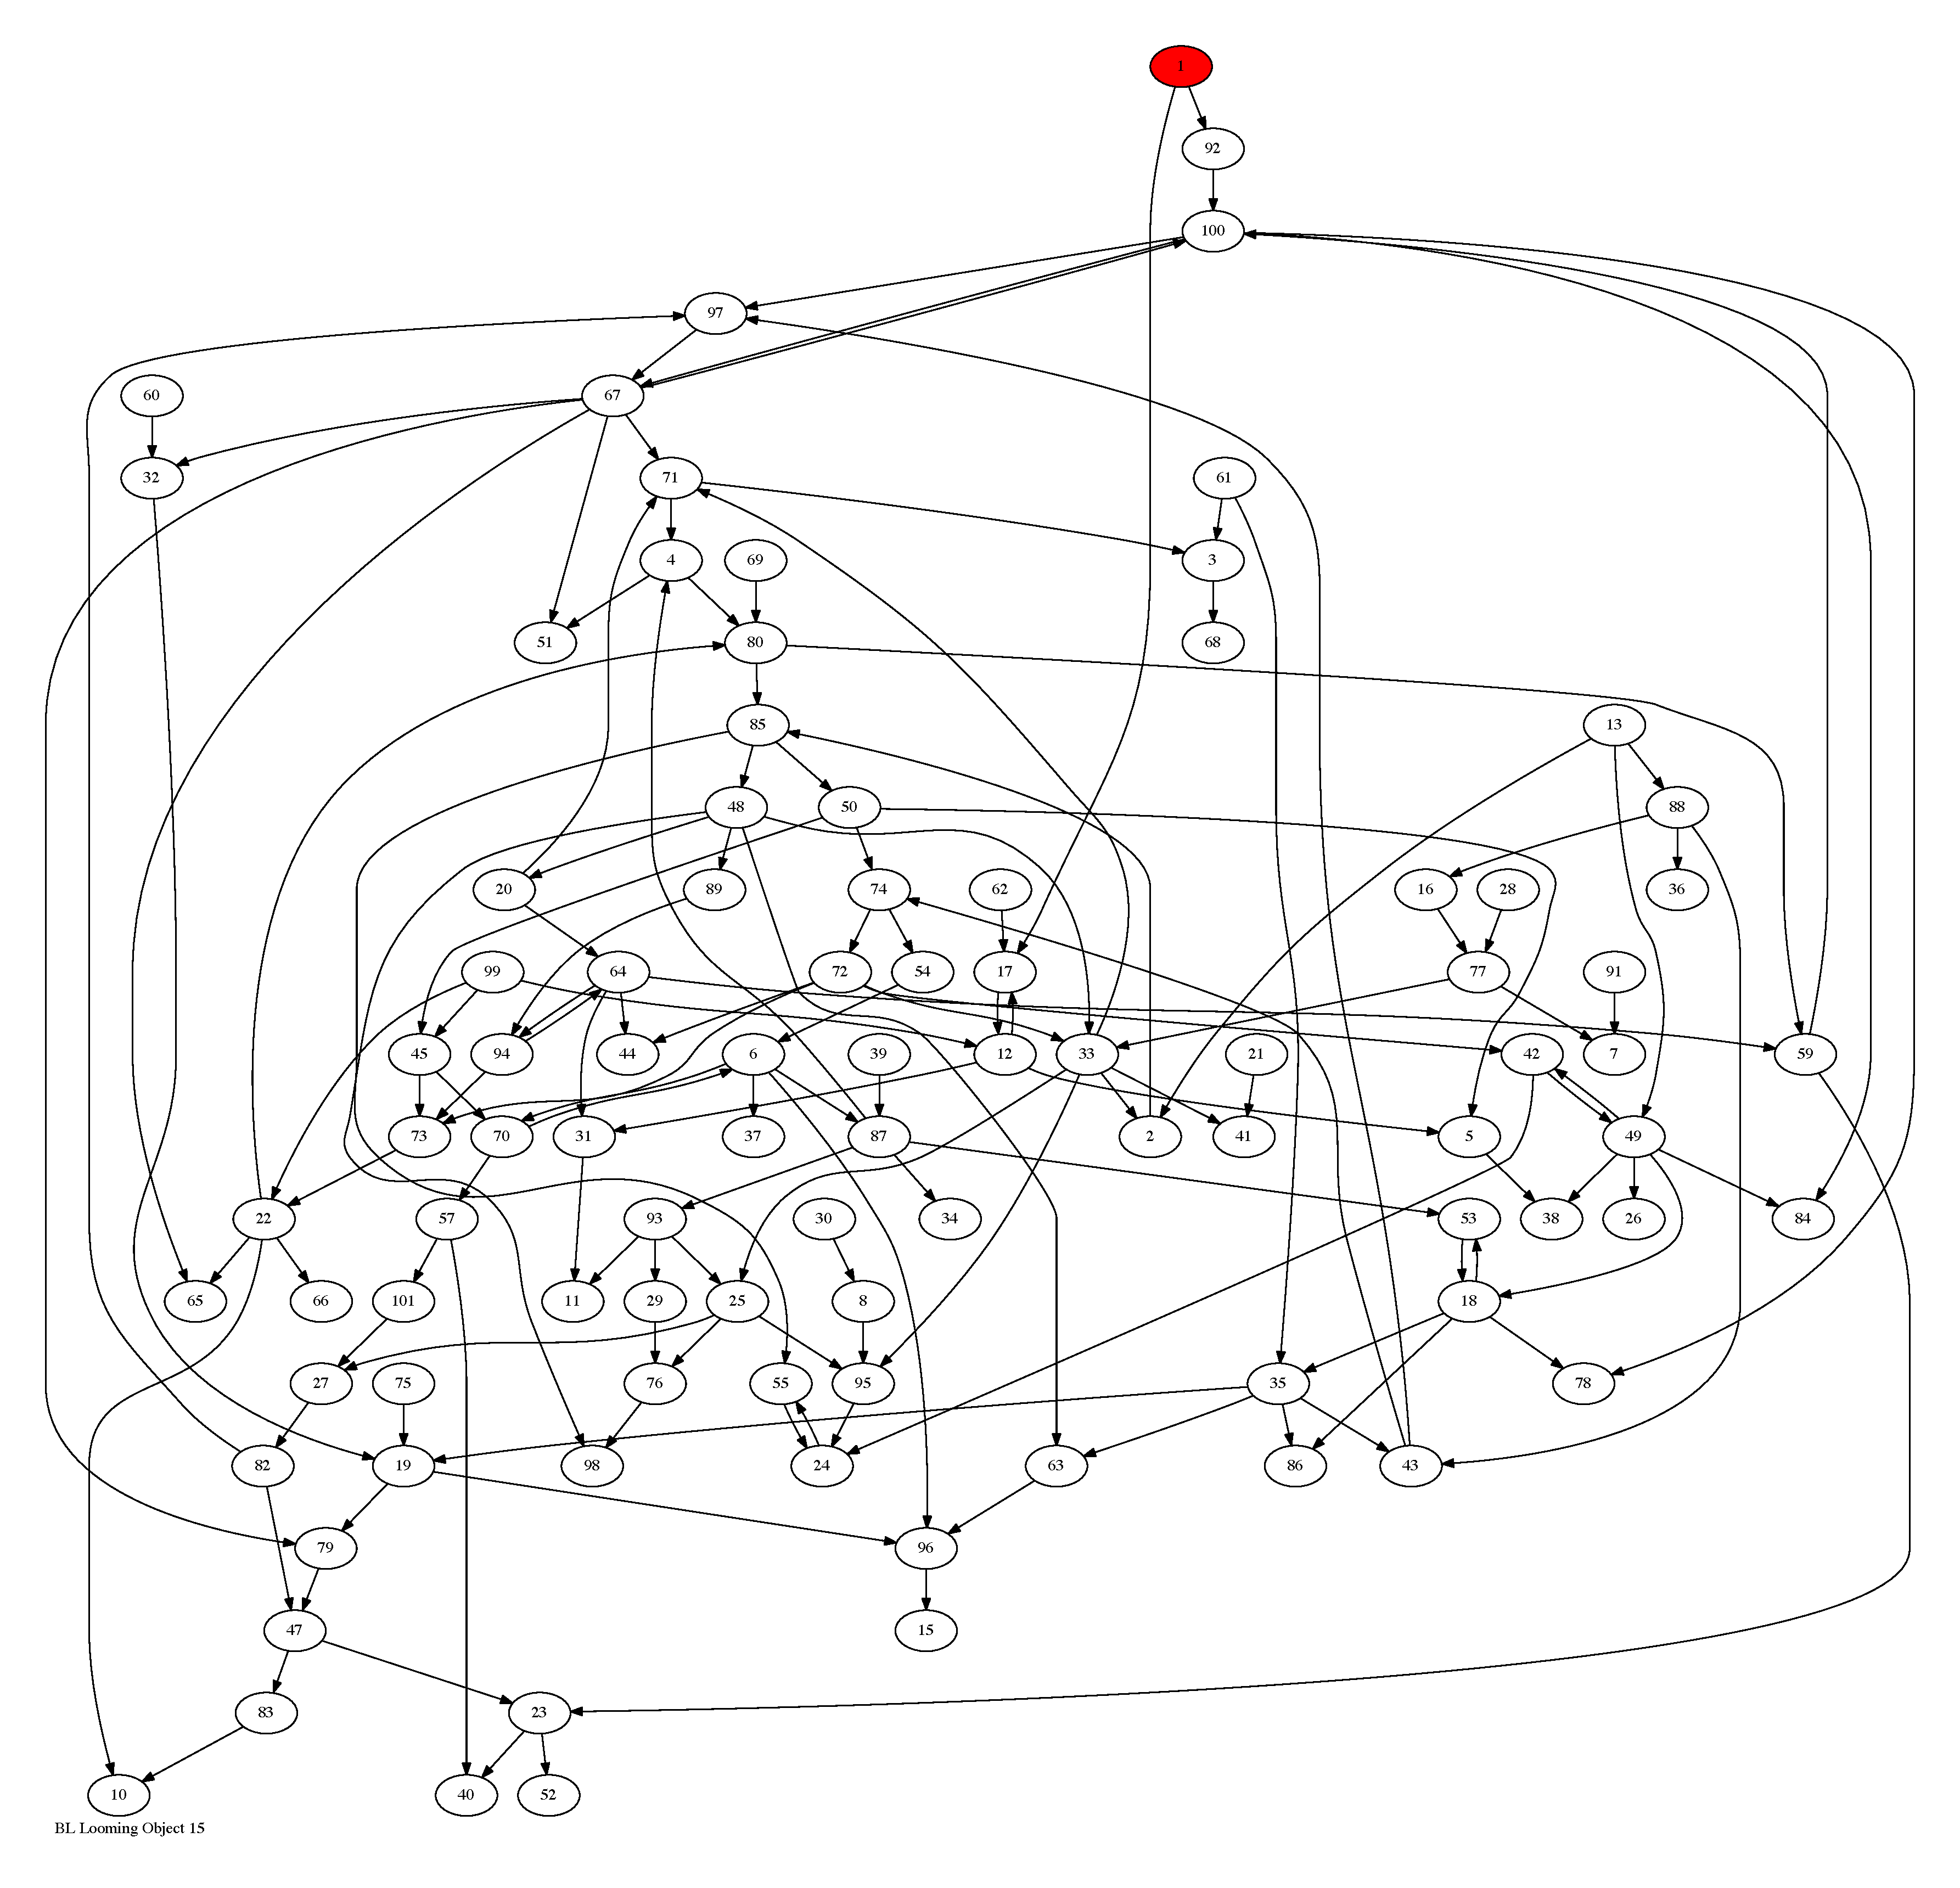
\includegraphics[max height=\textheight,max width=\textwidth]{bl_looming_objs/bl_loom_obj15_pp.pdf}

\newpage
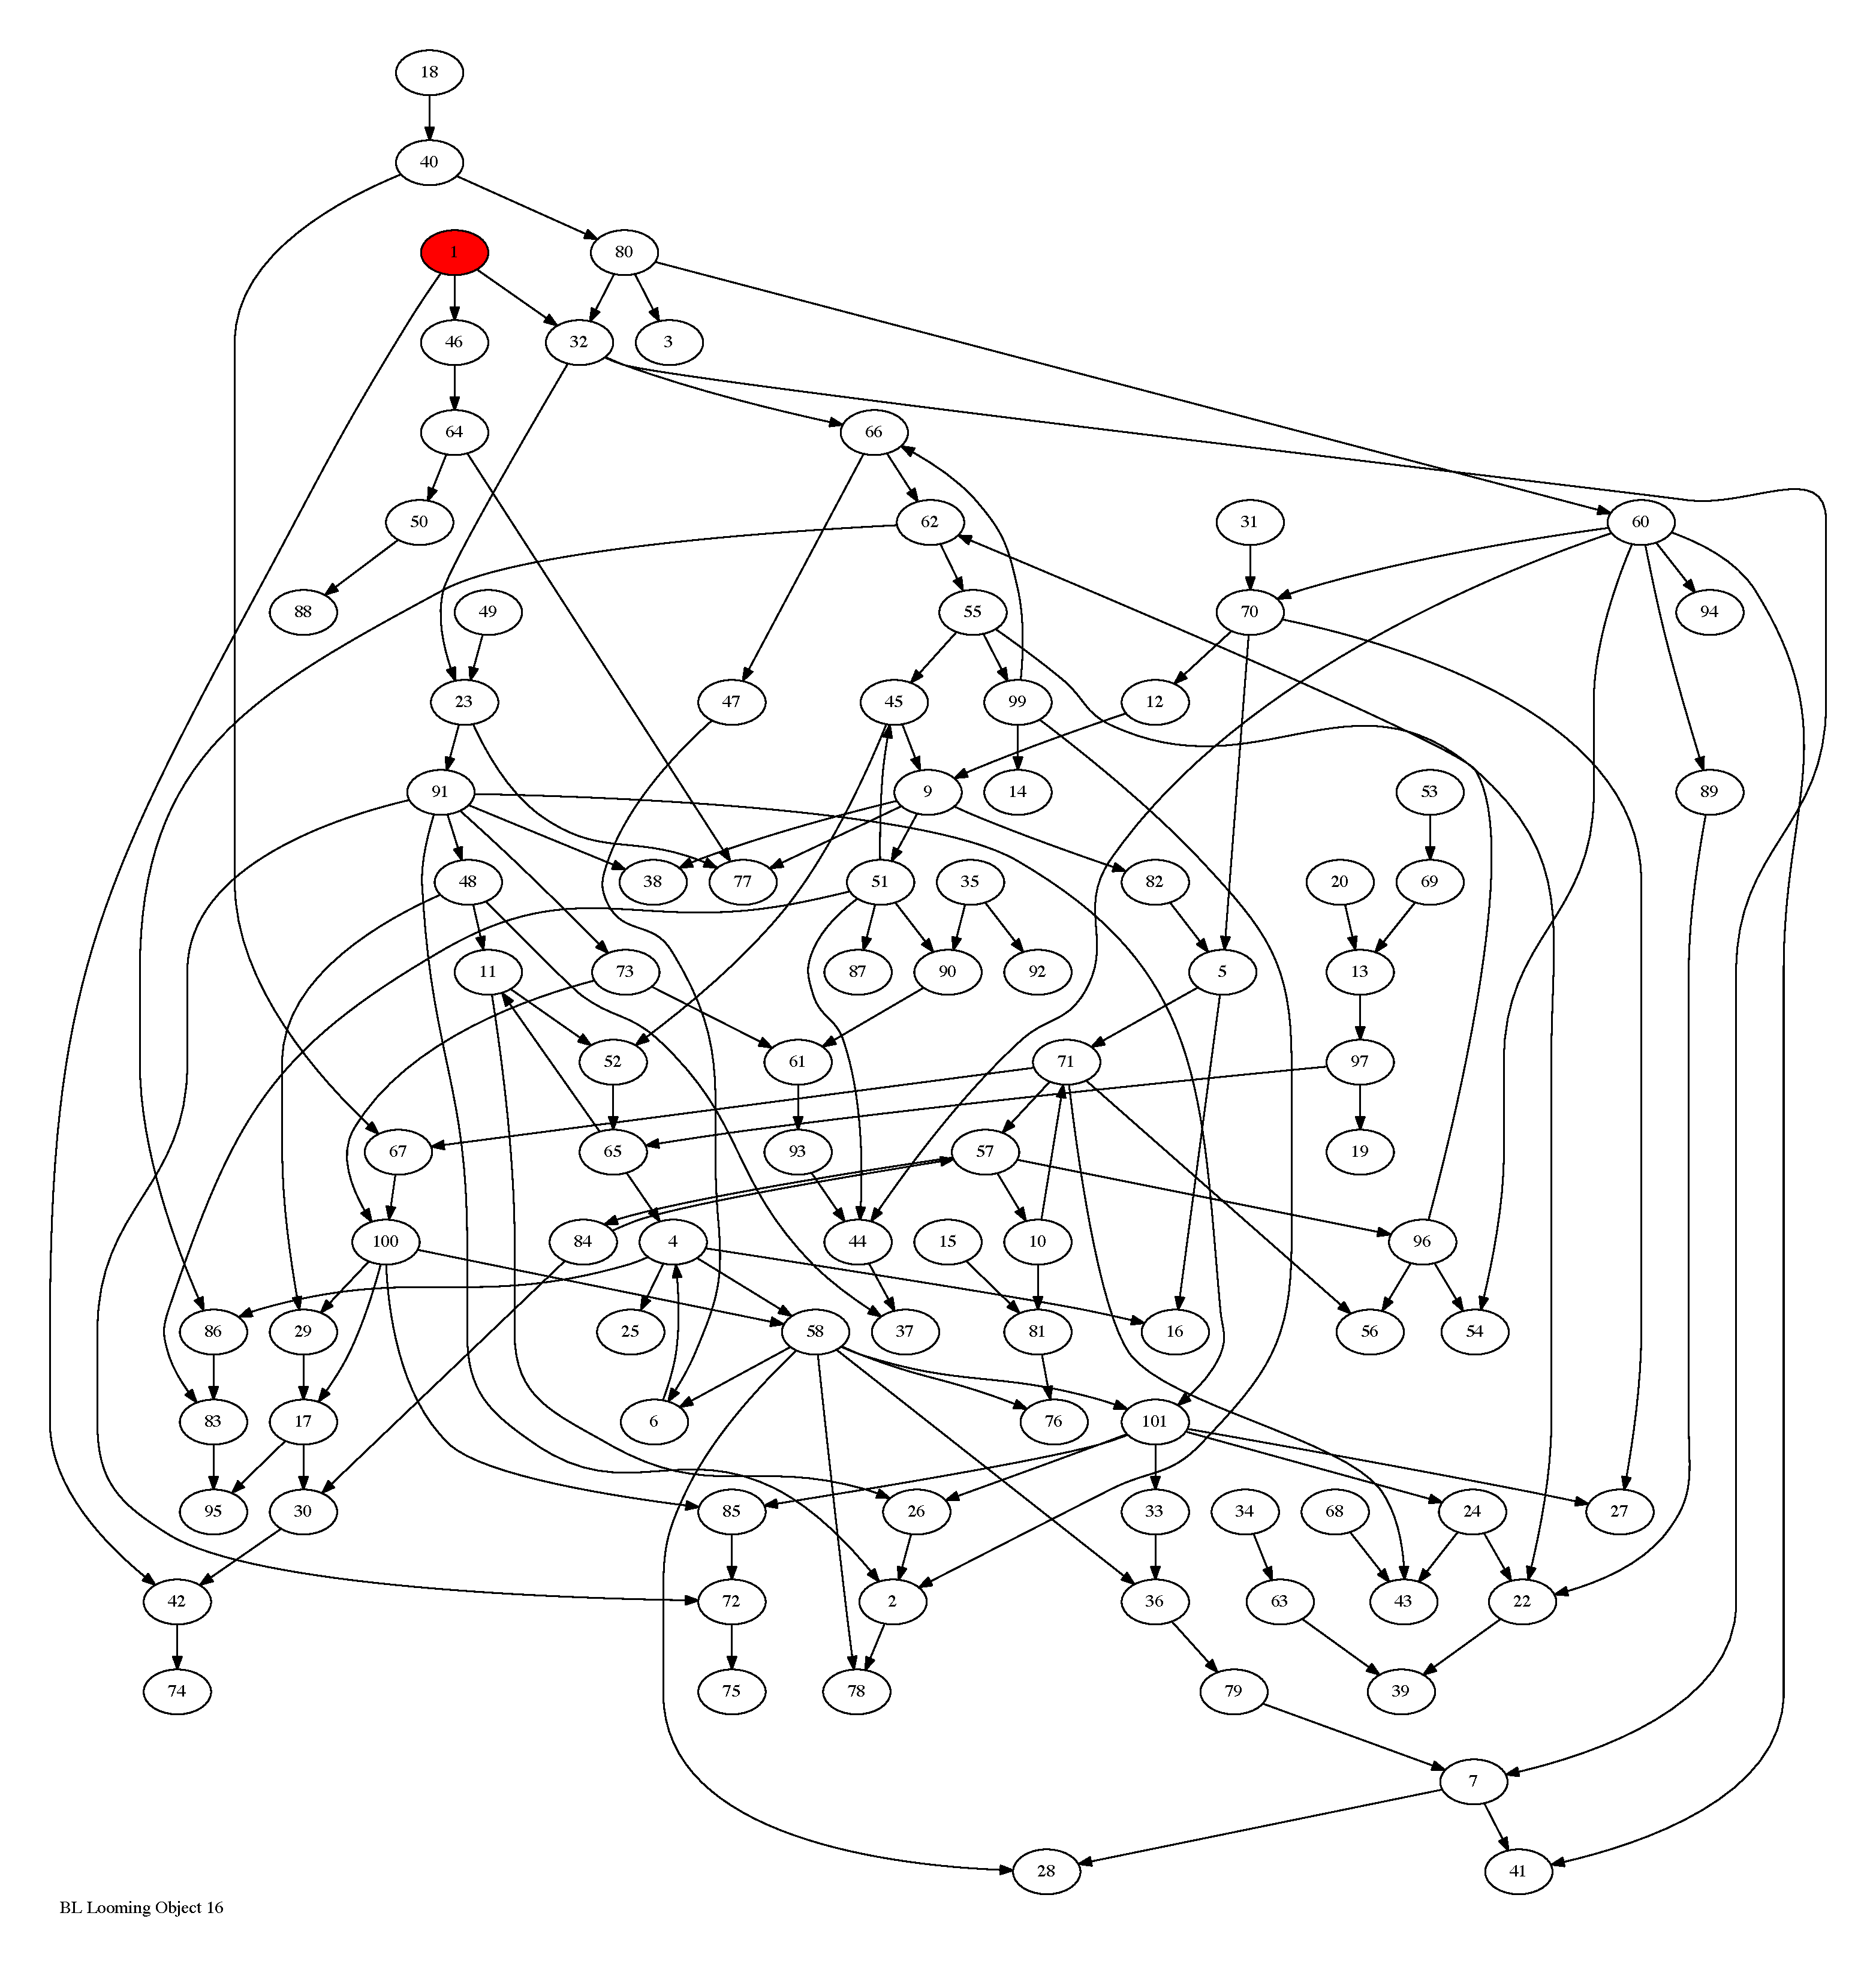
\includegraphics[max height=\textheight,max width=\textwidth]{bl_looming_objs/bl_loom_obj16_pp.pdf}

%%%%%%%%%%%%%%%%%%%%%%%%%%%%% LOOMING OBJECTS %%%%%%%%%%%%%%%%%%%%%%%%%%%%%%%%%

\newpage
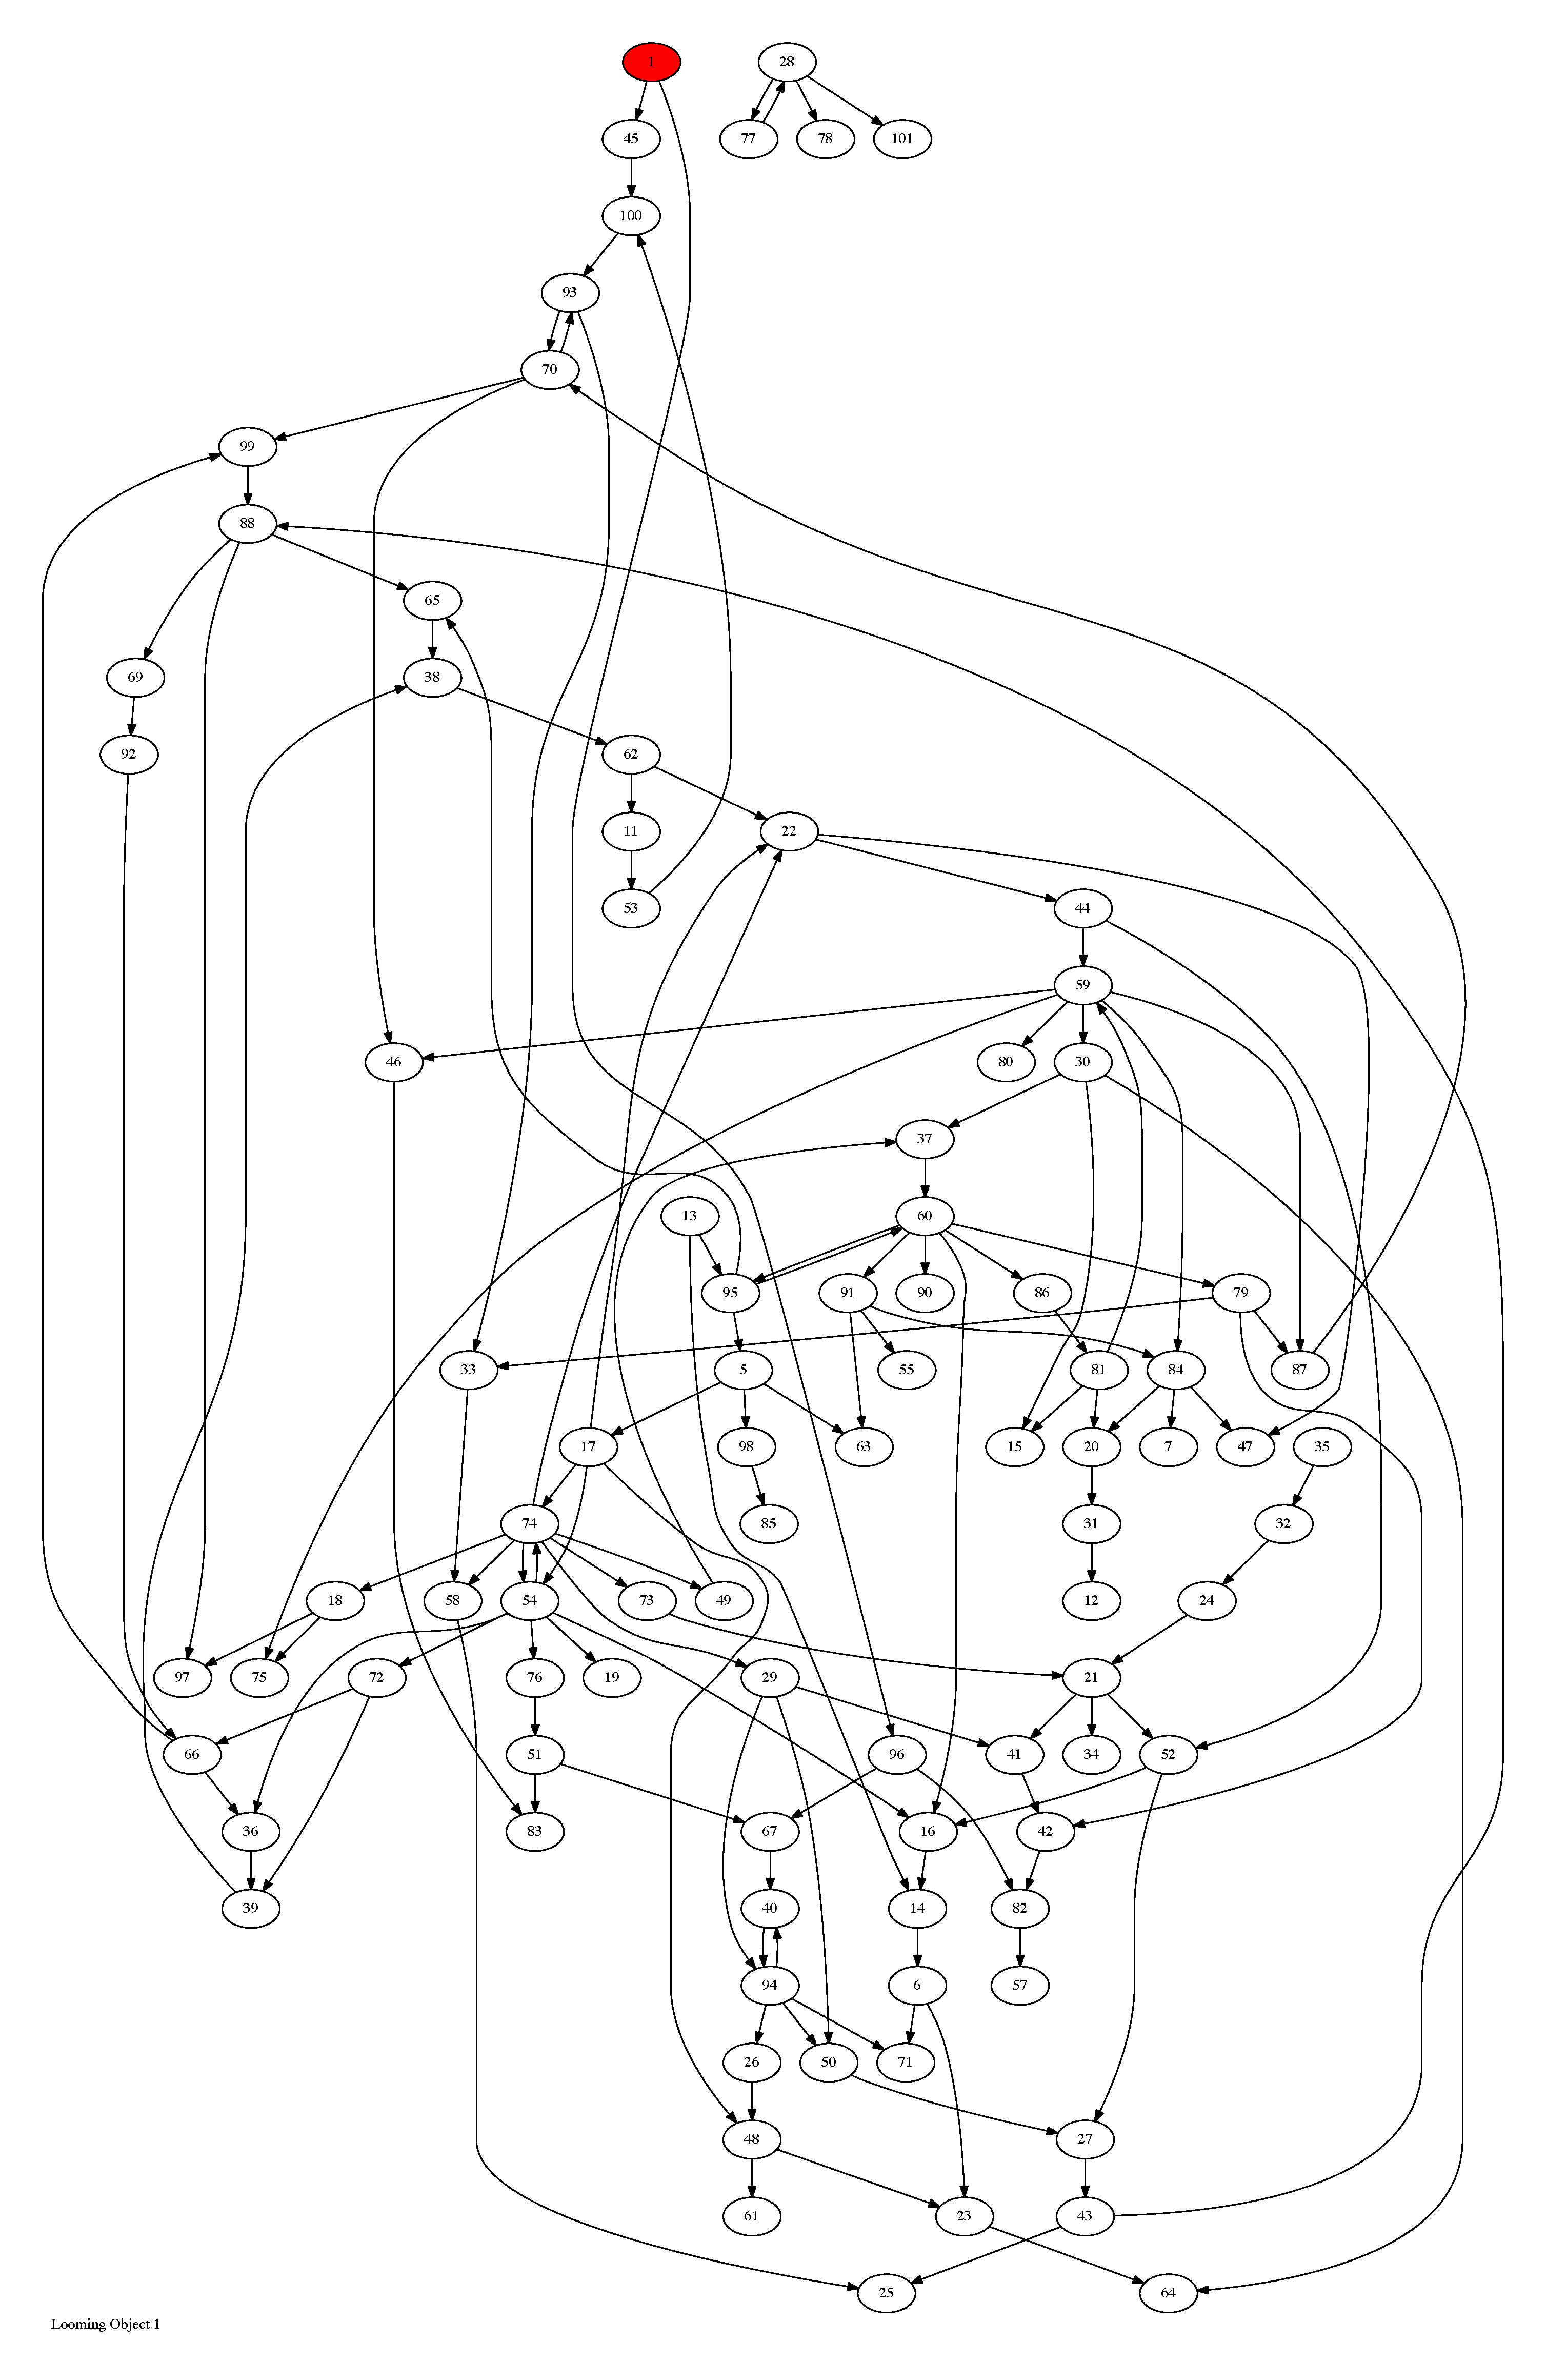
\includegraphics[max height=\textheight,max width=\textwidth]{looming_object/loom_obj1_pp.pdf}

\newpage
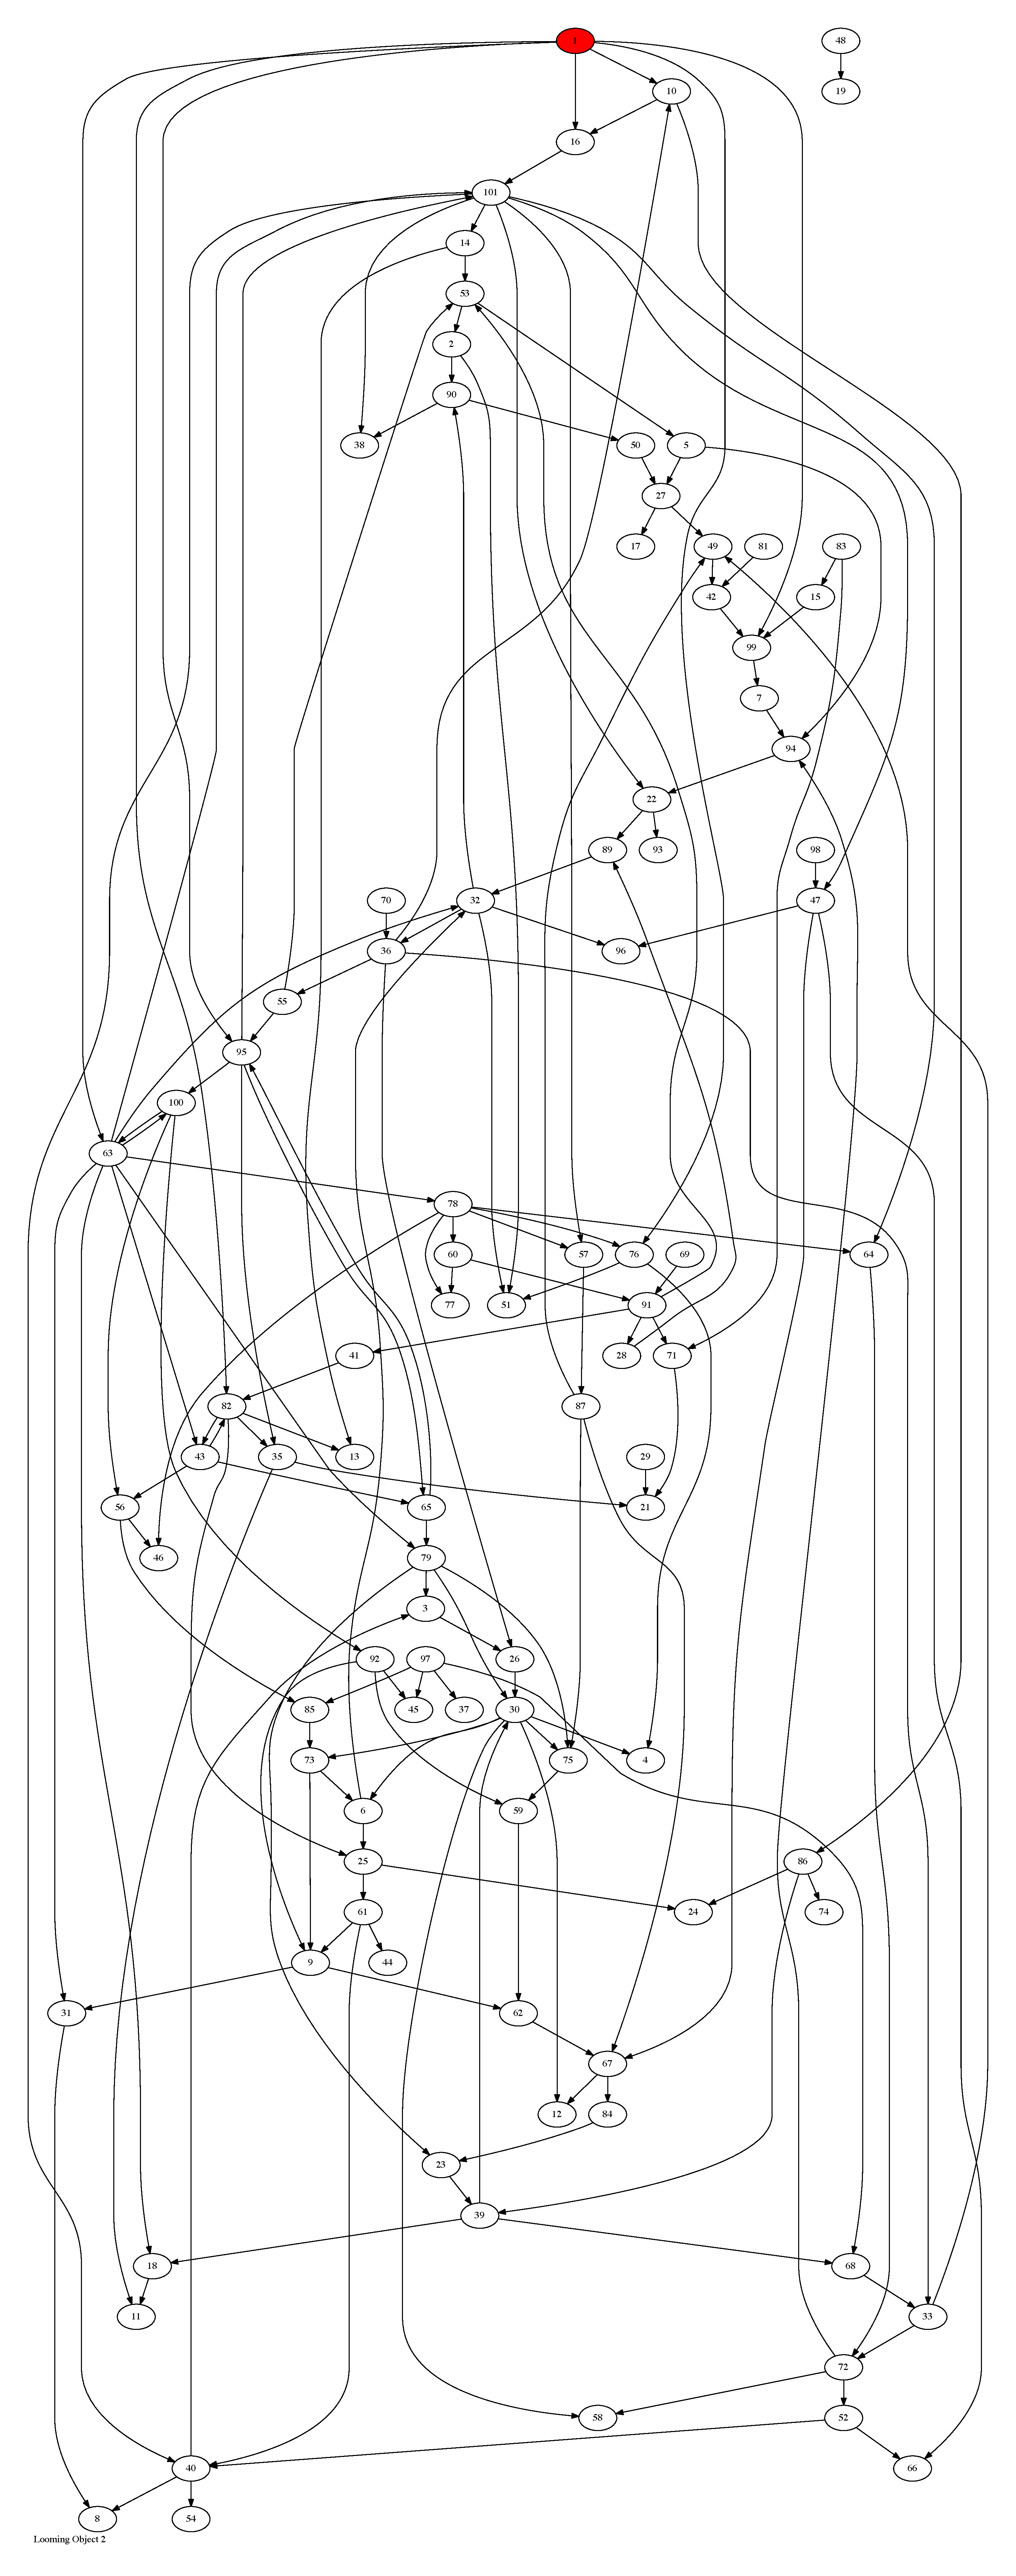
\includegraphics[max height=\textheight,max width=\textwidth]{looming_object/loom_obj2_pp.pdf}

\newpage
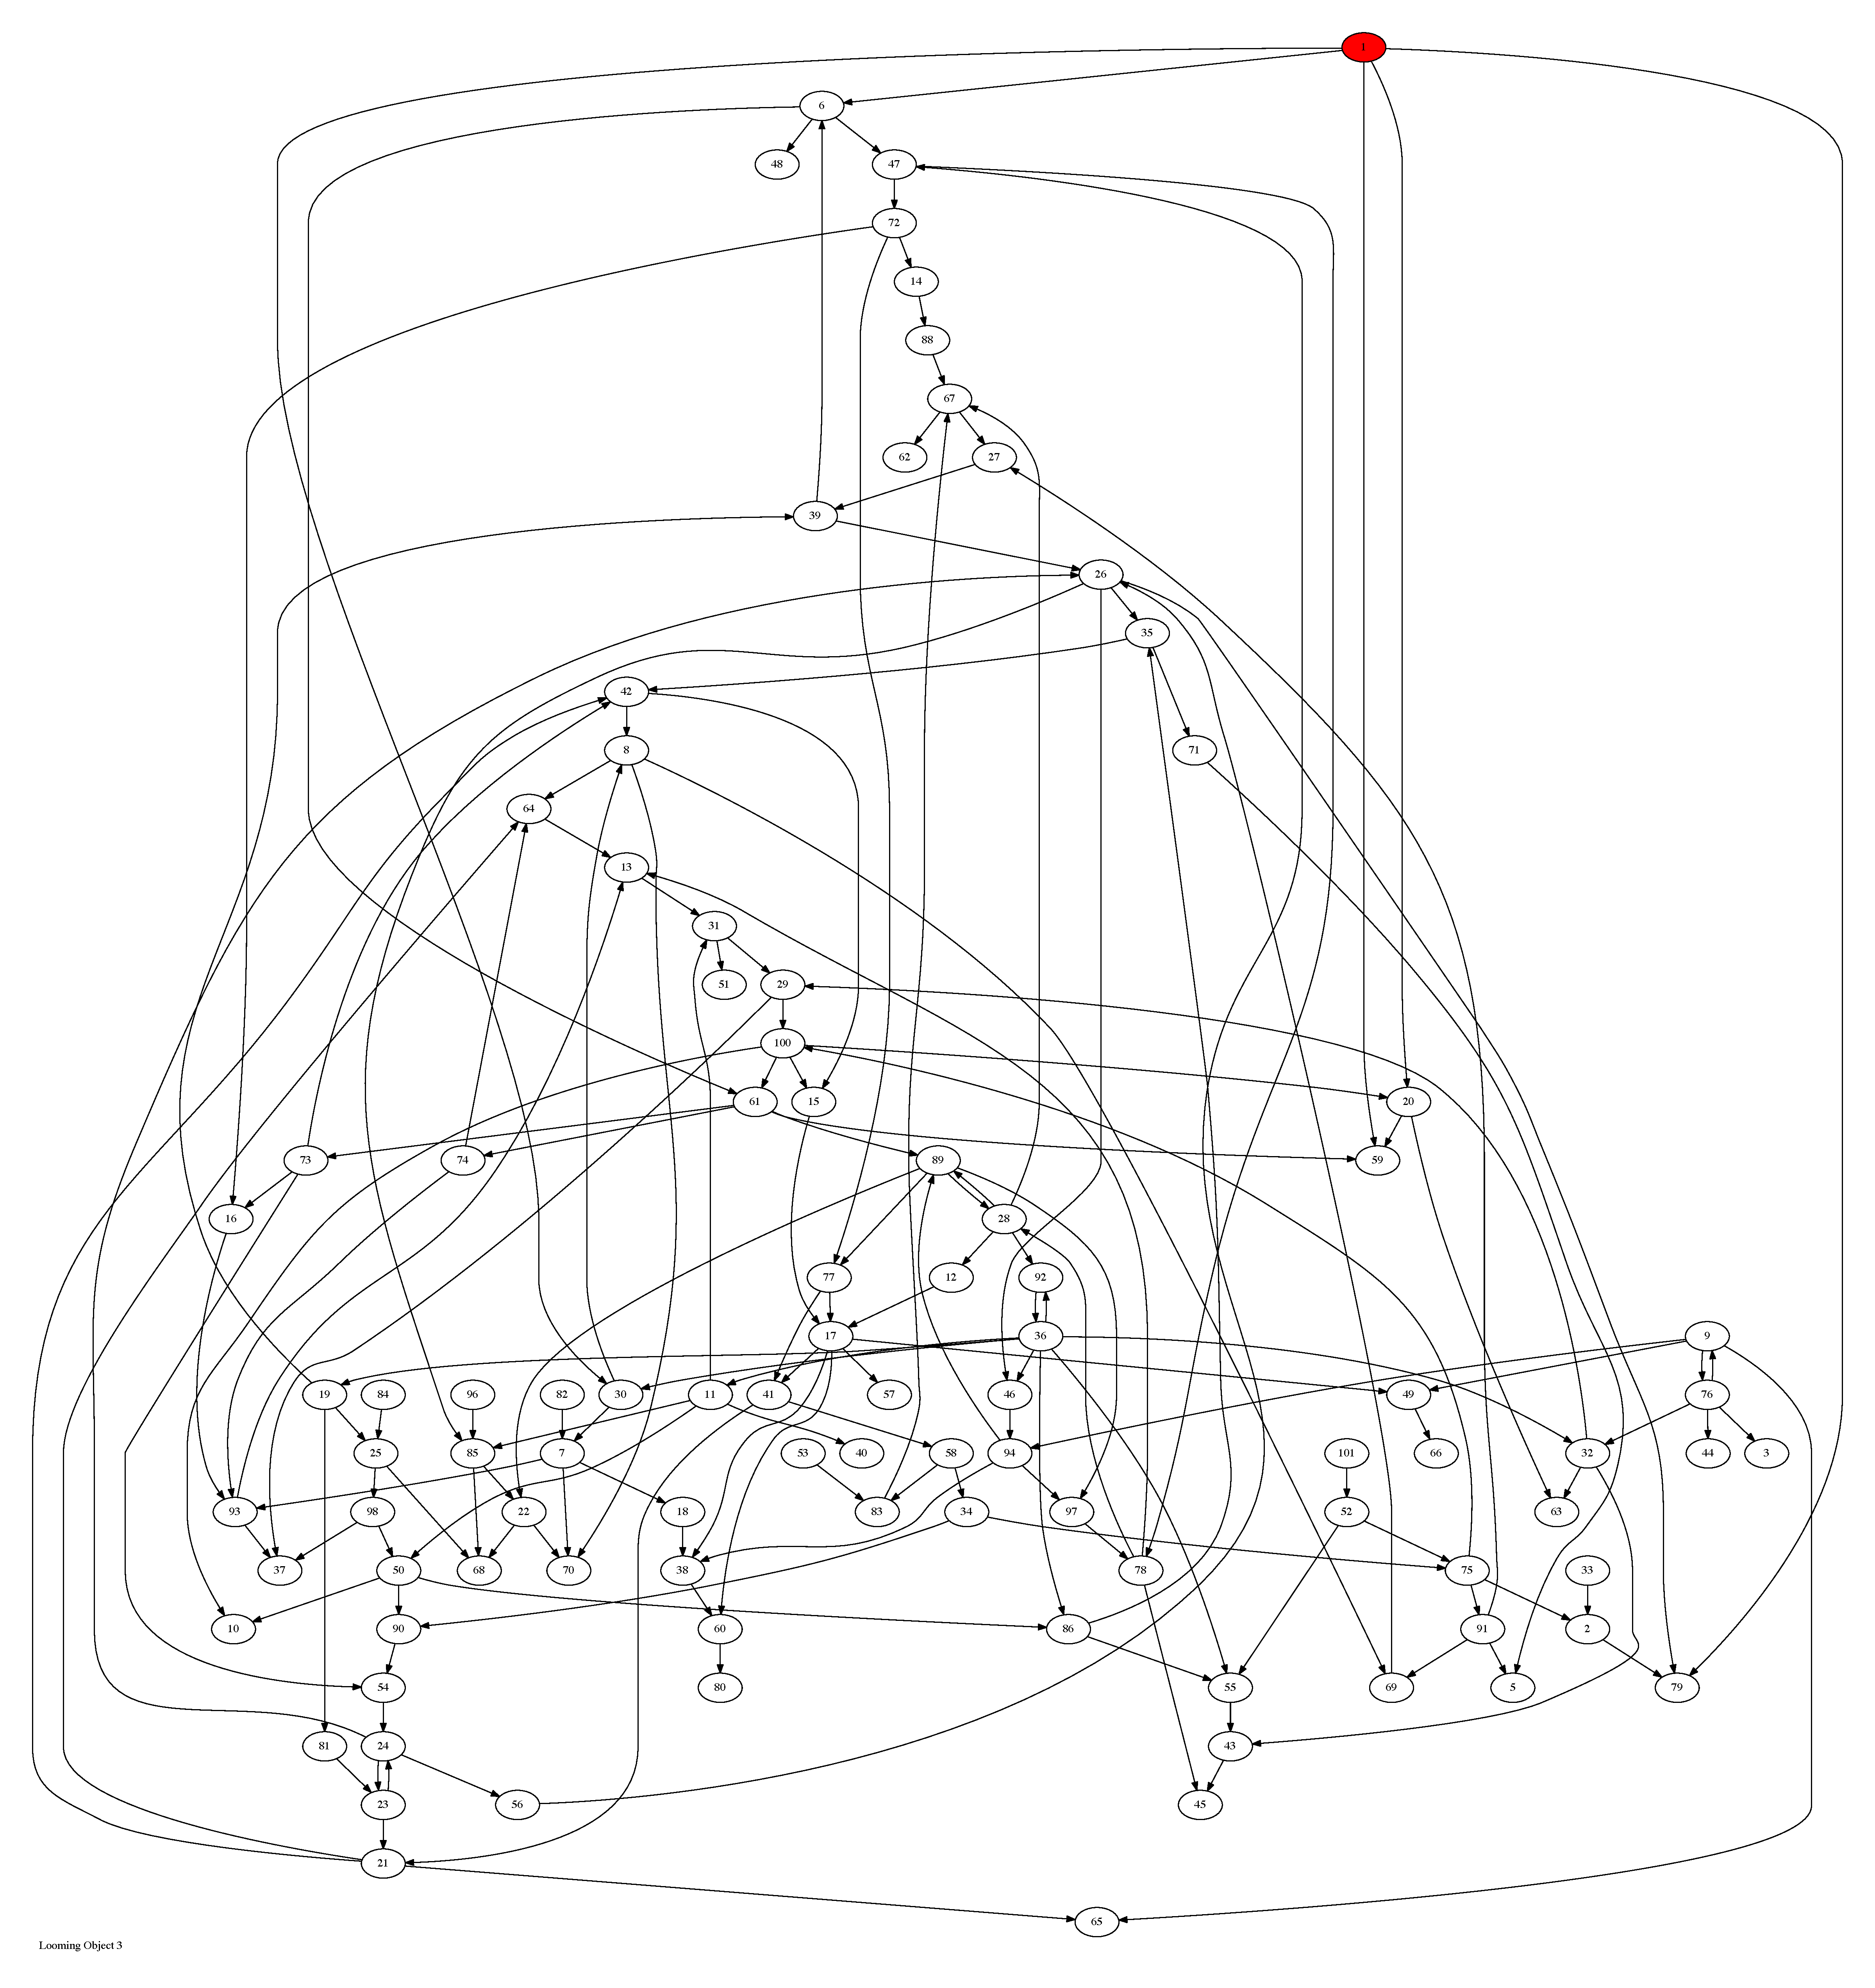
\includegraphics[max height=\textheight,max width=\textwidth]{looming_object/loom_obj3_pp.pdf}

\newpage
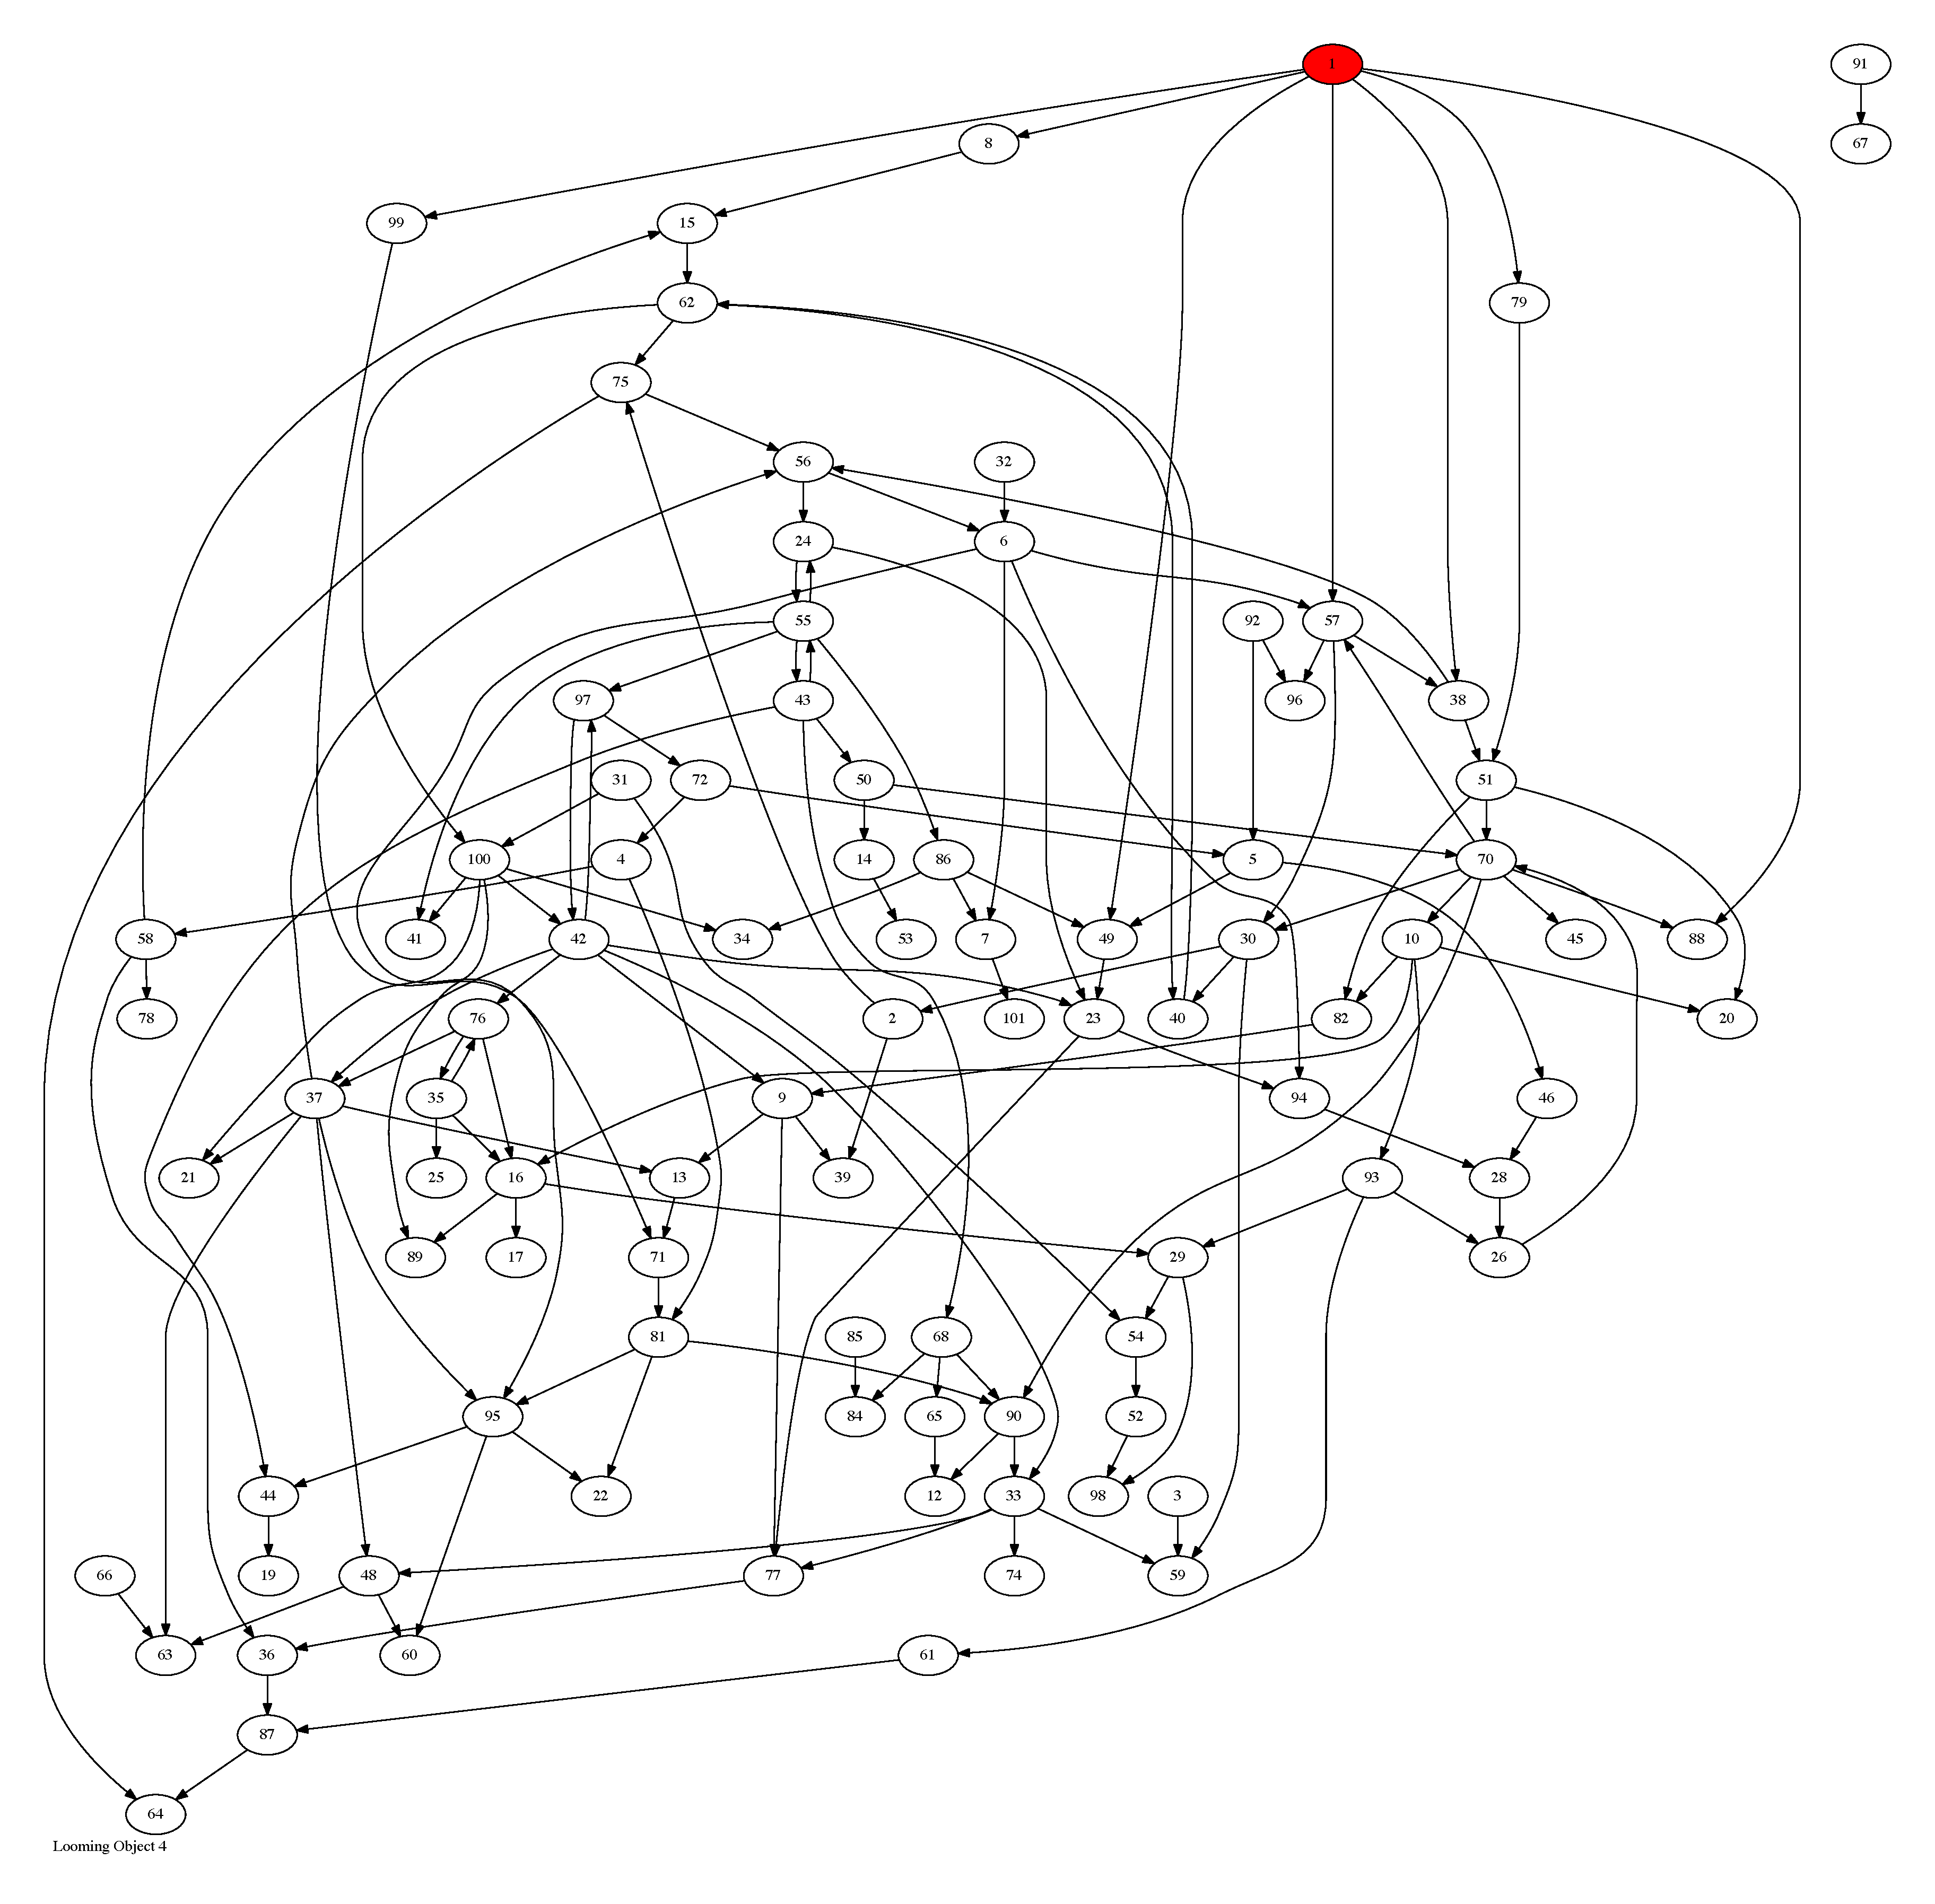
\includegraphics[max height=\textheight,max width=\textwidth]{looming_object/loom_obj4_pp.pdf}

\newpage
\includegraphics[max height=\textheight,max width=\textwidth]{looming_object/loom_obj5_pp.pdf}

\newpage
\includegraphics[max height=\textheight,max width=\textwidth]{looming_object/loom_obj6_pp.pdf}

\newpage
\includegraphics[max height=\textheight,max width=\textwidth]{looming_object/loom_obj7_pp.pdf}

\newpage
\includegraphics[max height=\textheight,max width=\textwidth]{looming_object/loom_obj8_pp.pdf}

\newpage
\includegraphics[max height=\textheight,max width=\textwidth]{looming_object/loom_obj9_pp.pdf}

\newpage
\includegraphics[max height=\textheight,max width=\textwidth]{looming_object/loom_obj10_pp.pdf}

\newpage
\includegraphics[max height=\textheight,max width=\textwidth]{looming_object/loom_obj11_pp.pdf}

\newpage
\includegraphics[max height=\textheight,max width=\textwidth]{looming_object/loom_obj12_pp.pdf}

\newpage
\includegraphics[max height=\textheight,max width=\textwidth]{looming_object/loom_obj13_pp.pdf}

\newpage
\includegraphics[max height=\textheight,max width=\textwidth]{looming_object/loom_obj14_pp.pdf}

\newpage
\includegraphics[max height=\textheight,max width=\textwidth]{looming_object/loom_obj15_pp.pdf}

\newpage
\includegraphics[max height=\textheight,max width=\textwidth]{looming_object/loom_obj16_pp.pdf}

\end{document}
